\documentclass[twoside,a4paper,11pt]{article}
\usepackage{wrapfig}
\usepackage{graphicx}
\usepackage{graphics}
\usepackage{amsmath}
\usepackage{amsfonts}
\usepackage[T1]{fontenc}
\usepackage{amssymb}
\usepackage[font=footnotesize, singlelinecheck=false, labelfont=bf]{caption}
\usepackage{array}
\usepackage{multirow}
\usepackage{setspace}
\usepackage{hyperref}
\usepackage{verbatim}
\usepackage{epstopdf}
\usepackage{textcomp}
\usepackage{nicefrac}
\usepackage{xspace}
\usepackage{lineno}
\usepackage[footnotesize, bf, hang, raggedright]{subfigure}
\usepackage{charter}
\usepackage[expert]{mathdesign}
\usepackage[bottom]{footmisc}
\usepackage[english]{babel}
\usepackage{tikz}
\usepackage{multirow}
\usetikzlibrary{arrows}

\onehalfspacing
\usepackage[left=2.9cm,right=2.9cm,top=3cm,bottom=4.5cm]{geometry}

\newcommand{\subfigureautorefname}{\figurename}
\newcommand\geant{\textsc{Geant\,4}\xspace}
\newcommand\mokka{\textsc{Mokka}\xspace}
\newcommand\ddhep{\textsc{DD4hep}\xspace}

\usepackage{xcolor}
\usepackage[printwatermark]{xwatermark}
\newwatermark[allpages,color=gray!30,angle=45,scale=3,xpos=-10,ypos=0]{Draft}

\usepackage{titlesec} 
\titleformat{\section}[hang]{
\usefont{T1}{qhv}{b}{n}\selectfont} % "qhv" - TeX Gyre Heros, "b" - bold
{} 
{0em}
{\hspace{-0.4pt}\Large \thesection\hspace{0.6em}}

\usepackage[subfigure]{tocloft} % subfigure option only if using subfigure package
\renewcommand{\cfttoctitlefont} % ToC title
             {\usefont{T1}{qhv}{b}{n}\selectfont\huge}
\renewcommand{\cftsecfont} % section titles
             {\usefont{T1}{bch}{b}{n}\selectfont}
\renewcommand{\cftsubsecfont} % subsection titles
             {\usefont{T1}{bch}{m}{n}\selectfont} 
\renewcommand{\cftsecpagefont} % section page numbers
             {\cftsecfont} 
\renewcommand{\cftsubsecpagefont} % subsection page numbers
             {\cftsubsecfont}

\newcommand\MyLBrace[2]{%
  \left.\rule{0pt}{#1}\right\}\text{#2}}

\linenumbers
\setcounter{tocdepth}{2}

\begin{document}
\selectlanguage{english}
\begin{titlepage}
\begin{flushright}
CALICE Analysis Note CAN-057\\
v1.0\\
October 7, 2016 \\
\end{flushright}

\begin{center}
\vspace*{\fill}
\begin{LARGE} \textbf{Timing Resolution in Testbeam of the CALICE Analog Hadronic Calorimeter} \end{LARGE} \\ [10ex]
\begin{Large} The CALICE Collaboration \footnote{Corresponding authors: \\ Eldwan Brianne; eldwan.brianne@desy.de; Katja Krueger; katja.krueger@desy.de}\\ [10ex]
\end{Large}

\begin{large}
\textbf{Abstract} \\
\end{large}
\end{center}
This note presents results obtained with the CALICE engineering prototype consisting of the \emph{Analog Hadronic Calorimeter} at the CERN testbeam campaign in 2015. The analysis includes timing distributions for muon, electron and pion beams. The results are compared to several \geant version 10.1 physics lists.\\
\\

\textit{
This note contains preliminary CALICE results, and is for the use of members of the CALICE Collaboration and others to whom permission has been given.}

\end{titlepage}

\clearpage
\tableofcontents
\newpage
\section{Introduction}

The International Large Detector (ILD) \cite{ILC_TDR} considers a highly granular hadronic calorimeter using iron absorbers to achieve a compact detector with the best jet energy resolution around 3-4\% at 250 GeV satisfying the space constrain imposed by the solenoid magnet. Timing measurements in a calorimeter can be used to reject pile-up events like at the LHC or CLIC due to the bunch-to-bunch spacing of 25 and 0.5 ns respectively. Also the high level of $\gamma\gamma \rightarrow$ hadrons could be rejected by using timing information of the calorimeter in order to limit the impact of the background on physics measurements. Novel techniques of using time information to improve energy reconstruction could be used \cite{IEEE_timing}.\\
In the hadronic calorimeter, the timing precision is highly influenced by the time structure of the shower itself. A hadronic shower possesses several timing components related to different processes happening in the shower. A fast component related to instantaneous highly energetic deposits from high-energy hadrons and electromagnetic sub-showers. A slow component due to neutron scattering, nuclear-recoil and photons from nuclear processes, this component can last up to several milliseconds. Apart from physics processes, the measured hit time is influenced by the active medium used as well as the electronics. Time constants in the active medium such as scintillation decay time can affect the measurement.\\
The performance of the ILD relies on simulation studies based on \geant, it is important to study how well the simulation performs to reproduce the time structure of hadronic showers observed in data. The CALICE Analog Hadronic Calorimeter (AHCAL) technological prototype has been installed in the SPS CERN facilities in July and August 2015 in order to provide measurements using plastic scintillators. The goal of this study is to improve our knowledge about hadronic showers especially about its time evolution and time correlation within the calorimeter. This note will describe the timing calibration procedure of the AHCAL first, the comparison with simulation for muons and electrons and finally a comparison with pion data.

\section{The CERN 2015 Testbeam Setup}

The datasets used in this note were collected during the testbeam campaign at CERN Super Proton Synchrotron (SPS) in July 2015. The SPS beamline provides secondary beams of hadrons, electrons and muons in a wide particle momenta range from 10 to 360 GeV/c. More details on the beamline are available in \cite{SPSBeamLine}.

\subsection{The CALICE AHCAL technological prototype}

In the July 2015 testbeam period, the CALICE AHCAL technological prototype setup consisted of 38 steel absorber plates, 19 mm thick corresponding to a depth of approximately 40 $X_0$ ($\sim$ 4.5 nuclear interaction length $\lambda_{n}$). The active layers consisted of a iron cassette, 1 mm thick, a HCAL Base Unit (HBU) of an area of $36\times36$ cm$^2$, hosting the integrated readout electronics and a $30\times30\times3$ mm$^3$ plastic scintillator tile wrapped in a reflective foil. Each plastic tile is read out individually by a SiPM. The layers consisted of either 1 or 4 HBUs as illustrated in figure \ref{fig:detector_layout}. 

\begin{figure}[htbp]
	\subfigure[%Picture of the AHCAL steel stack during the CERN testbeam.
	\label{fig:stack_steel}] {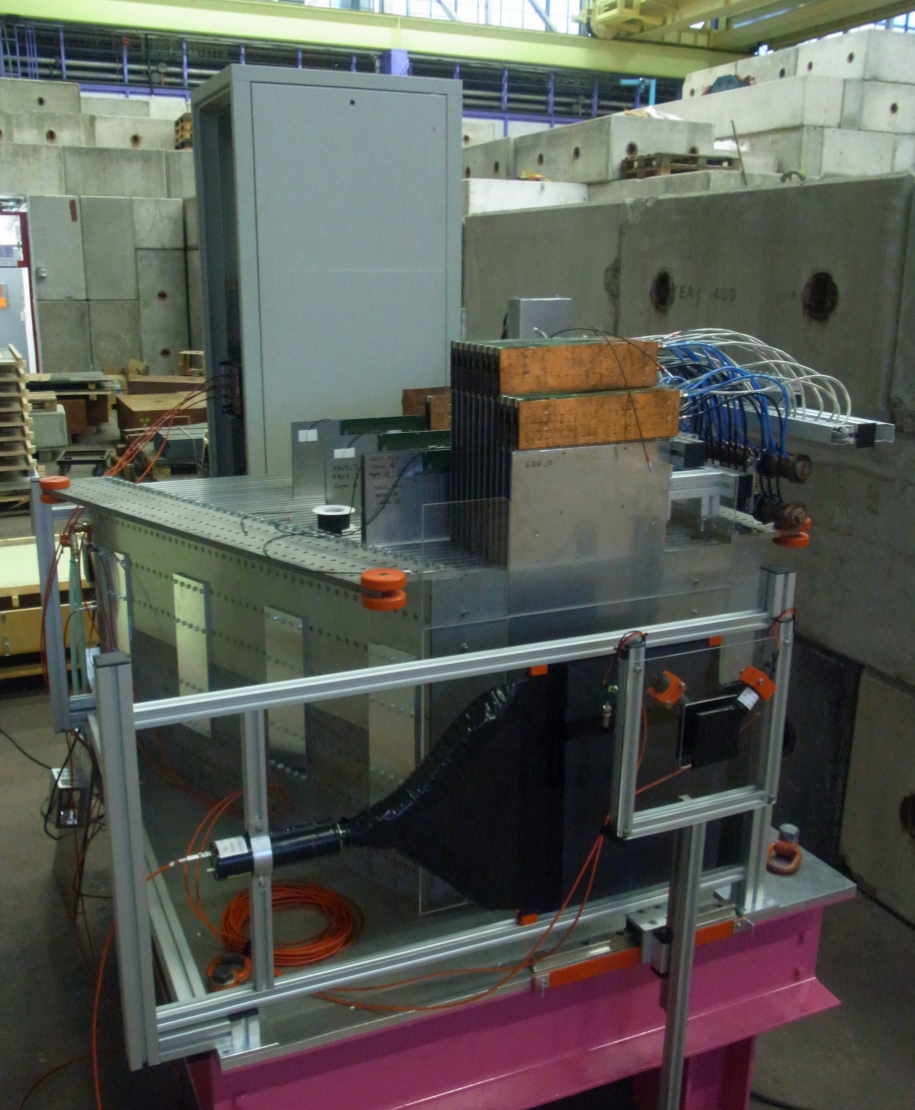
\includegraphics[width=0.35\textwidth]{fig/steel_stack_ps.png}}\hfill
	\subfigure[%Detector layout of the CALICE AHCAL during the 2015 July Testbeam at the SPS.
	\label{fig:detector_layout}] {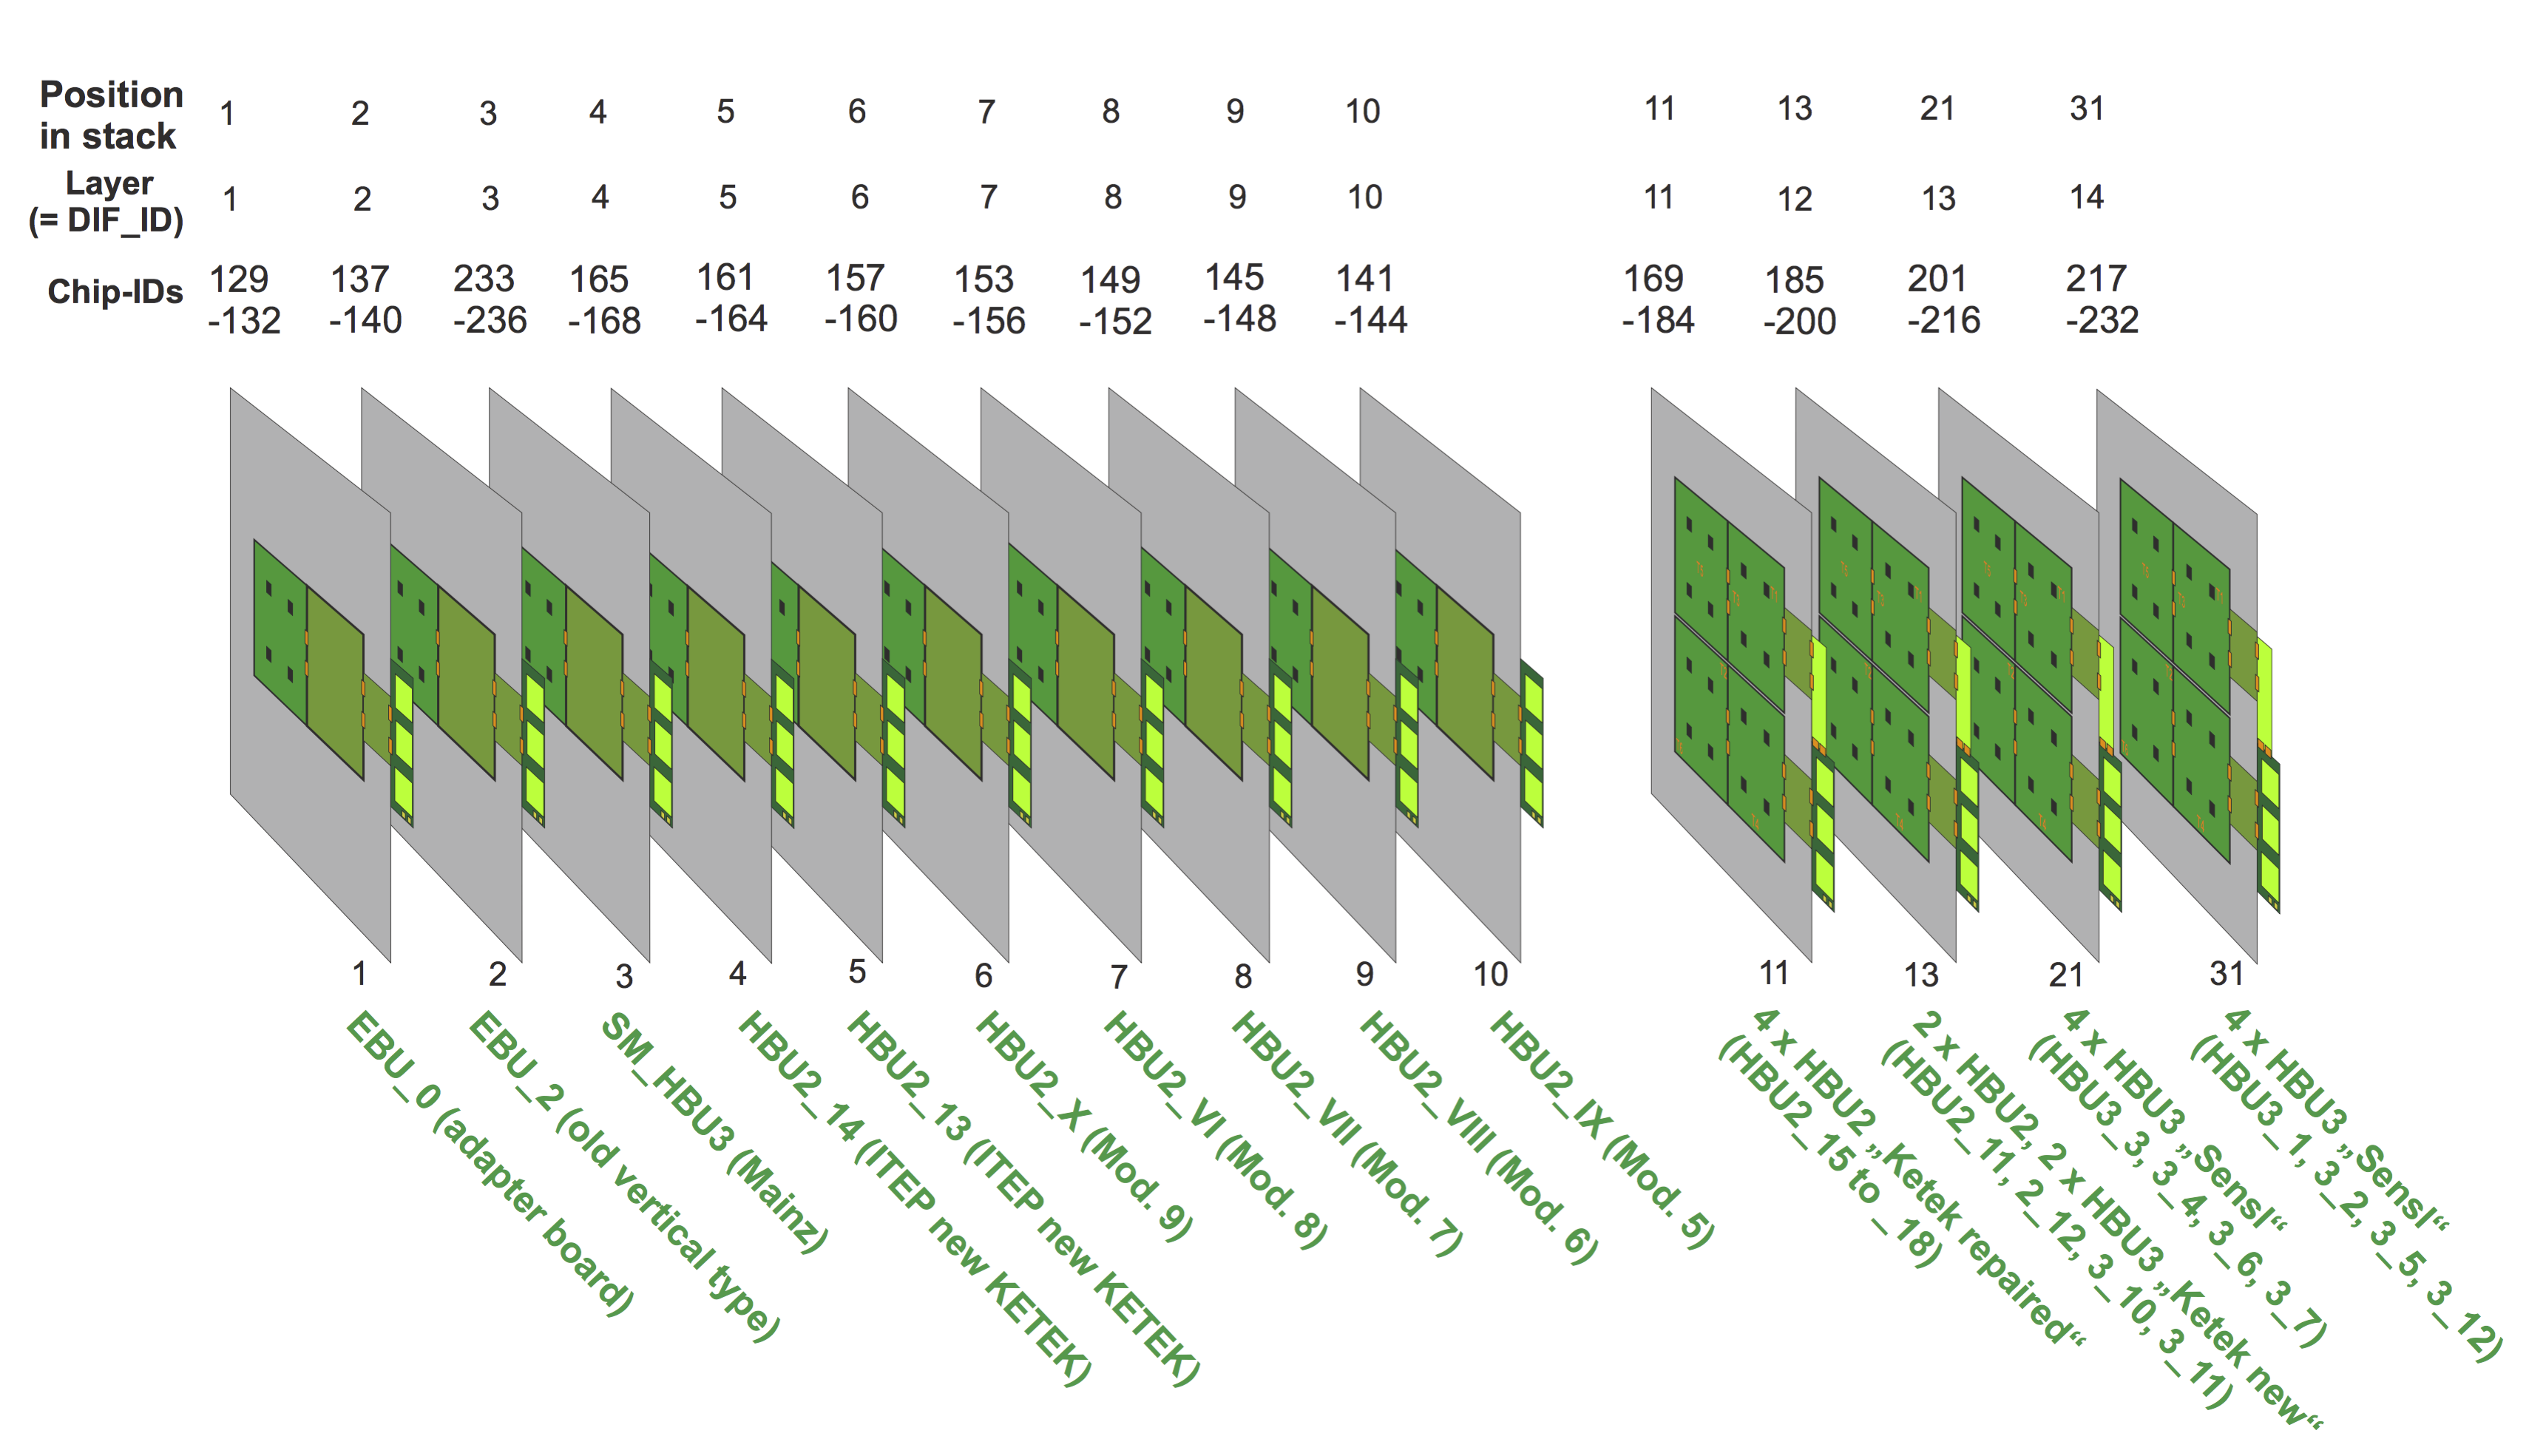
\includegraphics[width=0.60\textwidth]{fig/Detector_layout.png}}
	\caption[]{\textbf{a}: Picture of the CALICE AHCAL during the Testbeam in July 2015 at CERN. The trigger scintillators can be seen in front of the stack in the photo. \textbf{b}: Layout used during the July 2015 SPS Testbeam campaign.}
	\label{fig:full_detector_layout}
\end{figure}

\subsection{Testbeam Setup}

The two first layers consisted of ECAL Base Unit (EBU) with 144 scintillator strips of $45\times5\times2$ mm$^3$ read out by SiPMs for a total area of $18\times18$ cm$^2$. The next 8 layers consisted of a single HBU that can be used as a shower start finder in order to locate the first hard hadronic interaction. And the last 4 layers consisted of $2\times2$ HBUs in order to study timing of hadronic showers. The prototype was equipped by various SiPM types and tile designs that are summed up in table \ref{table:sipm_list}. The total number of channels is of 3744.
\begin{table}[h!]
\centering
\resizebox{\textwidth}{!}{%
	\begin{tabular}{cccccccc}
	\hline
    Layer\# & Producer & Model & Area (mm$^2$) & Pitch ($\mu$m) & WLS Fibre & Read out & Slot\\ 
    \hline
    1 & Hamamatsu & S12571\_010P & $1\times1$ & 10 & no & Bottom & 1\\ 
    2 & Hamamatsu & S10362-11-025O & $1\times1$ & 25 & no & Side & 2\\
    3 & Hamamatsu & S12571-025P & $1\times1$ & 25 & no & SMD & 3\\ 
    4-5 & Ketek & N/A & $2.25\times2.25$ & 18 & no & Side & 4-5\\
    6-10 & CPTA & CPTA & $1.28\times1.28$ & 40 & yes & Side & 6-10\\ 
    11-12 & Ketek & PM1125NS-SB0 & $1.2\times1.2$ & 25 & no & Side & 11-13\\
    13-14 & SenSL & MicroFB-10020-SMT & $1\times1$ & 20 & no & Side & 21-31\\
    \hline
    \end{tabular}
    }
\caption{List of the different SiPMs used in the CALICE AHCAL in July 2015.}
\label{table:sipm_list}
\end{table}

\subsection{The SPIROC2b chip}

The SiPMs are read out by a SPIROC2b chip which features 36 channels measuring ADC amplitudes (energy) and TDC amplitudes (time) and can store up to 16 events. The collected charge from the SiPM is stored in a capacitor (memory-cell) waiting to be digitised with a 12 bit range. The chip can be configured in 2 different modes. External trigger mode is used for gain calibration via an integrated LED Calibration System and monitoring of the SiPM. Auto-trigger mode is used to collect physics data. A threshold between 0.2-0.5 MIP is set for each chip in the setup. The amplitude signal amplified by a pre-amplifier with two different gains (High Gain and Low Gain) and then is measured via a slow shaper (50 ns shaping time) before being stored into a memory cell. The time is measured via a fast shaper (15 ns shaping time) when the signal passes the threshold and is digitised by a voltage ramp. Each chip possesses two voltage ramps that are multiplexed when a new Bunch Crossing (BXID) occurs. The length of a BXID is defined by the slow clock of the chip. In testbeam, the clock used is of 250 kHz which would correspond to a BXID length of 4 $\mu$s but due to the ramp multiplexer a dead time of around 2\% has to be taken into account. Thus the ramp length is 3.92 $\mu$s \cite{EldwanSSP}. For testbeam operation, a validation signal coming from scintillator beam triggers can be provided to the chip in order to suppress noise hits \cite{DAQ}.\\
\begin{figure}[htbp]
\begin{center}
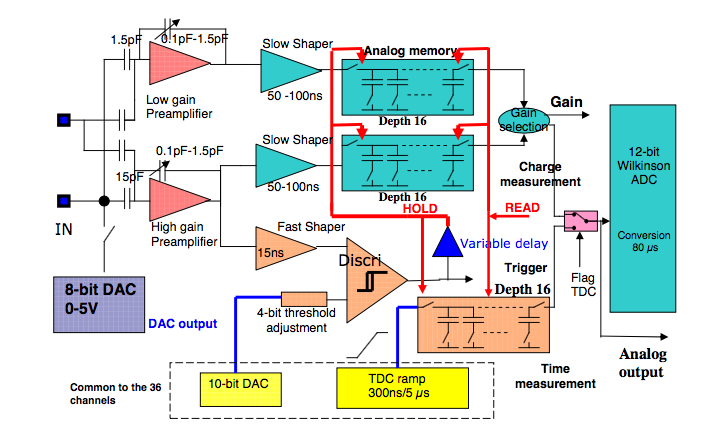
\includegraphics[width=0.6\textwidth]{fig/Spiroc_layout.png}
\caption{Schematic of the signal path of the SPIROC2B for a single channel \cite{SPIROCManual}.}
\label{fig:SPIROC2B}
\end{center}
\end{figure}

\subsection{Trigger Signals}
\label{subsec:trigger}

For Muon beam, two scintillator plates of $80\times80$ cm$^2$ were placed in front and back of the calorimeter. For electron and pion beams, two small scintillator plates of $30\times30$ cm$^2$ were positioned in front of the calorimeter (see figure \ref{fig:stack_steel}). The trigger scintillators were connected to a NIM-logic (discriminator and gate) in order to provide a validation of the data to the chip. 
In order to provide the time reference of the triggers, a SiPM-like pulse of around 4 $\mu$s length and with a fast rising edge around 1 ns was generated from the NIM-logic. This signal was injected directly via AC coupling to some channels in the setup as shown in the table \ref{table:trigger_signal_list}. No other external time reference than these channels is available.
\begin{table}[htbp]
\centering
  \begin{tabular}{@{} ccccc @{}}
    \hline
    Layer \# & Chip Number & Channel & Comments & Appellation \\ 
    \hline
    11 & 169 & 29 & noisy & T$_{11}$ \\ 
    11 & 177 & 23 & broken & - \\
    12 & 185 & 29 & - & T$_{12}$ \\ 
    13 & 201 & 29 & -  & T$_{13}$ \\
    13 & 211 & 6 & broken & - \\ 
    14 & 217 & 23 & - & T$_{14}$ \\
    \hline
  \end{tabular}
  \caption{List of channels with the injected trigger signal to be used as time reference.}
  \label{table:trigger_signal_list}
\end{table}
In the following analysis, only the reference signals T$_{12}$,  T$_{13}$ and T$_{14}$ were used.

\subsection{Dataset}
\label{subsec:dataset}

During the campaign at SPS in July 2015, $\mu^-$ runs were taken at 50 and 150 GeV beam energy for the calibration of the detector. Several e$^{-}$ runs were taken between 10 to 50 GeV beam energy to study the electromagnetic response of the calorimeter. The e$^{-}$ runs were quite pure as the beam was generated via a neutral beam directed on a converter target. Due to the significant amount of air and beam line instrumentation between the calorimeter and the final momentum selection magnet as well as few information of the beam parameters, the beam profile of electron runs is not well reproduce in simulation. Finally, $\pi^-$ runs were taken between 10 to 90 GeV beam energy. The table \ref{table:dataruns} sums up the dataset taken:
\begin{table}[htbp]
\centering
  \begin{tabular}{@{}l||p{2cm}p{8cm}@{}}
    \hline
    \multicolumn{1}{l}{\textbf{Particle}} & \textbf{Energy} & \textbf{Runs}\\
    \hline
    \multirow{2}{*}{$\mu^-$}& 50 GeV & 24016-24204\\& 150 GeV & 24623-24662\\
    \hline
    \multirow{2}{*}{e$^-$}& 10 GeV & 24531-24576\\& 15 GeV & 24507-24527\\& 20 GeV & 24479-24504\\& 30 GeV & 24454-24475\\& 40 GeV & 24420-24448\\& 50 GeV & 24404-24419\\
    \hline
    \multirow{2}{*}{$\pi^-$}& 10 GeV & 24266-24272, 24300-24317, 24381-24397\\& 20 GeV & 24398-24400\\& 30 GeV & 24259-24299, 24319-24380\\& 50 GeV & 24212-24254, 24325-24357, 24580-24612\\& 70 GeV & 24219-24242, 24365-24374\\& 90 GeV & 24233-24287, 24331-24364\\
    \hline
    \end{tabular}
  \caption{List of runs taken at SPS in July 2015.}
  \label{table:dataruns}
\end{table}

\section{Simulation}

\subsection{AHCAL Simulation Model \& Digitisation}

The simulation of the testbeam prototype is based on the \mokka framework v08-05-01 and the new \ddhep framework v00-16, which both provide a full \geant v10-1 based simulation of the detector implementations with detailed geometry and material descriptions. The right handed coordinate is used such as the Z-axis points in the beam direction and that the Y-axis is directed upwards. No beamline instrumentation is simulated except scintillator triggers in front and back of the detector. An additional layer of 5.6 mm of lead is added in front of the calorimeter in order to account for missing upstream material. This analysis uses the sub-detector \mokka models \textit{TBecal4d} for the ScECAL (Scintillator strips with EBUs) and \textit{TBhcal4d} for the AHCAL. The distance between the sub-detectors is set to 0 mm. A check was performed between \mokka and \ddhep models with electrons and pions to ensure that the material description in both models are approximately the same.\\
The beam gun is placed 1 m in front of the calorimeter face for the simulations in this analysis. It is configured to generate single beam particle with a 2\% momentum spread (according to the beamline) and the beam profile for electrons and pions is extracted from data and applied to simulation. For muon runs, a flat beam covering the full AHCAL is simulated as this is not expected to have an influence on the MIP and time response of the detector.
All electron simulations are simulated with \geant 10.1 using the QGSP\_BERT\_HP physics list.\\
Pion showers are simulated using QGSP\_BERT, QGSP\_BERT\_HP and FTFP\_BERT\_HP physics lists as theses physics lists are well validated for the simulation of high energy showers in steel-scintillator sandwich calorimeter \cite{AHCAL_Physics}. The package \textit{high precision} (\_HP) is used in order to understand the differences induced in timing with a precise treatment of the neutrons.\\
For each energies, 100 000 simulated $\mu^-$, $e^-$ and 200000 $\pi^-$ single particle events are generated.\\

The digitisation of simulated hits is very similar to the one used in the ScECAL and AHCAL physics prototypes \cite{CAN-002, CAN-010, JINST-6}. Using, if available, individual calibration factors obtained from data to extract the light yield which is needed to model the statistical fluctuations of photons hitting a SiPM. Saturation effects are also included using the number of pixels available on each SiPM type. Most of the tiles used are wrapped with a reflective foil in order that crosstalk effect between channels can be neglected. For layers with no wrapping a default value of 15\% cross-talk is applied. The timing is modelled in the same way as in the SPIROC, the energy from sub-hits in a cell is integrated over a sliding time window of 15 ns, if the energy sum passes the threshold the time of the simulated sub-hit passing the threshold is registered as the time of the hit. In order to simulate detector resolution effects, the time of a hit is smeared with a double gaussian function with slightly different means and sigmas convoluted with a gaussian of fixed mean (at 0) and variable sigma explained in section \ref{}. Noise needs to be taken into account for with the engineering AHCAL prototype as only hits above the trigger threshold are registered during a beam spill. A study of the effect of noise on timing is described in appendix \ref{appendix:noise_timing}.\\
After digitisation, simulated hits have the same format as raw data hits and are then reconstructed using the same software chain used for data. To suppress noise hits, only hits above 0.5 MIP are considered in this analysis in both simulation and data.

\section{Timing Calibration}

To perform the timing calibration of the AHCAL, the complete muon dataset is used. The electron dataset is used in a next step to validate the calibration procedure as described in subsection \ref{subsec:validation}. Table \ref{table:mu_elec_runs} summarises the runs and datasets used. The number of raw events are counted if containing all the three trigger signals.
\begin{table}[htbp]
\centering
  \begin{tabular}{@{} cccccc @{}}
    \hline
    Runs & Energy & Particle Type & Events (raw) & Events (sel.) & $\frac{\text{N$_{sel.}$}}{\text{N$_{raw}$}}$ \\ 
    \hline
     24016-24663 & 50-150 GeV & $\mu^-$ & 990161 & 660662 & 66.7\% \\ 
     24486-24504 & 20 GeV & $e^-$ & XXXX & XXXX & 85.9\% \\
    \hline
  \end{tabular}
  \caption{Table with the statistic before and after selection used for timing calibration.}
  \label{table:mu_elec_runs}
\end{table}

\subsection{Muon Selection}

The $\mu$ runs were taken first at 50 GeV then another scan at the end of the campaign was performed at 150 GeV. The muon beam was produced by scrapping the halo of a secondary pion beam using collimators. The muon runs were contaminated by pions, a first estimation provided that around 30\% of the events were contaminated. The main goal of the muon selection was to efficiently select muons and reject pion showers. For this, a simple track finder has been developed. In order to select muons or punch-through pions, a straight track of at least 7 hits is required in the whole AHCAL without a hard interaction. In addition to reject late pion showers, not more than 2 hits are required per layer.

\subsection{Slope calibration}
\label{subsec:slope_calib}

The data analysis is performed in several steps. The first step is the calibration of the time provided by the SPIROC2B chip. To reconstruct the time of the first hit (only single hit per channel is registered during a bunch-crossing) in a channel, the TDC value measured needs to be converted into nanoseconds. The value is converted using the following equation:
\begin{equation} \label{eq:slope}
 \text{slope}_{chip, BXID} \: \text{[ns/TDC]} = \frac{3920 \: \text{ns}}{\text{Max}_{chip, BXID} - \text{Pedestal}_{chip, BXID}}
\end{equation}
\begin{equation} \label{eq:time_chn}
\text{T}_{chn} \: \text{[ns]} = \text{slope}_{chip, BXID} \times (\text{TDC} - \text{Pedestal}_{mem=1} )
\end{equation}
The determination of the parameter $\text{slope}_{chip, BXID}$ is assuming that the TDC ramp is linear. The parameters Max$_{chip, BXID}$ and Pedestal$_{chip, BXID}$ in eq.\ref{eq:slope} are extracted from the TDC spectrum from a specific chip and BXID using only the first memory cell as illustrated in figure \ref{fig:TDC_Spectrum}. At the same time, the parameter Pedestal$_{mem=1}$ in eq.\ref{eq:time_chn} is extracted from the spectrum for each channel and the first memory cell of a chip without taking into account the BXID of the ramp as the difference between both pedestal can be corrected for at a later stage. This is accounting for a total of 208 slopes and 3744 pedestals to be extracted for the testbeam setup.
\begin{figure}[htbp]
	\subfigure[TDC Spectrum of a typical chip.\label{fig:TDC_Spectrum}] {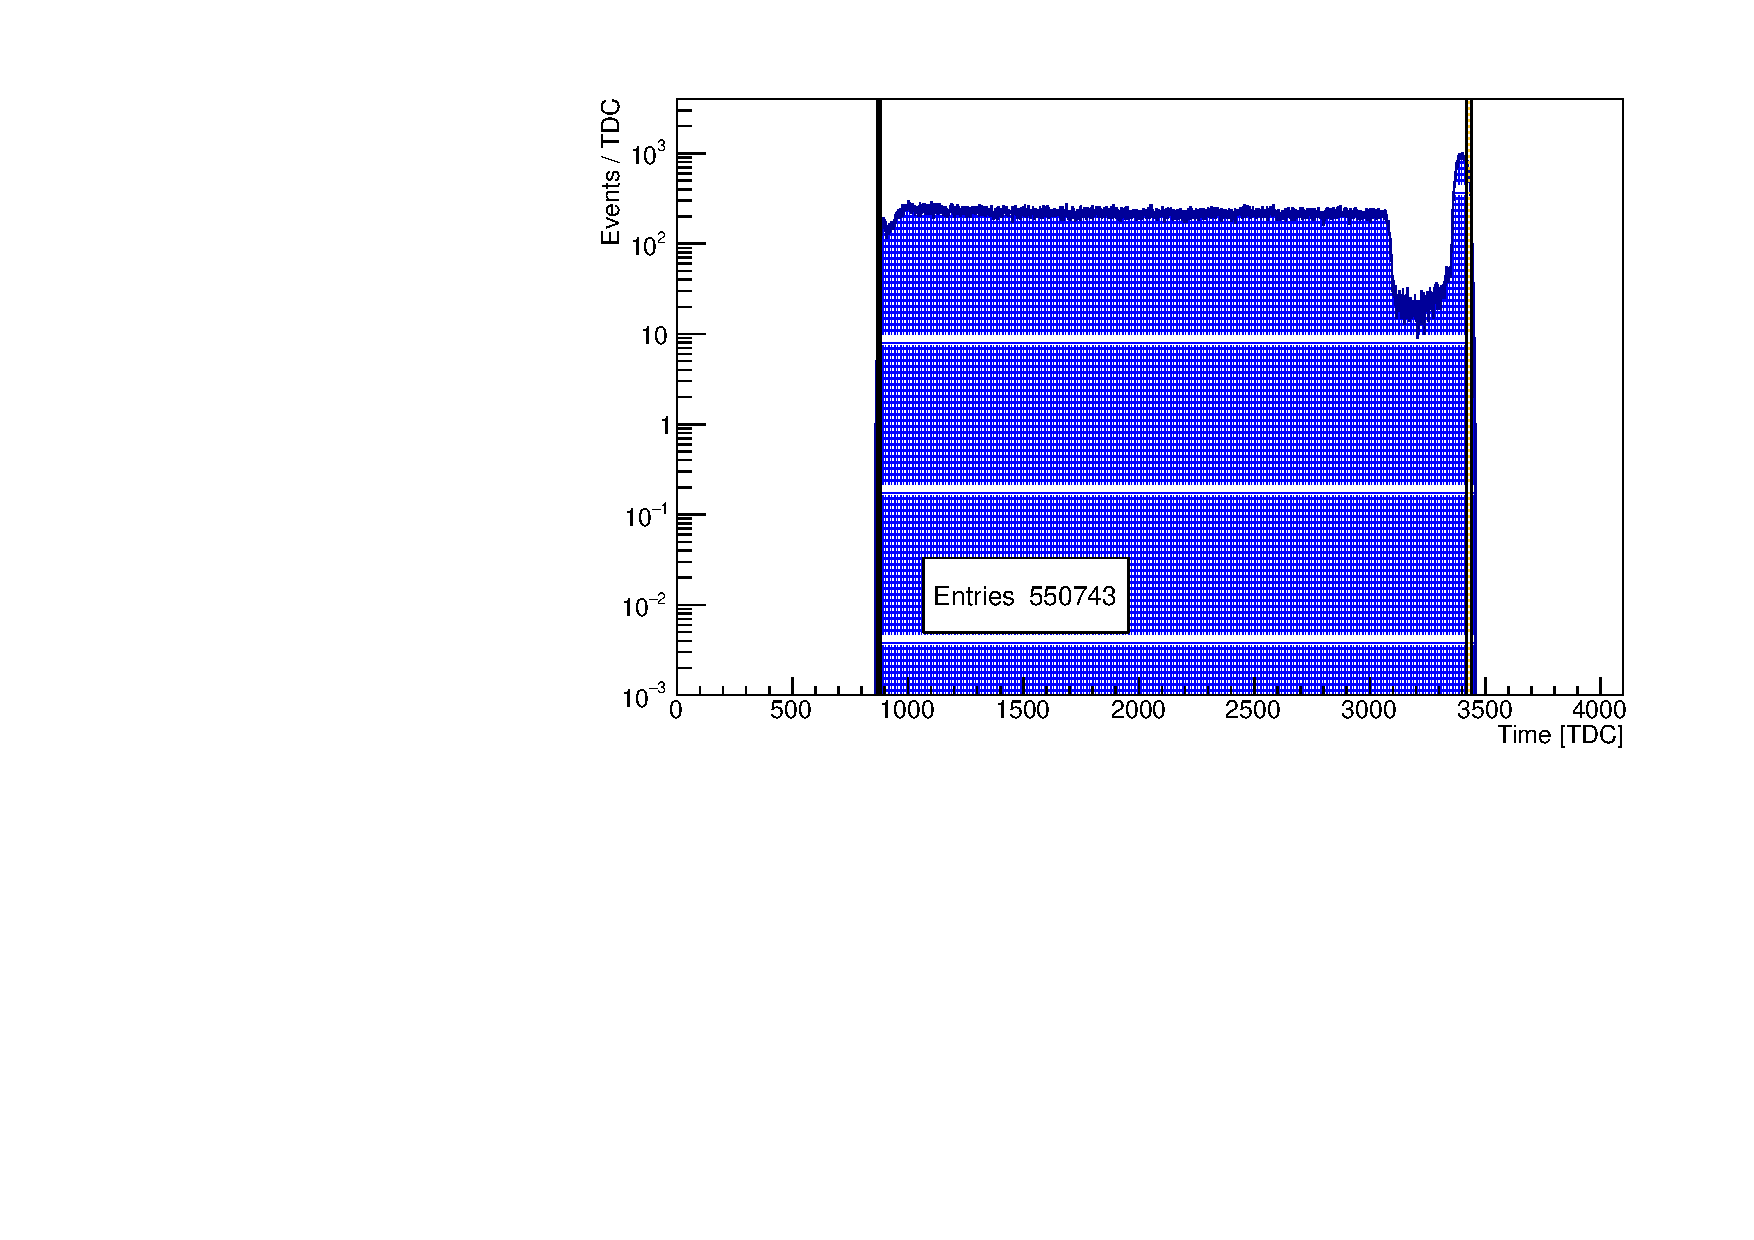
\includegraphics[width=0.5\textwidth]{fig/ExampleTDCSpectra.pdf}}\hfill
	\subfigure[Distribution of the fitted slopes for even and odd bunch-crossing IDs.\label{fig:slope_time}] {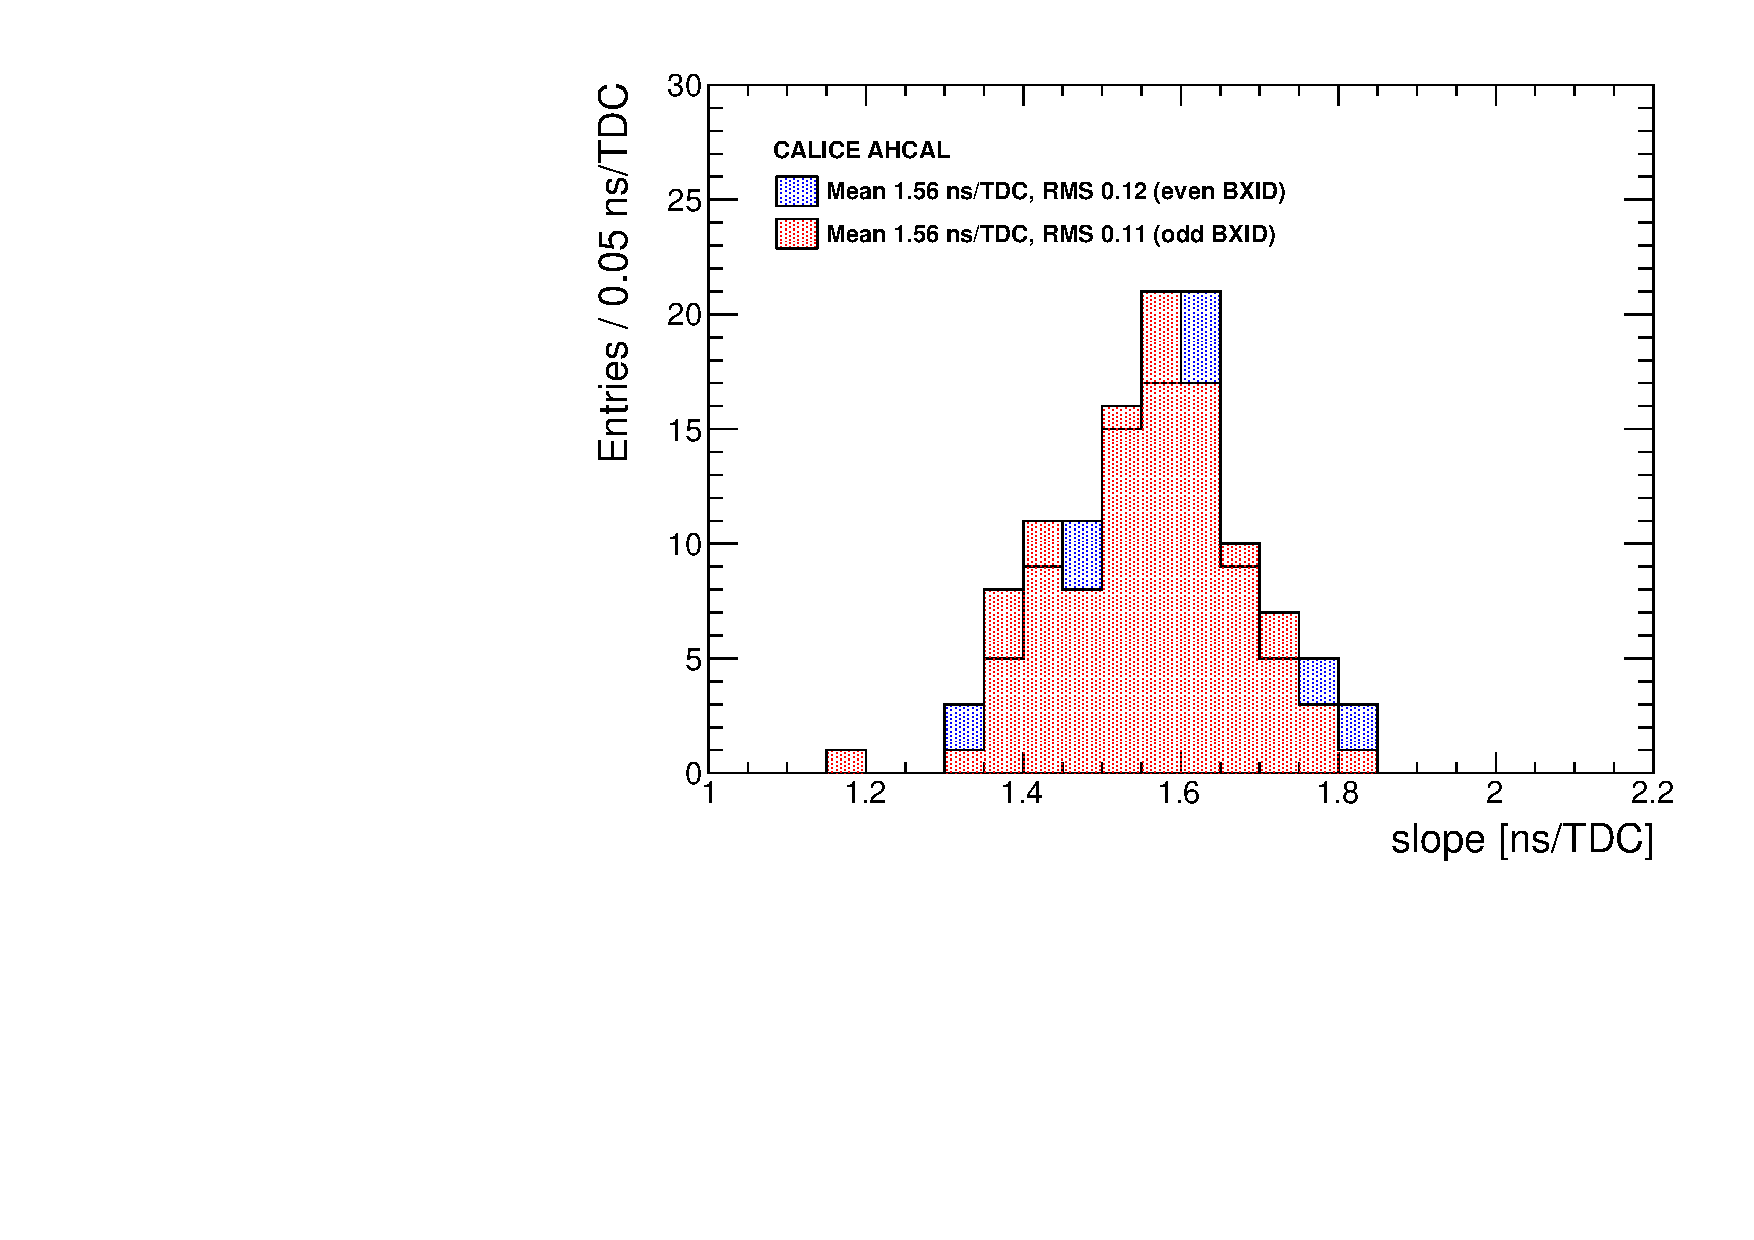
\includegraphics[width=0.5\textwidth]{fig/SlopesTDC.pdf}}
	\caption[]{\textbf{a}: The red rectangle are the fitted Max and Pedestal parameters for this chip. The yellow bands represents estimation of the error made on the extraction of the parameters by a variation of 1 RMS of the threshold $\mu$. The parameters extracted are slope = 1.56 $\pm$ 0.01, Pedestal = 816 $\pm$ 9 and Maximum = 3336 $\pm$ 8. \textbf{b}: $\mu_{odd}$ = 1.564 ns/TDC, RMS$_{odd}$ = 0.121, $\mu_{even}$ = 1.556 ns/TDC, RMS$_{even}$ = 0.113.}
\end{figure}
The technique of extraction is based on an edge detection method. For each chip and BXID, an histogram is filled with the y value of each bin then the mean of this histogram is defined as a threshold $\mu$. The parameter Pedestal$_{chip, BXID}$ is extracted as the first bin above 30\% of $\mu$. For the parameter Max$_{chip, BXID}$, it is extracted by taking 50\% of the maximum bin of the original histogram. An estimation of the errors made on the pedestal and maximum is done by looking at the maximum difference between 1 RMS of $\mu$ and 33\% of the maximum bin to the extracted value. The maximum seems not to be exactly at the last bin of the spectrum, this is due to the technique that needed to be robust against strange spectra like on figure \ref{fig:TDC_Spectrum_Layer11}.
The extracted values for the slopes are in the expected range of 1.6 ns per TDC bin due to the limited dynamic range provided by the chip (around 2500 bins for 4 $\mu$s). More details about the estimations of the calibration errors is described in the appendix \ref{appendix:calib_error}.

\subsection{Calibration of the reference time}

\subsubsection{Time reference}
To reconstruct the time of the first hit in a channel, the measured time of a hit needs to be compared to the time of the reference trigger. The trigger signals described in subsection \ref{subsec:trigger} are calibrated using the same method as explained above. After time calibration of the hit, events are selected by requiring that T$_{12}$, T$_{13}$ and T$_{14}$ are present in the event in a certain amplitude range to reject noise hits from theses channels. Moreover, as these channels receive exactly the same signal from the NIM-logic at the same time, a quadratic correction is applied to ensure that they match in time. The correction is performed by correcting the time of T$_{12}$ and T$_{13}$ compared to the time of T$_{14}$. The figure \ref{fig:T0_Correction} shows that the correction reduces the spread of the trigger channels w.r.t to each other. The resulting resolution for the reference trigger signal is around 4-5 ns, this resolution from the electronics contributes to the final timing resolution obtained.
\begin{figure}[htbp]
\begin{center}
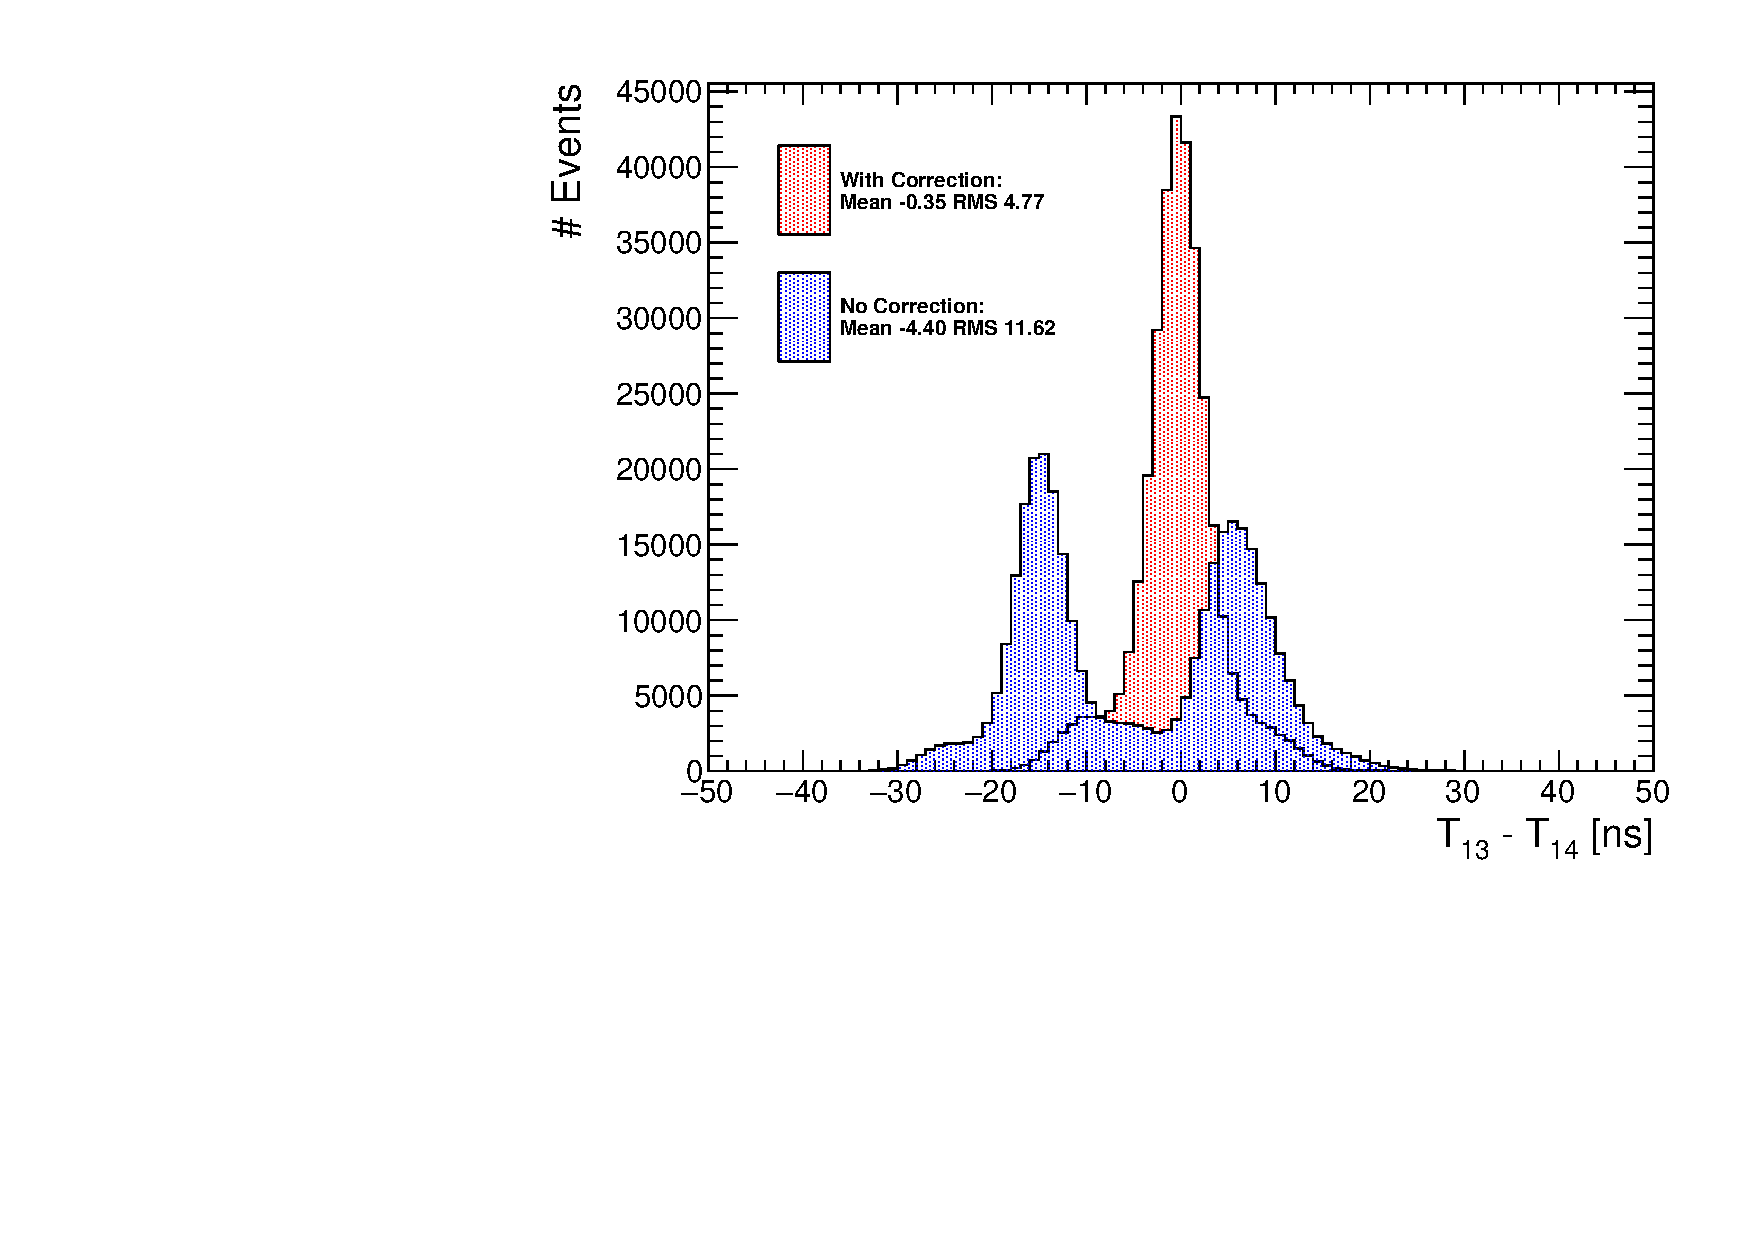
\includegraphics[width=0.6\textwidth]{fig/T0s/T0_Resolution_6.pdf}
\caption{Time difference between the trigger channels before and after correction for T$_{13}$ and T$_{14}$. The histogram in blue shows the difference between the channels before correction, the histogram in red shows the difference after correction. $\mu$ = -4.4 ns, RMS = 11.62 ns, $\mu_{corrected}$ = -0.35 ns, RMS$_{corrected}$ = 4.77 ns}
\label{fig:T0_Correction}
\end{center}
\end{figure}
In a next step, to reduce the uncertainty made on the time of the trigger, the time reference $T_{ref}$ is calculated using the mean of T$_{12}$, T$_{13}$ and T$_{14}$ and its associated error $\sigma_{ref}$ as shown in eq. \ref{eq:tref} \& \ref{eq:tref_err}. A cut of 4 ns is performed on $\sigma_{ref}$ to reject events with a too large error on the time of the trigger.
\begin{equation} \label{eq:tref}
\text{T}_{ref} = \frac{\text{T}_{12} + \text{T}_{13} + \text{T}_{14}}{3}
\end{equation}
\begin{equation} \label{eq:tref_err}
\sigma_{ref} = \frac{ (\text{T}_{12} - \text{T}_{ref})^2 + (\text{T}_{13} - \text{T}_{ref})^2  + (\text{T}_{14} - \text{T}_{ref})^2 }{6}
\end{equation}
Since the absolute time between the passage of a muon and the trigger of a channel is not known due to cabling and the trigger electronics, the time offset relative to the trigger is determined from data. Muons are quasi-instantaneous particles thus the time of the first hit distribution for each channel, memory cells and BXID has to be shifted to \textit{t=0}. This shifting procedure takes into account the delay time of the trigger due to cabling and the NIM-logic as well as mis-calibrations in memory cell pedestals. Only channels containing more than 100 events are considered. This offset is determined by iteration requiring at least 4 prompt hits i.e hits in the range from -20 to 20 ns of the event. In this way, 18338 individual offsets are extracted from data. A distribution of the extracted offsets using muon data can be seen in figure \ref{fig:offset_trigger_distribution}. The figure \ref{fig:BXID_offset} shows that individual offsets have to be extracted for each BXID as the correlation is chip-dependent and not the same for odd and even BXIDs.
\begin{figure}[htbp]
	\subfigure[Distribution of the offset used to correct for the trigger delay.\label{fig:offset_trigger_distribution}] {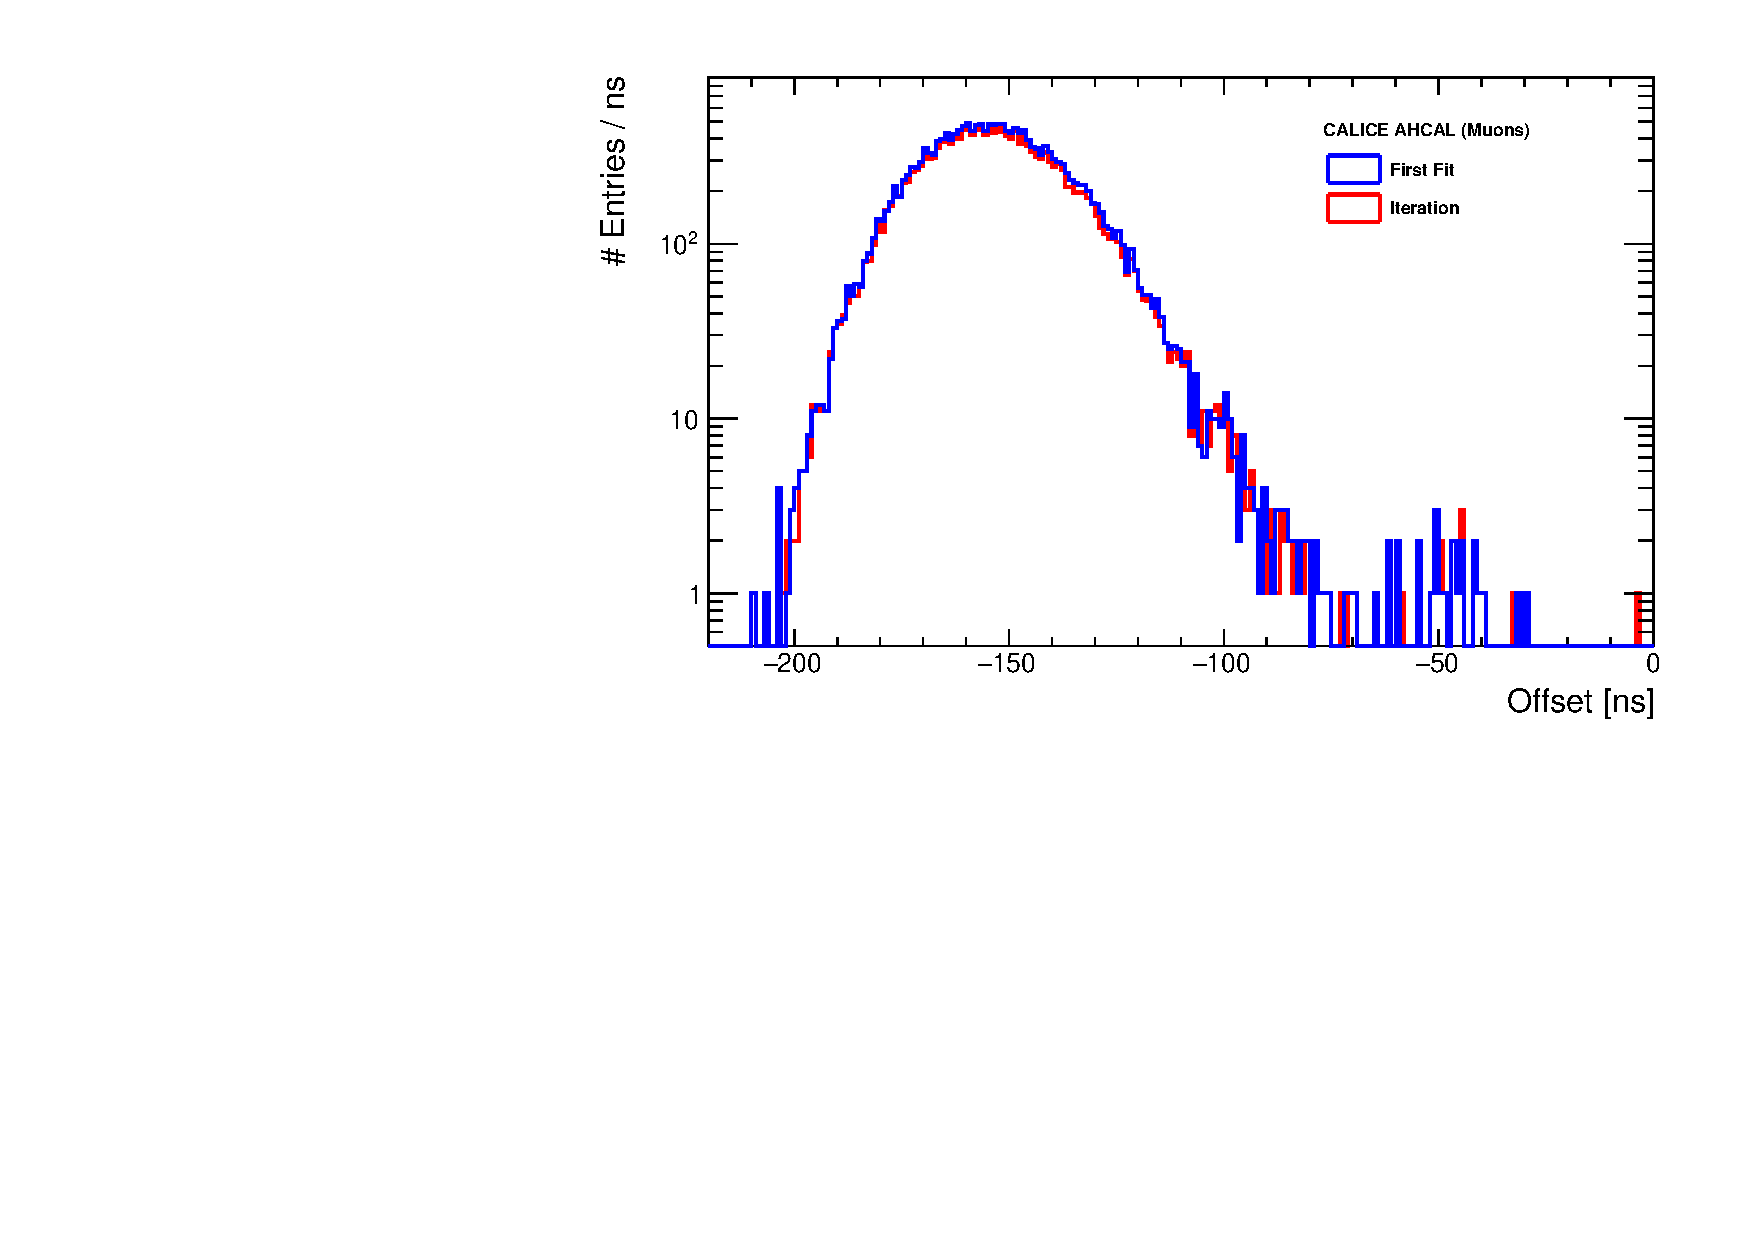
\includegraphics[width=0.5\textwidth]{fig/ExtractedOffsets.pdf}}\hfill
	\subfigure[Correlation between offsets extracted for even and odd BXID.\label{fig:BXID_offset}] {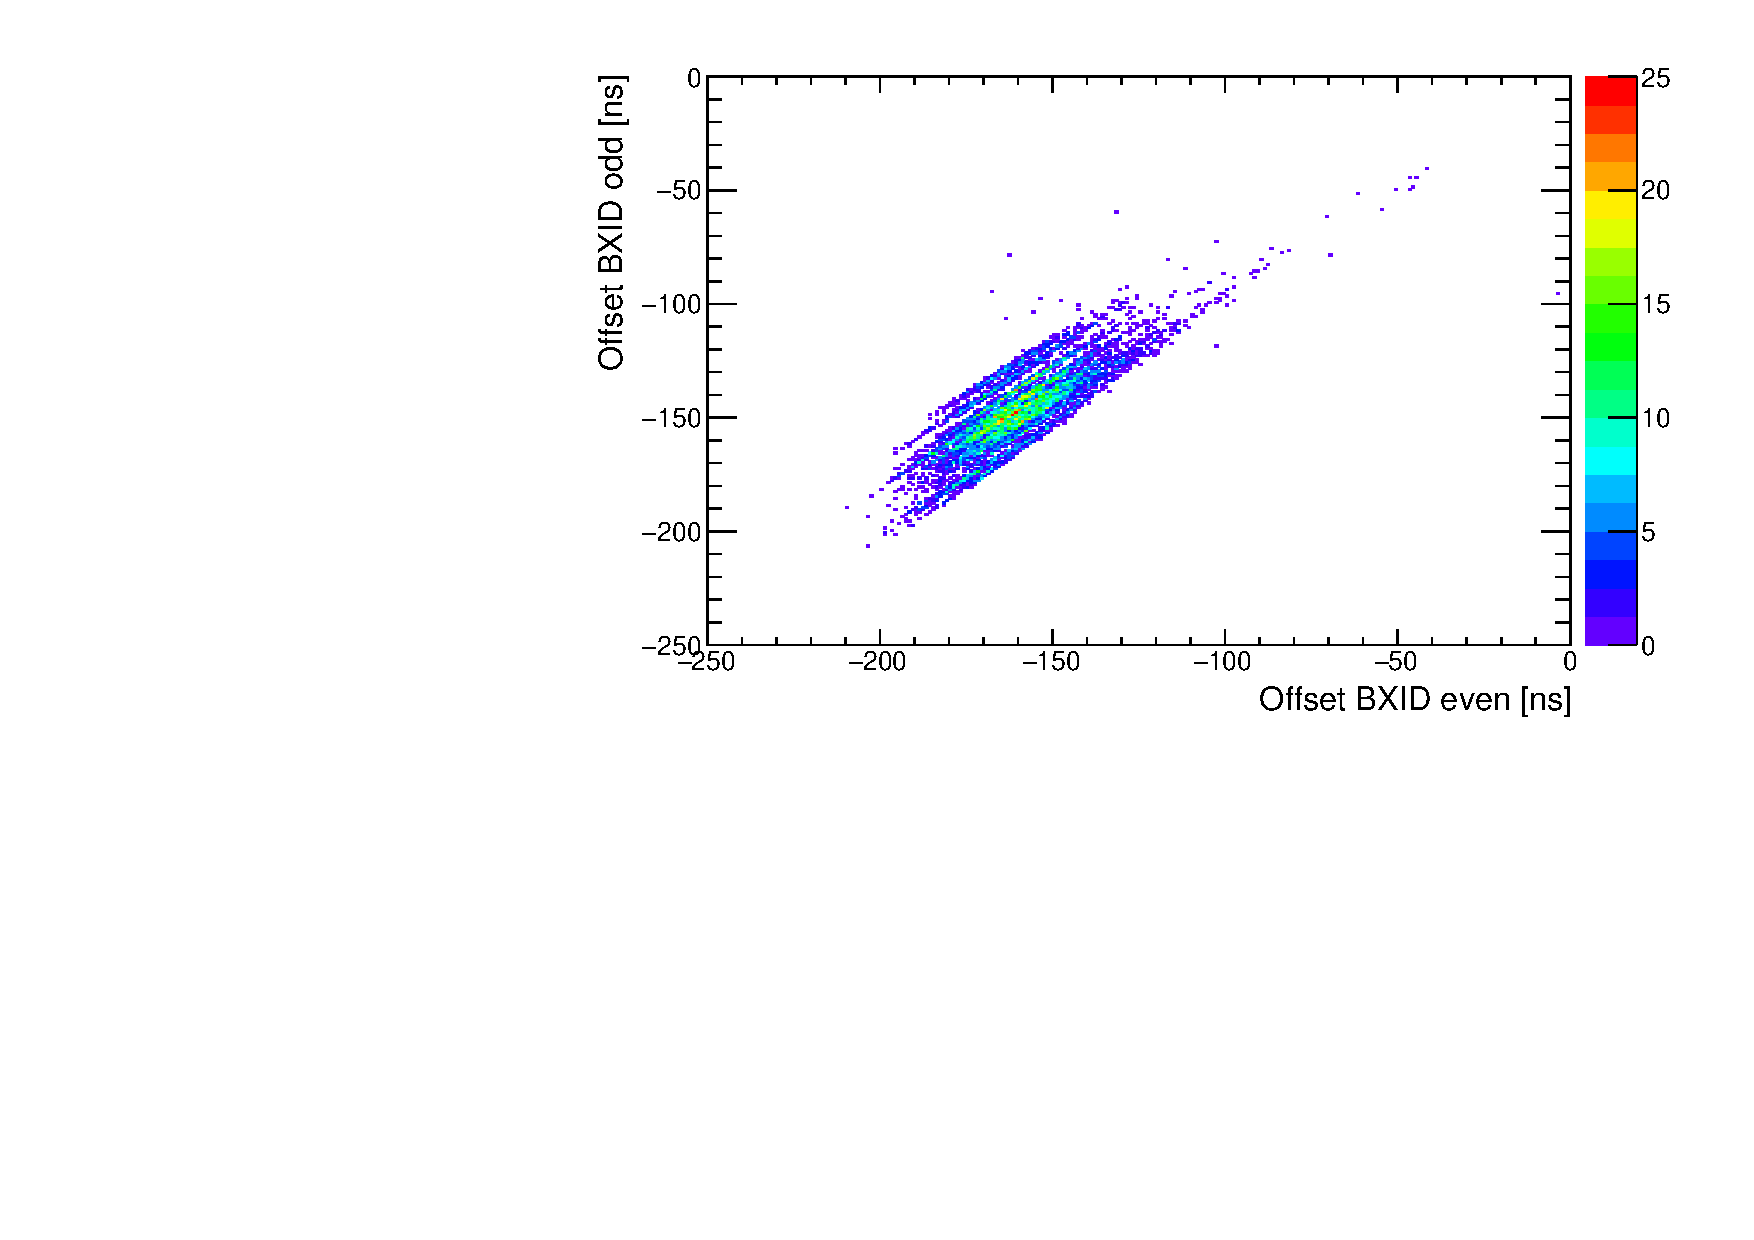
\includegraphics[width=0.5\textwidth]{fig/CorrelationOffsets_BXID.pdf}}\hfill
	\caption[]{\textbf{a}: Extracted offset used to correct for the trigger delay signal. The mean delay of the trigger is $\sim$150 ns. \textbf{b}: Correlation between offsets extracted for BXID even and odd. The correlation seems is not perfectly at 45 degrees explaining the need for individual offsets per BXID.}
\end{figure}

\subsubsection{Time of the first hit distribution}
After the selection, the time of the first hit (T$_{fH}$) can be obtained by plotting the distribution of T$_{chn}$ - T$_{ref}$ for each layer as shown in figure \ref{fig:layer3_timing_nocorrection}.
\begin{figure}[htbp]
	\subfigure[Timing for layer 3 in the AHCAL.\label{fig:layer3_timing_nocorrection}] {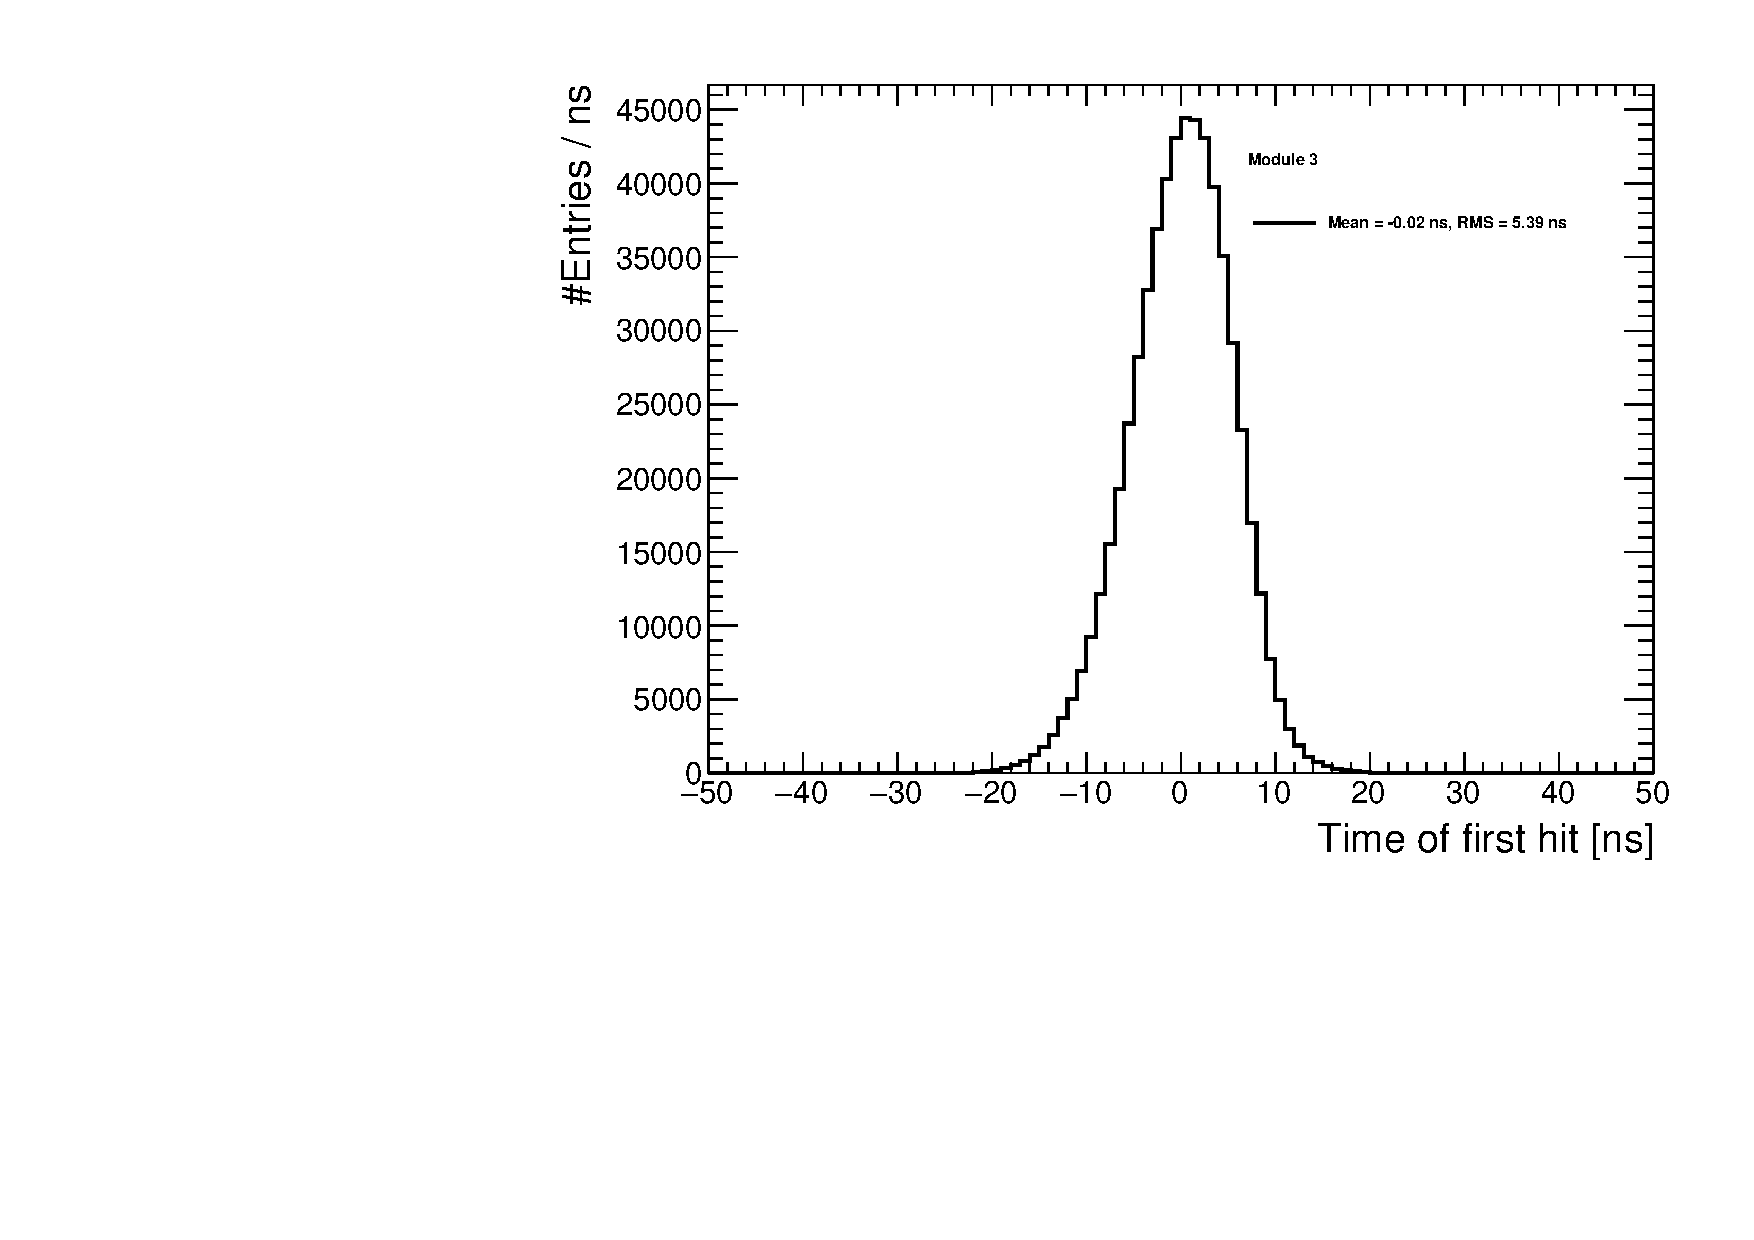
\includegraphics[width=0.5\textwidth]{fig/Muons_noCorrections/TimeDistribution_Module3.pdf}}\hfill
	\subfigure[Extracted resolution for all layers in the AHCAL.\label{fig:reso_nocorrection}] {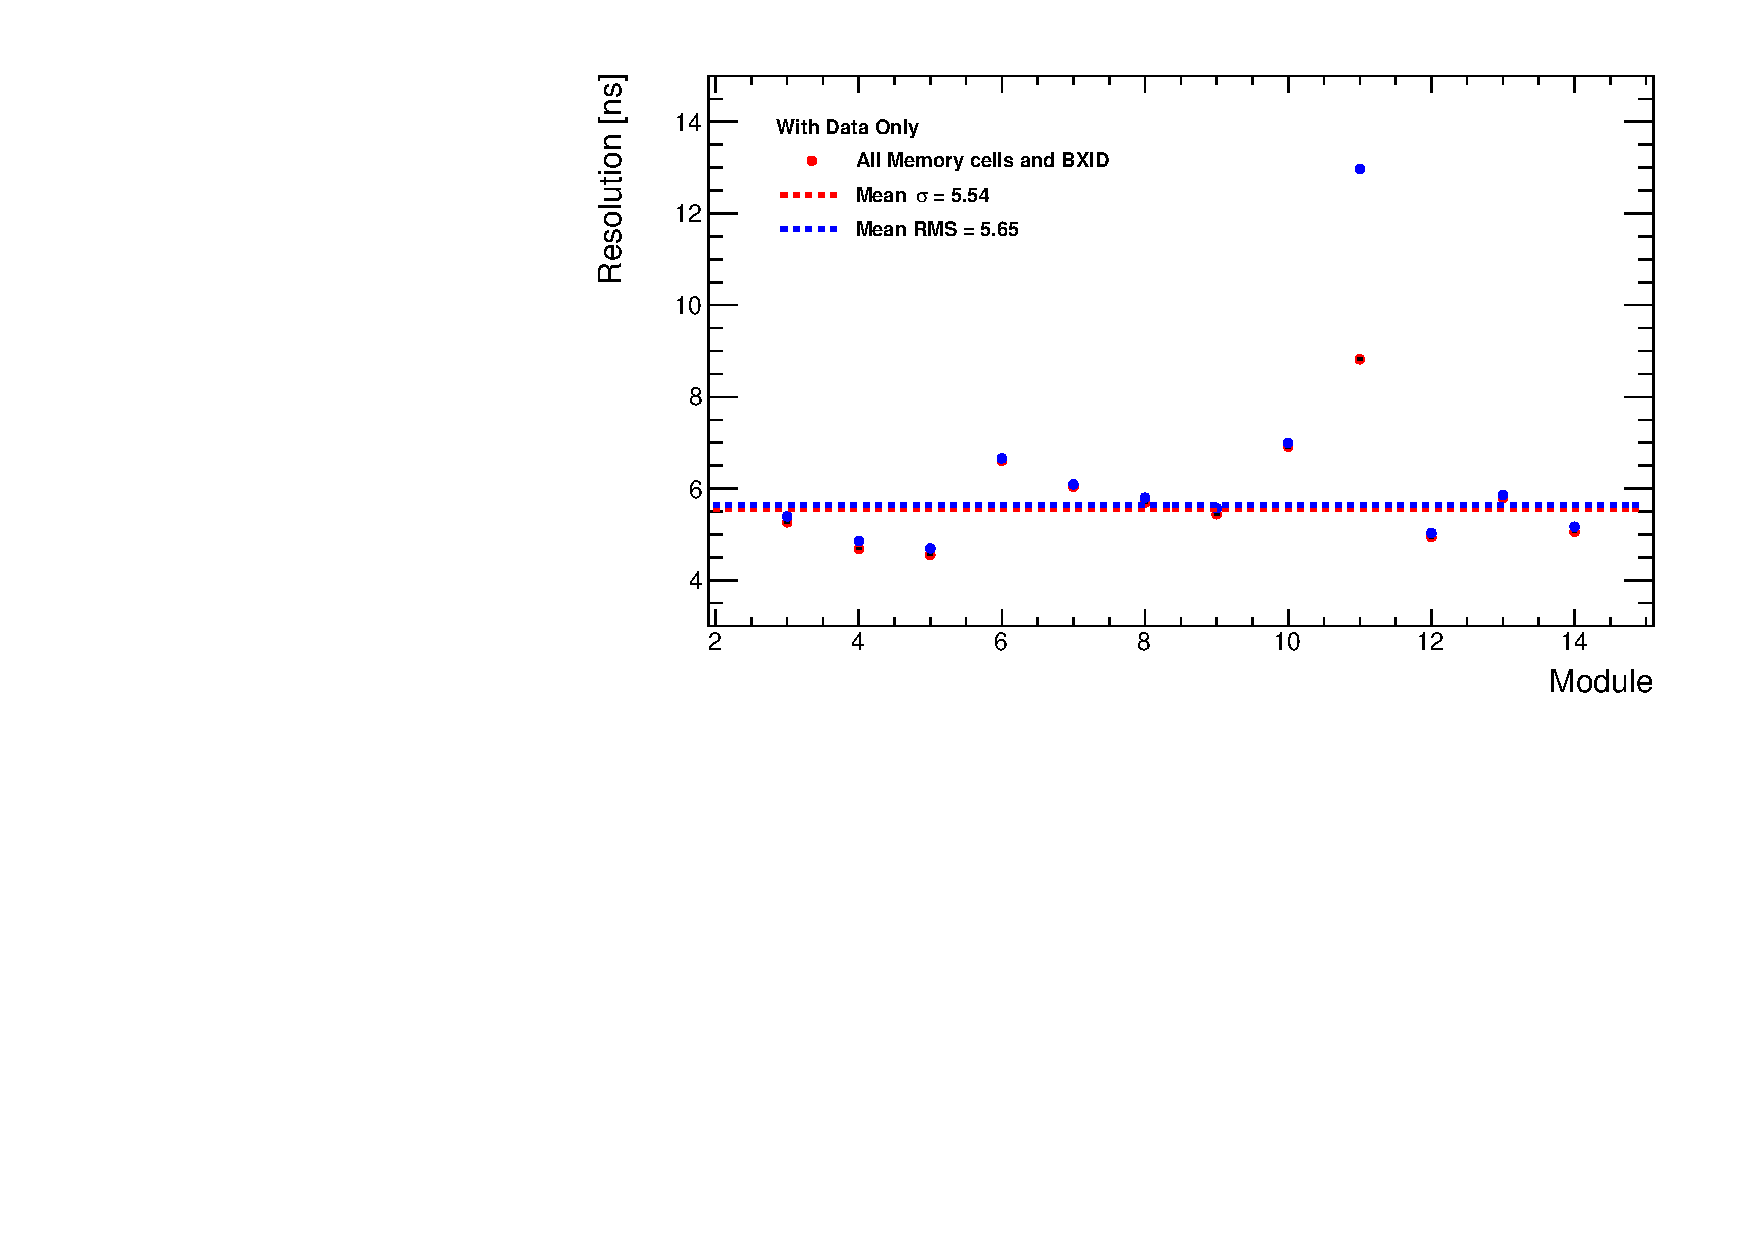
\includegraphics[width=0.5\textwidth]{fig/Muons_noCorrections/ResolutionPerModule.pdf}}\hfill
\caption[]{\textbf{a}: Time of the first hit distribution of the AHCAL in layer 3 after the first part of the calibration. $\mu$ = 0.02 ns , RMS = 5.39 ns. The distribution is clearly asymmetric. \textbf{b}: Time resolution for all layers in the AHCAL. The mean RMS is 5.65 ns.}
\end{figure}
The combined time resolution (RMS) shown in figure \ref{fig:reso_nocorrection} obtained by combining all layers is around 5.65 ns by just applying the time calibration on the data. Some improvements are possible as described in the subsections \ref{subsec:lin_corr} and \ref{subsec:timewalk}. The discrepancy observed for the layer 11 is most likely due to an electronic problem in the TDC voltage ramp of the chips on that layer.

\subsection{Corrections applied to data}
\subsubsection{Ramp non-linearity correction}
\label{subsec:lin_corr}

The calibration relies on the linearity of the TDC voltage ramp in the SPIROC2b by measuring the minimum and maximum of the ramp and interpolating assuming a linear ramp. This assumption is not entirely reliable as described in \cite{OskarSSP, EldwanSSP}. For this, a correction of the non-linearity has to be applied. By simply looking at the time of the first hit (T$_{fH}$) for each chip and BXID versus the TDC value of the hit, the shape of the graph would indicate how reliable is the assumption. Indeed if the ramp would be perfectly linear, one would obtain a flat graph.
A quadratic fit is performed for each chip and BXID in order to correct for the non-linearity of the ramp as shown on figure \ref{fig:LinCorr}. A check has been performed on the quality of the correction, seen on figure \ref{fig:LinCorr_2}.
\begin{figure}[htbp]
	\subfigure[Quadratic fit of chip 146 (BXID even) on layer 09.\label{fig:LinCorr}]{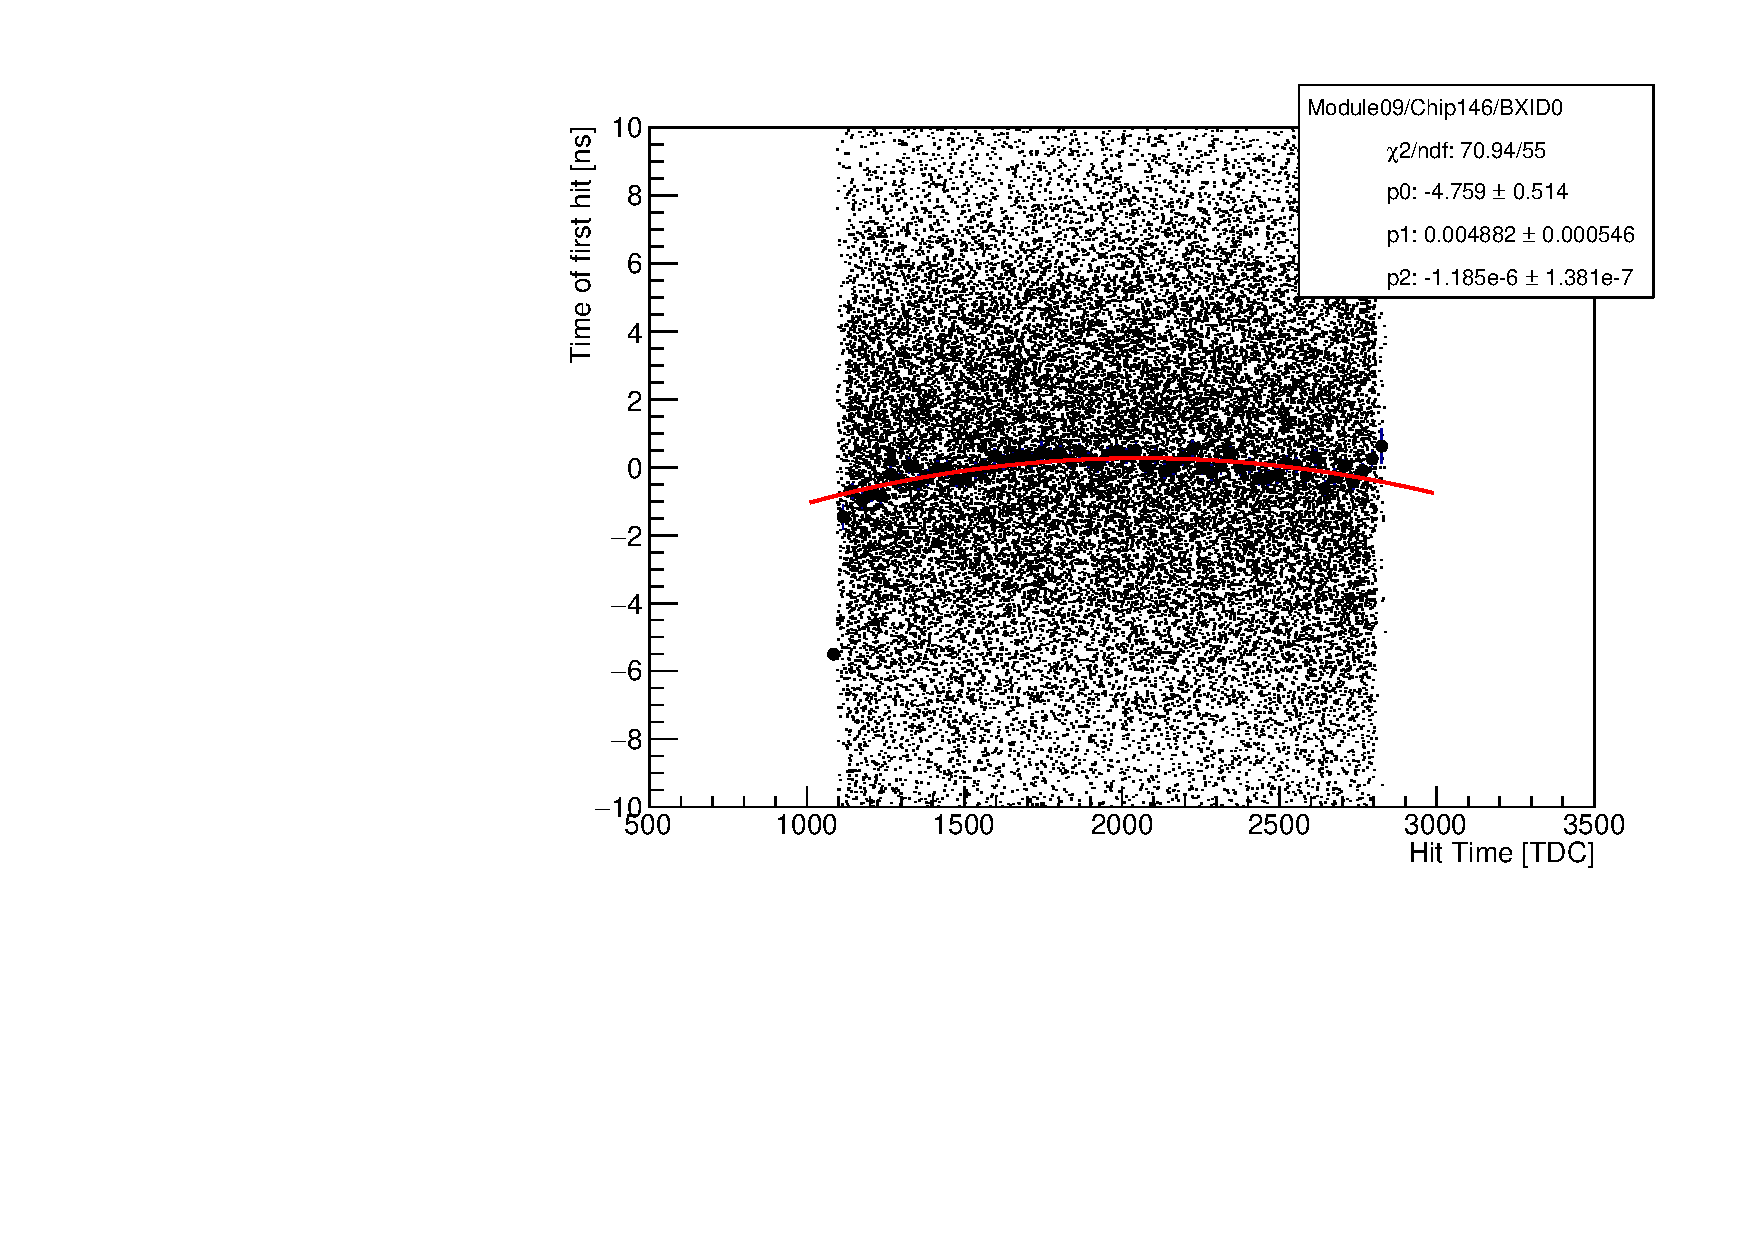
\includegraphics[width=0.5\textwidth]{fig/LinearityCorrection_Module09_Chip146_BXID0.pdf}}\hfill
	\subfigure[Profile for chip 146 on layer 09 after the non-linearity correction of the ramp.\label{fig:LinCorr_2}]{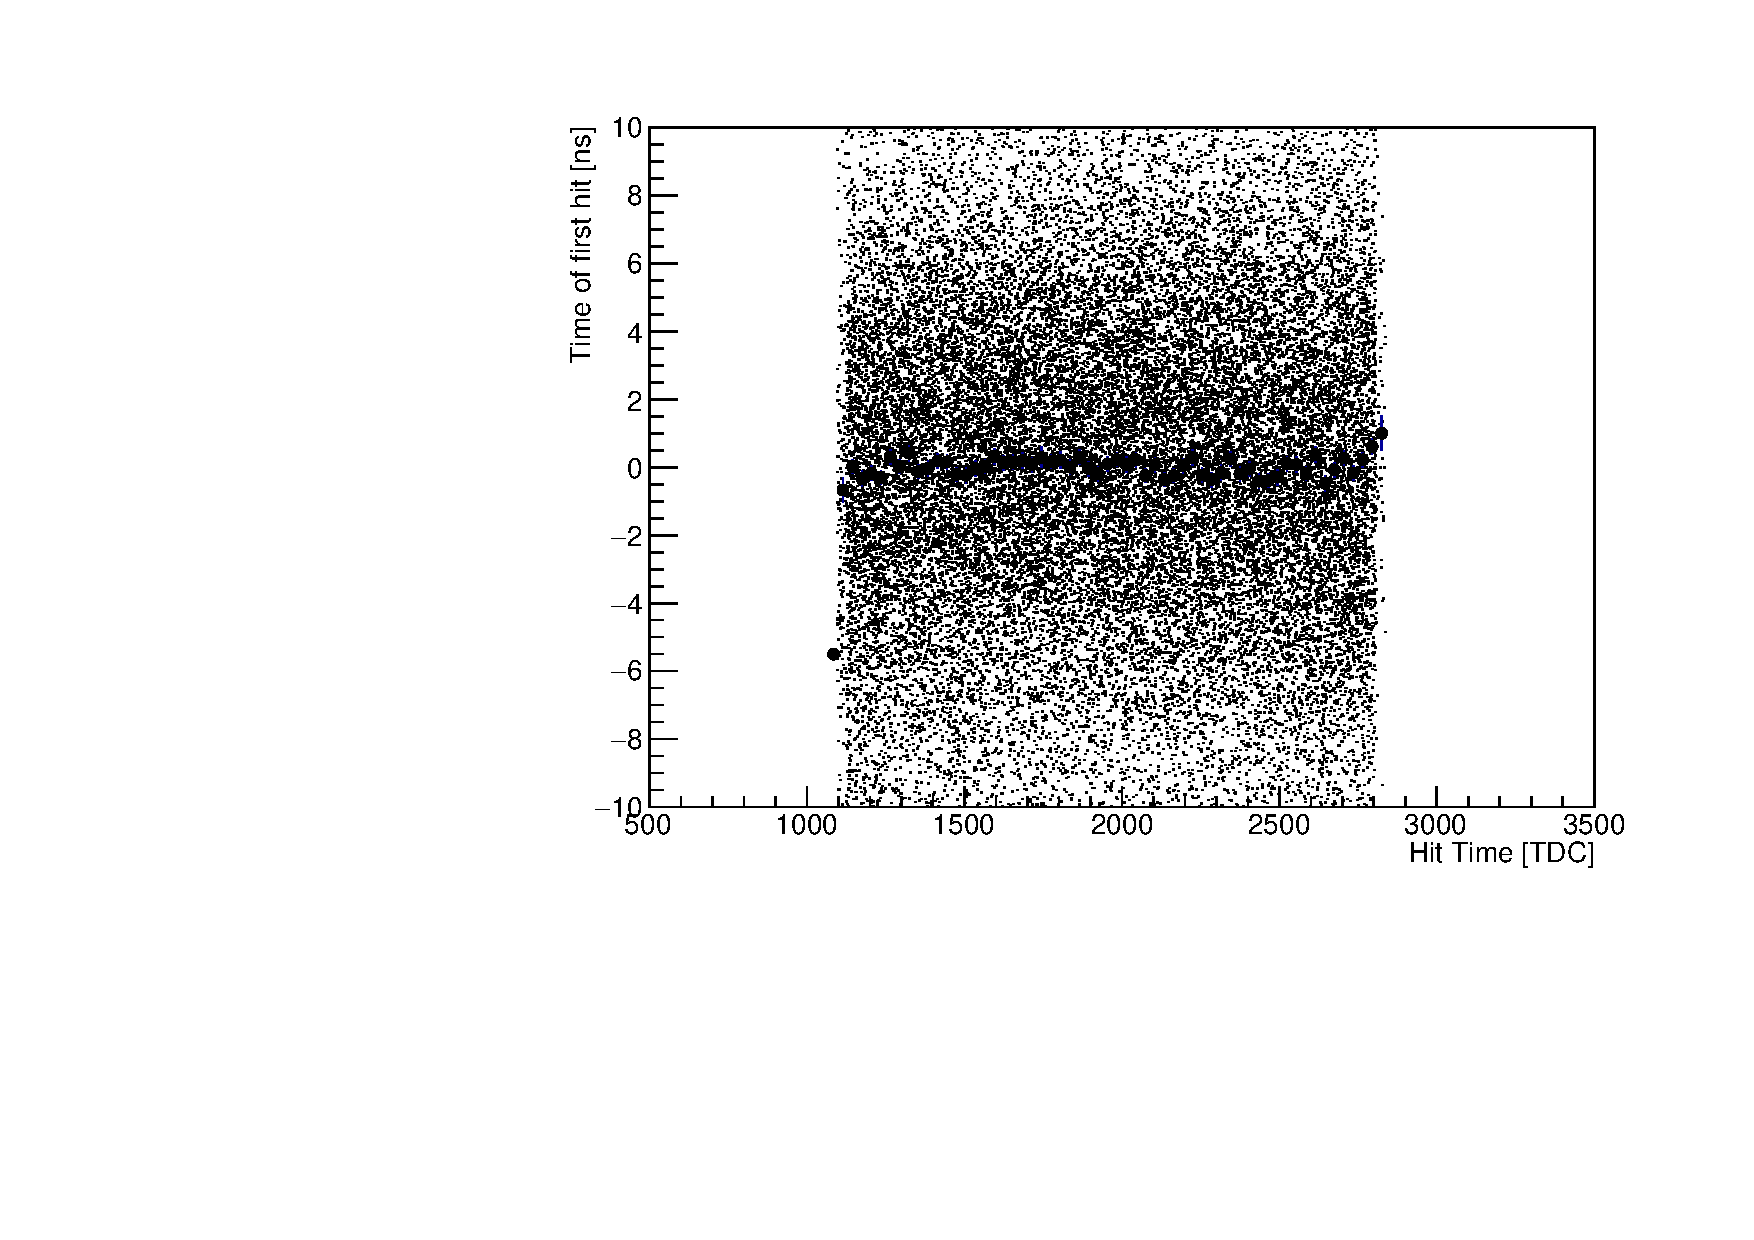
\includegraphics[width=0.5\textwidth]{fig/LinearityCorrection_Module09_Chip146_BXID0_Corrected.pdf}}
	\caption[]{\textbf{a}: The $\chi^2$ of the fit is 1.29. \textbf{b}: The correction parameter are applied then on the data to cross-check the quality of the correction. One can see that the curve flattens with the correction applied.}
\end{figure}
The non-linearity correction results in an improvement on the timing resolution (RMS) of the AHCAL of $\sim$6\% (5.33 ns).

\subsubsection{Time Walk correction}
\label{subsec:timewalk}

The time-walk effect is due to the presence of a threshold that induces a time shift between a small amplitude signal and a high amplitude signal. Small amplitude signals will systematically trigger at a later time than high amplitude signals. A correction can be applied on the data by looking at the time of the first hit versus the amplitude of the hit. This might be particularly important for late neutrons signals that generally deposit very little energy in the calorimeter.\\
The correction is assumed to be the same for all the chips, independent of the position of the threshold of each chip, as hits are cut at 0.5 MIP and most of the chips were having the threshold set-up well below 0.5 MIP. An exponential fit of the form $\text{A} \times e^{-\lambda{}x} + \text{B}$ is performed on the data to extract the parameters needed to correct the time walk effect as shown on figure \ref{fig:time_walk}.
\begin{figure}[htbp]
	\subfigure[Profile of the time of first hit as function of the hit energy.\label{fig:time_walk}] {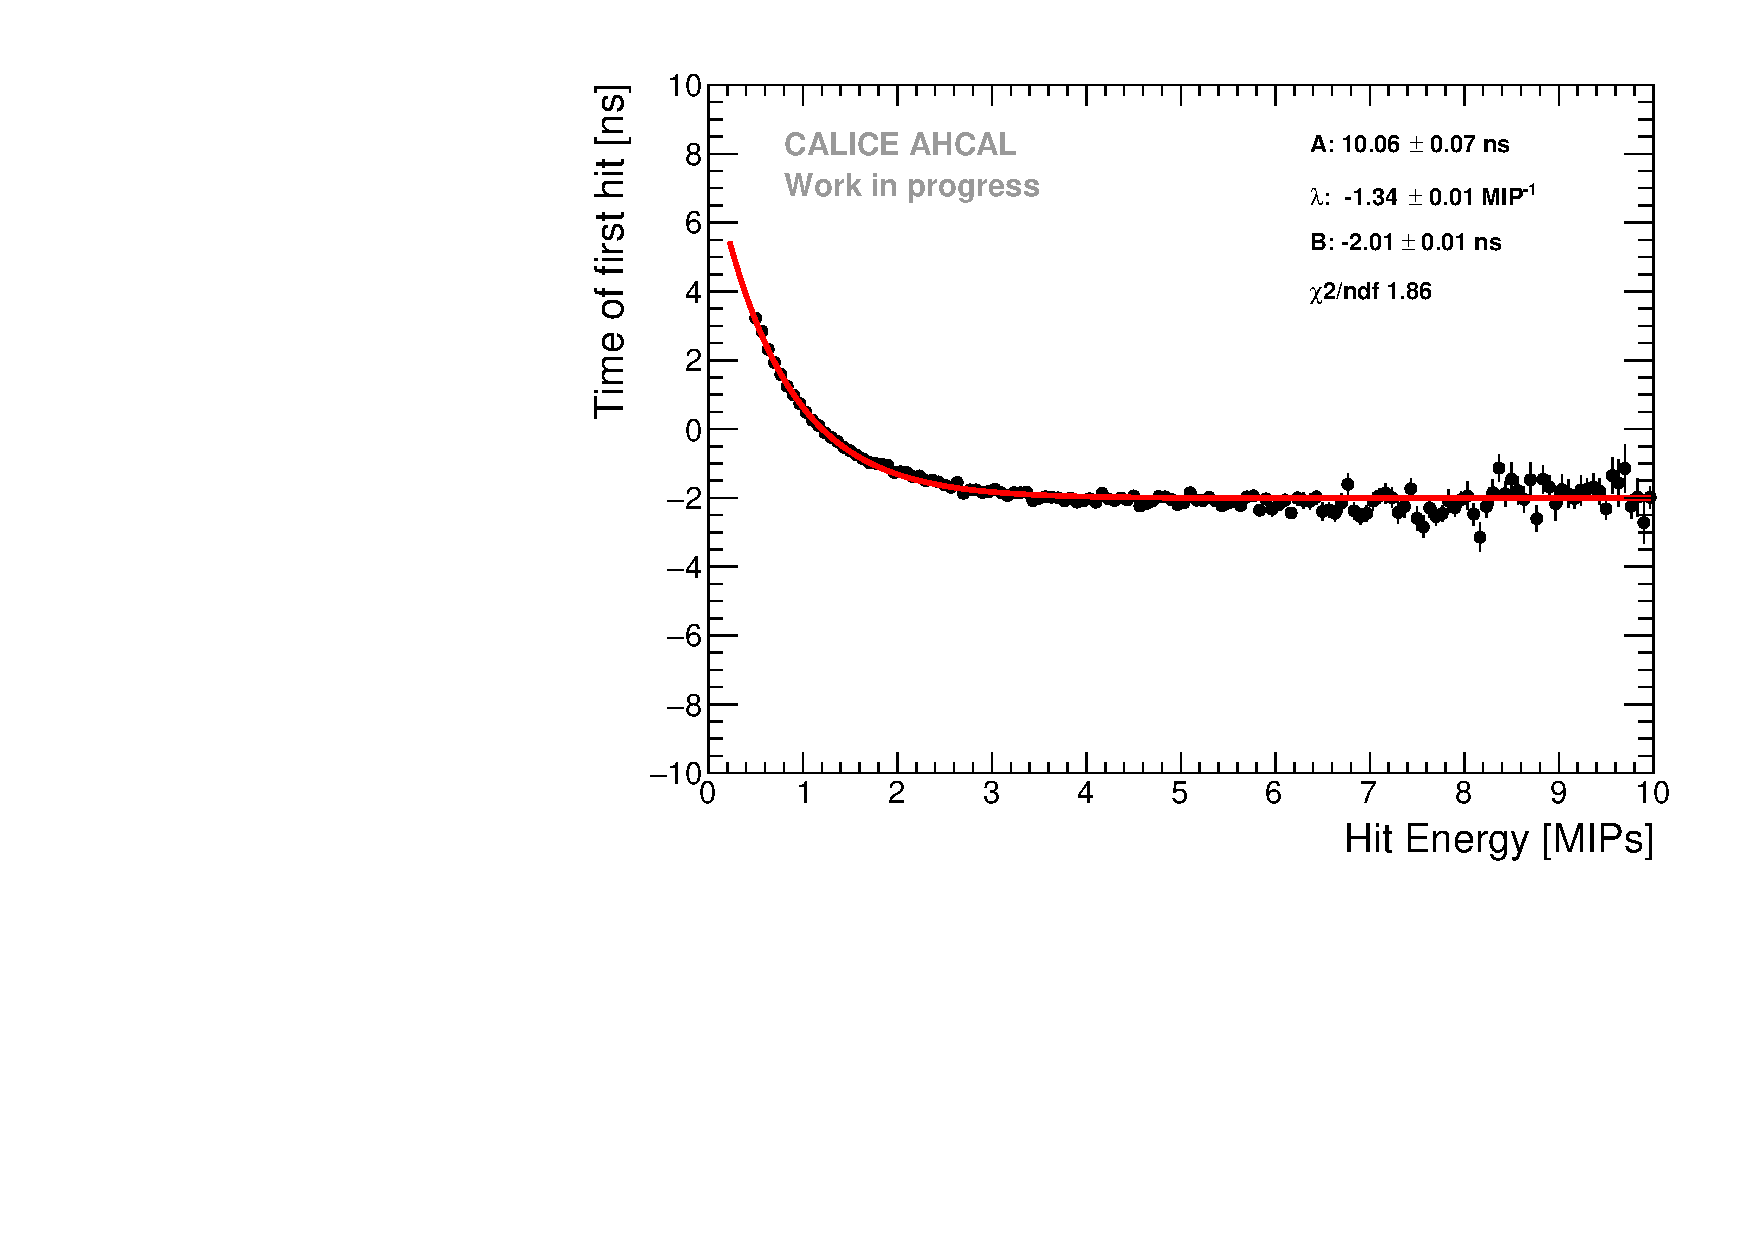
\includegraphics[width=0.5\textwidth]{fig/TimeWalkProfile.pdf}}\hfill
	\subfigure[Same profile after time-walk correction.\label{fig:time_walk_corr}] {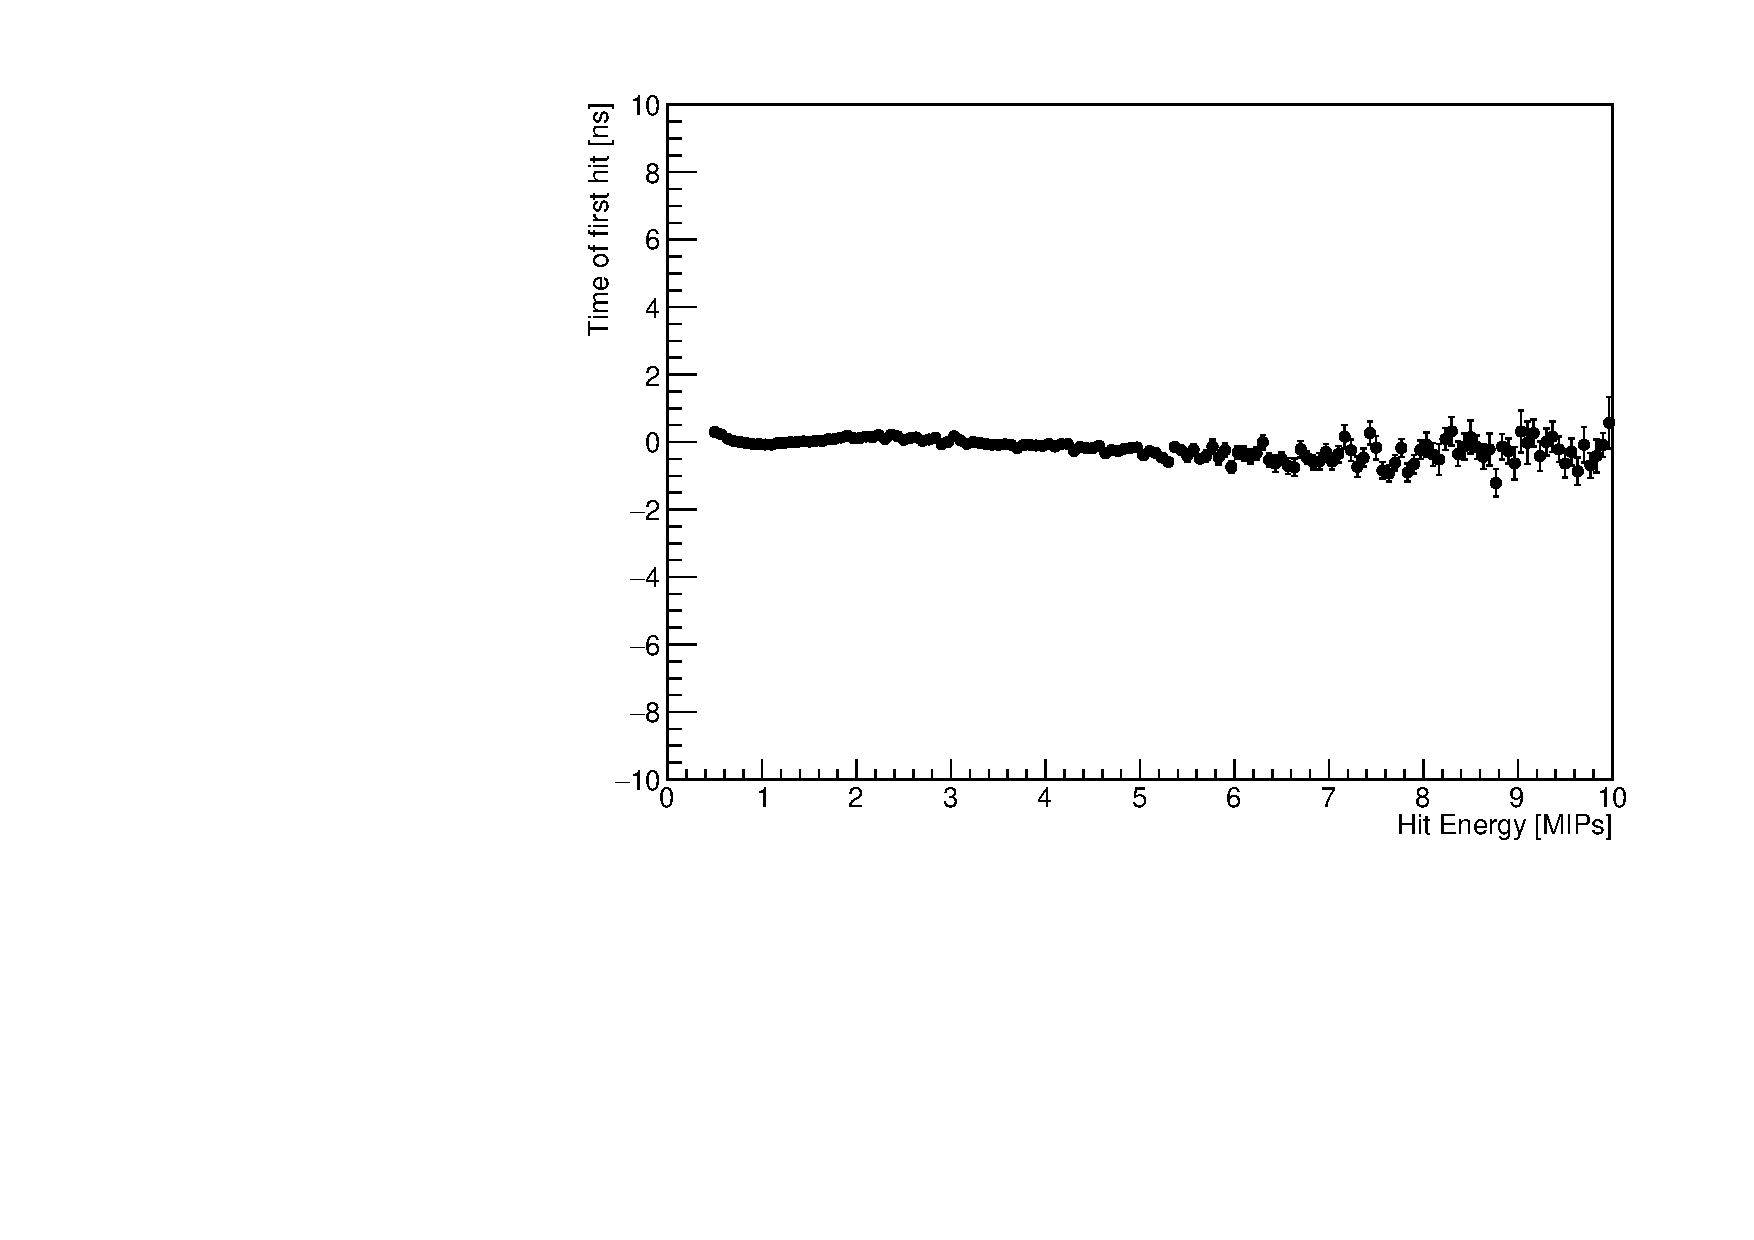
\includegraphics[width=0.5\textwidth]{fig/TimeWalkProfile_Correction.pdf}}
	\caption[]{\textbf{a}: Time-walk correction extracted from data. A = 10.38 $\pm$ 0.05, $\lambda$ = -1.21 $\pm$ 0.01, B = -2.24 $\pm$ 0.01. A difference up to 6 ns is seen between small and large amplitudes. \textbf{b}: Time-walk profile after correction showing a spread of less than 1 ns.}
\end{figure}
An improvement of $\sim$4\% can be achieved on the time resolution of the AHCAL (RMS 5.11 ns) as shown on figure \ref{fig:timing_reso_all_muons}. After all corrections, the distribution on figure \ref{fig:timing_muons} shows the time resolution obtained in the complete AHCAL excluding the layer 11 as well as the chip 157. The obtained time resolution is around 5 ns. The distribution is still asymmetric and it has been investigated, the asymmetry is certainly coming from the non-linearity of the TDC ramp of the trigger reference as no external time is available to correct for it. This is taken into account in the simulation by parametrizing the time distribution with a double Gaussian function.
\begin{figure}[htbp]
	\subfigure[Time resolution obtained for each AHCAL layers.\label{fig:timing_reso_all_muons}] {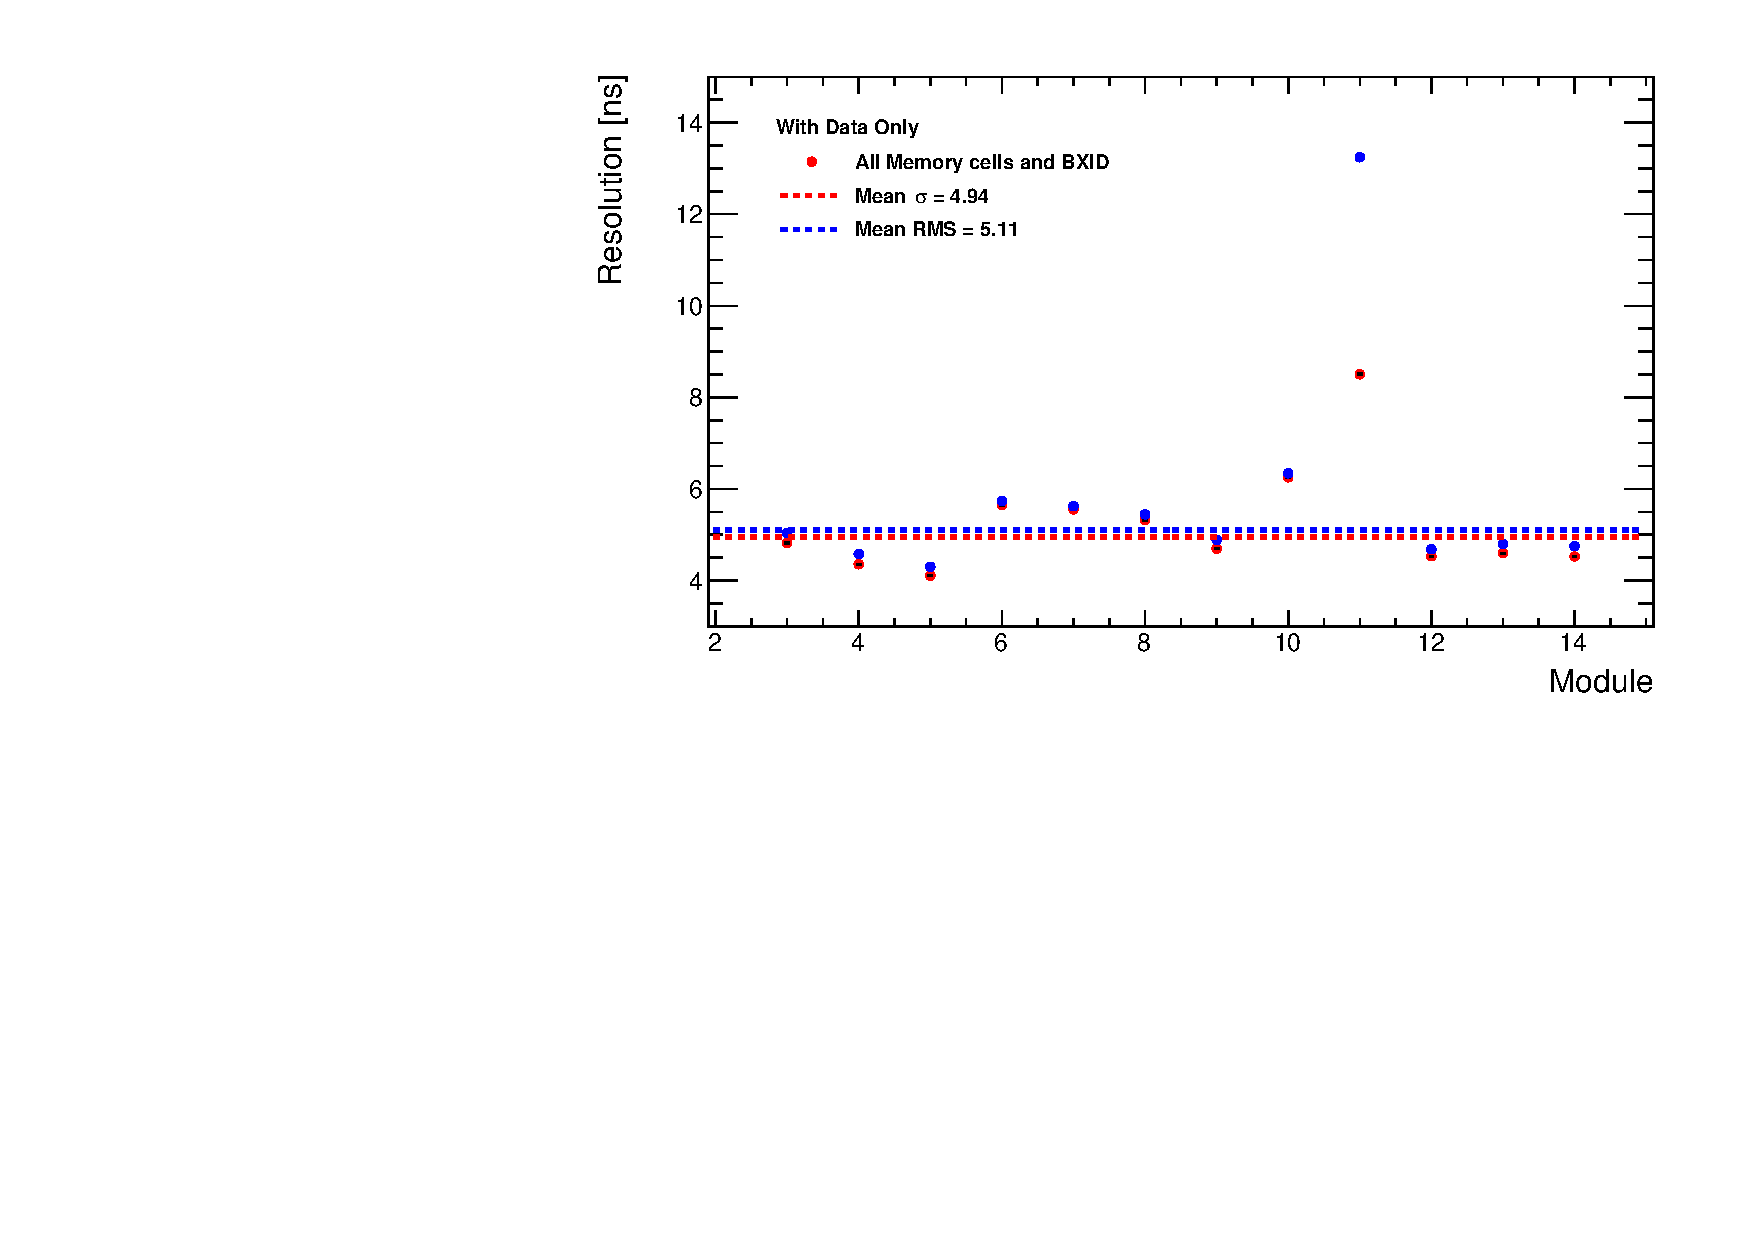
\includegraphics[width=0.5\textwidth]{fig/Muons_AllCorrections/ResolutionPerModule_All.pdf}}\hfill
	\subfigure[Time of the first hit distribution of the AHCAL after all corrections.\label{fig:timing_muons}] {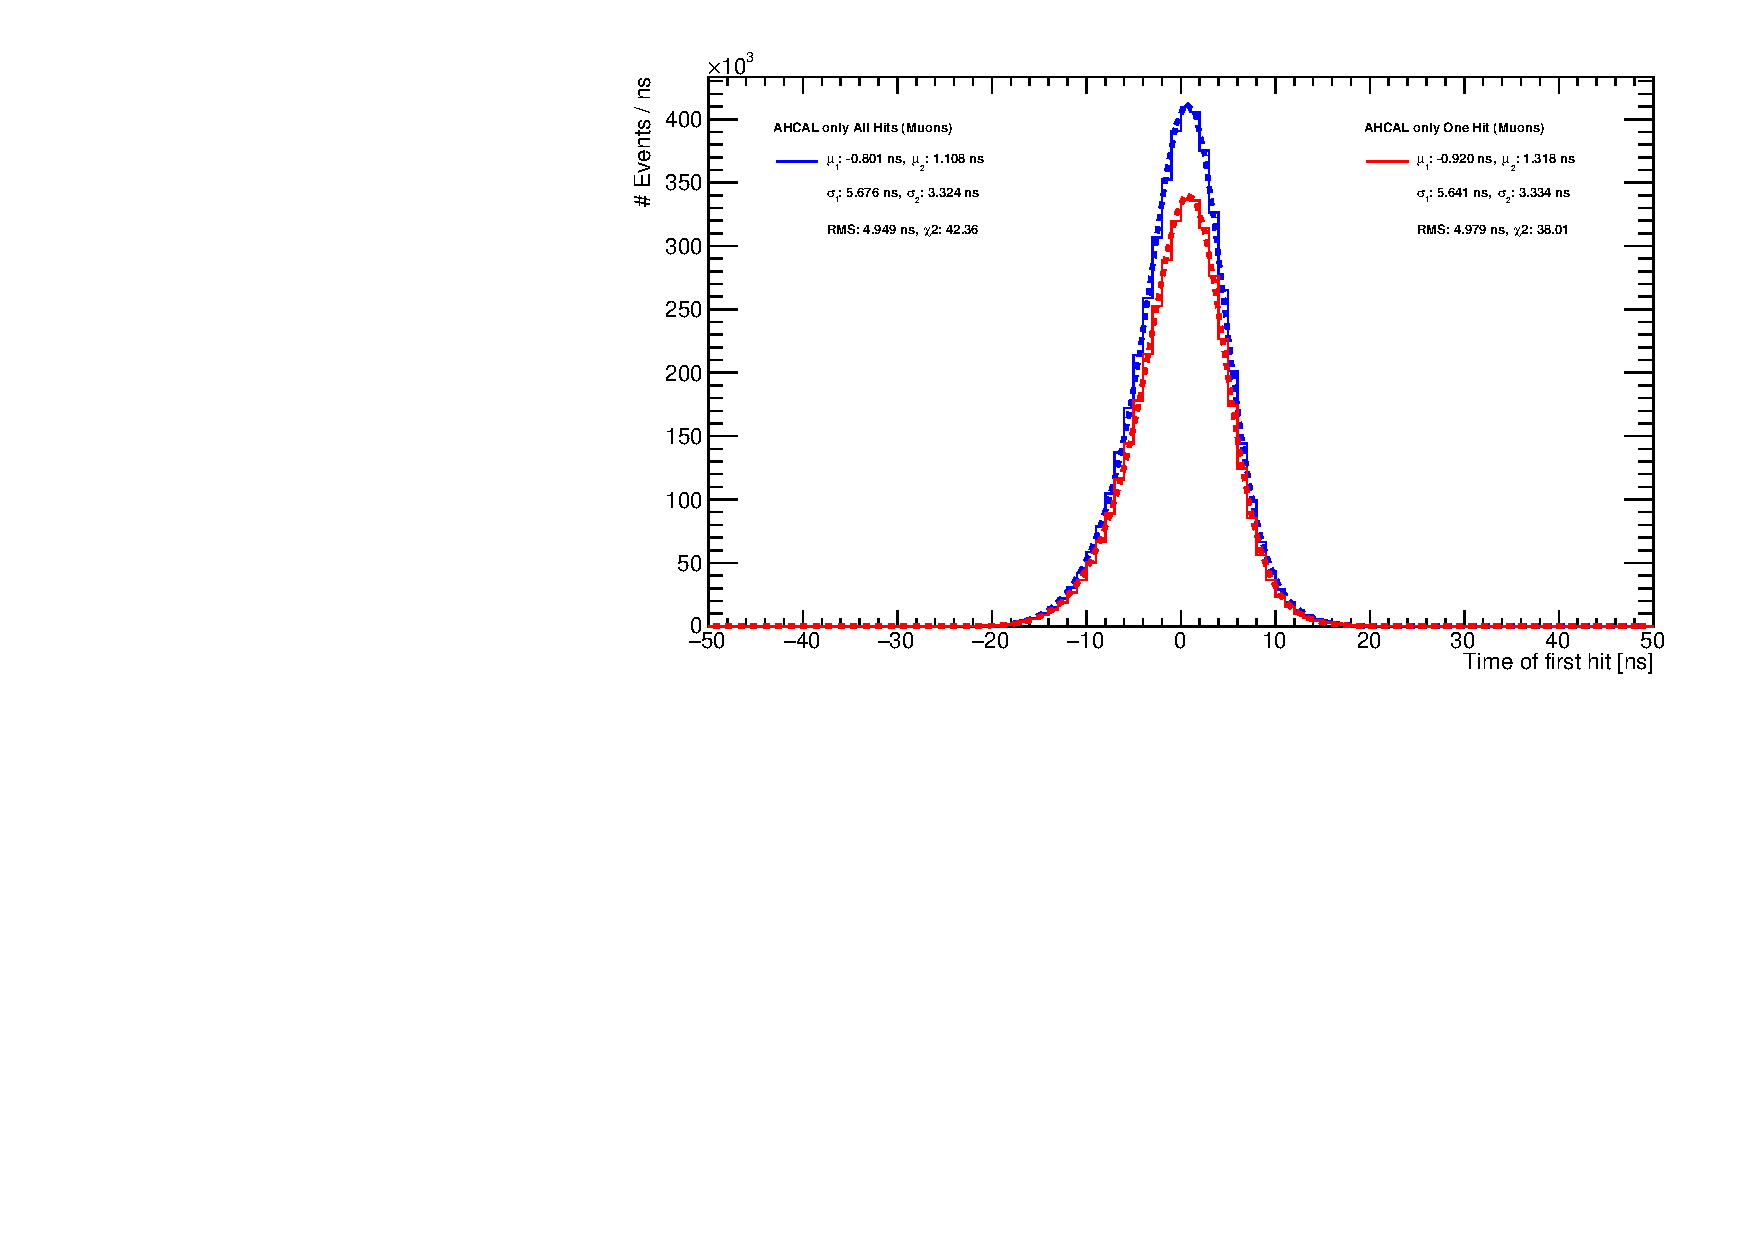
\includegraphics[width=0.5\textwidth]{fig/Timing_Muons.pdf}}
	\caption[]{\textbf{a}: Time resolution obtained for each layer in the AHCAL. Mean RMS = 5.11 ns \textbf{b}: The red distribution considers only track with single hit per layer. The blue distribution take into account all the hits from muon tracks. RMS$_{\text{One Hit}}$ = 4.98 ns, RMS$_{\text{All Hits}}$ = 4.95 ns.}
\end{figure}

\subsection{Electron Selection}
\label{subsec:elec_sel}

To perform comparisons on electron, a sample of electron events is selected from the data runs. A simple selection is performed in order to have mostly contained showers in the AHCAL. The selection requires at least 50 hits in the AHCAL, a fiducial cut of $80\times80\times360$ mm$^3$ on the center of gravity of the shower in x, y and z is made and less than 0.1\% of the energy sum should be contained in the last two layers.

\subsection{Cross-check of the calibration with electrons}
\label{subsec:validation}

In order to validate the calibration, an electron sample is taken. Electromagnetic showers are quasi-instantaneous and perfect to cross-check the time calibration procedure. The selection applied to the data sample is described in subsection \ref{subsec:elec_sel}. The same calibration constants and correction constants are applied to the data except that an additional offset from the trigger signal has to be corrected for. The additional offset is expected to be small as the trigger configuration is very similar to the one for muons. The offset is in the order of 10 ns which is consistent with the changes in trigger configuration. The time of the first hit distribution is shown in figure \ref{fig:Timing_electrons}.
\begin{figure}[htbp]
\begin{center}
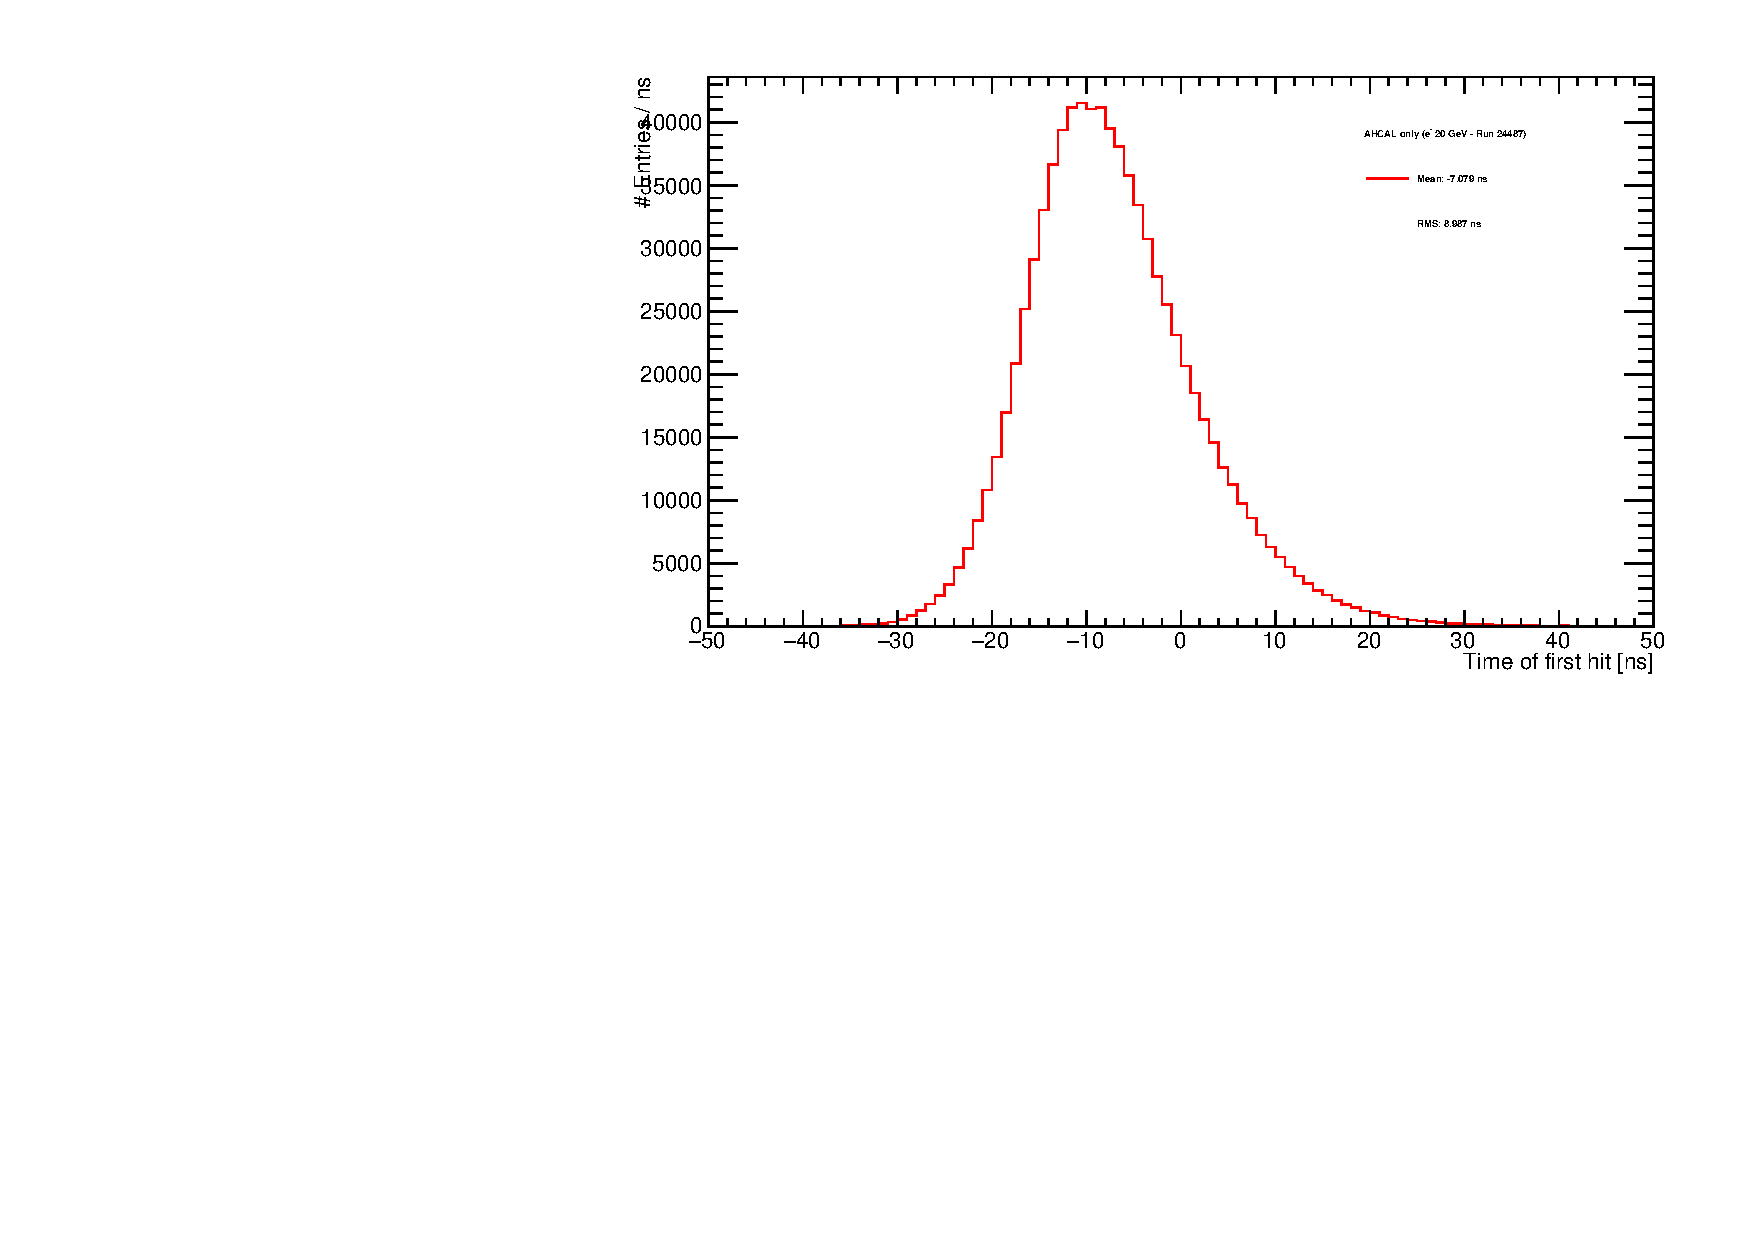
\includegraphics[width=0.6\textwidth]{fig/Electrons_MuonCalib/Timing_AllLayers.pdf}
\caption{Time of the first hit distribution for 20 GeV electrons, Max = 10.05 ns, RMS = 8.94 ns.}
\label{fig:Timing_electrons}
\end{center}
\end{figure}
The time distribution presents a large tail to the right and moreover is much wider than for muons. This gives a hint that an effect is present in electron data but not in muon data. The difference seen could be related to the fact that in electromagnetic showers, the number of hits is much higher as well as the energy deposited in a single cell can be over hundreds MIP. Moreover, the time distribution contains all layer of the AHCAL except layer 11, 4 and 5 and chip 157. The layer 4 and 5 time distributions have been investigated and they present a long tail to the right due to the effect presented in subsection \ref{subsec:ped_shift} as theses layers are located in the expected shower maximum for 20 GeV electrons.

\subsection{Influence of the number of triggered channels}
\label{subsec:ped_shift}
%TO BE SORTED!!
Pedestal shift for energy measurement is not a new feature of the SPIROC2b chip and is still intensively investigated \cite{OskarMaster}. The effect comes most likely from the fact that a ground shift occurs in the chip when a saturated signal (high current) is present in a several channels. It may as well induce a shift of the trigger threshold and thus can have an impact on the time of the hit. This effect can be investigated by looking at the time of the first hit as a function of the number of triggered channels over 0.5 MIP. This has been done as shown in figure \ref{fig:nhits_profile}.
\begin{figure}[htbp]
	\subfigure[Time of the first hit function of the number of triggered channels in a chip.\label{fig:nhits_profile}] {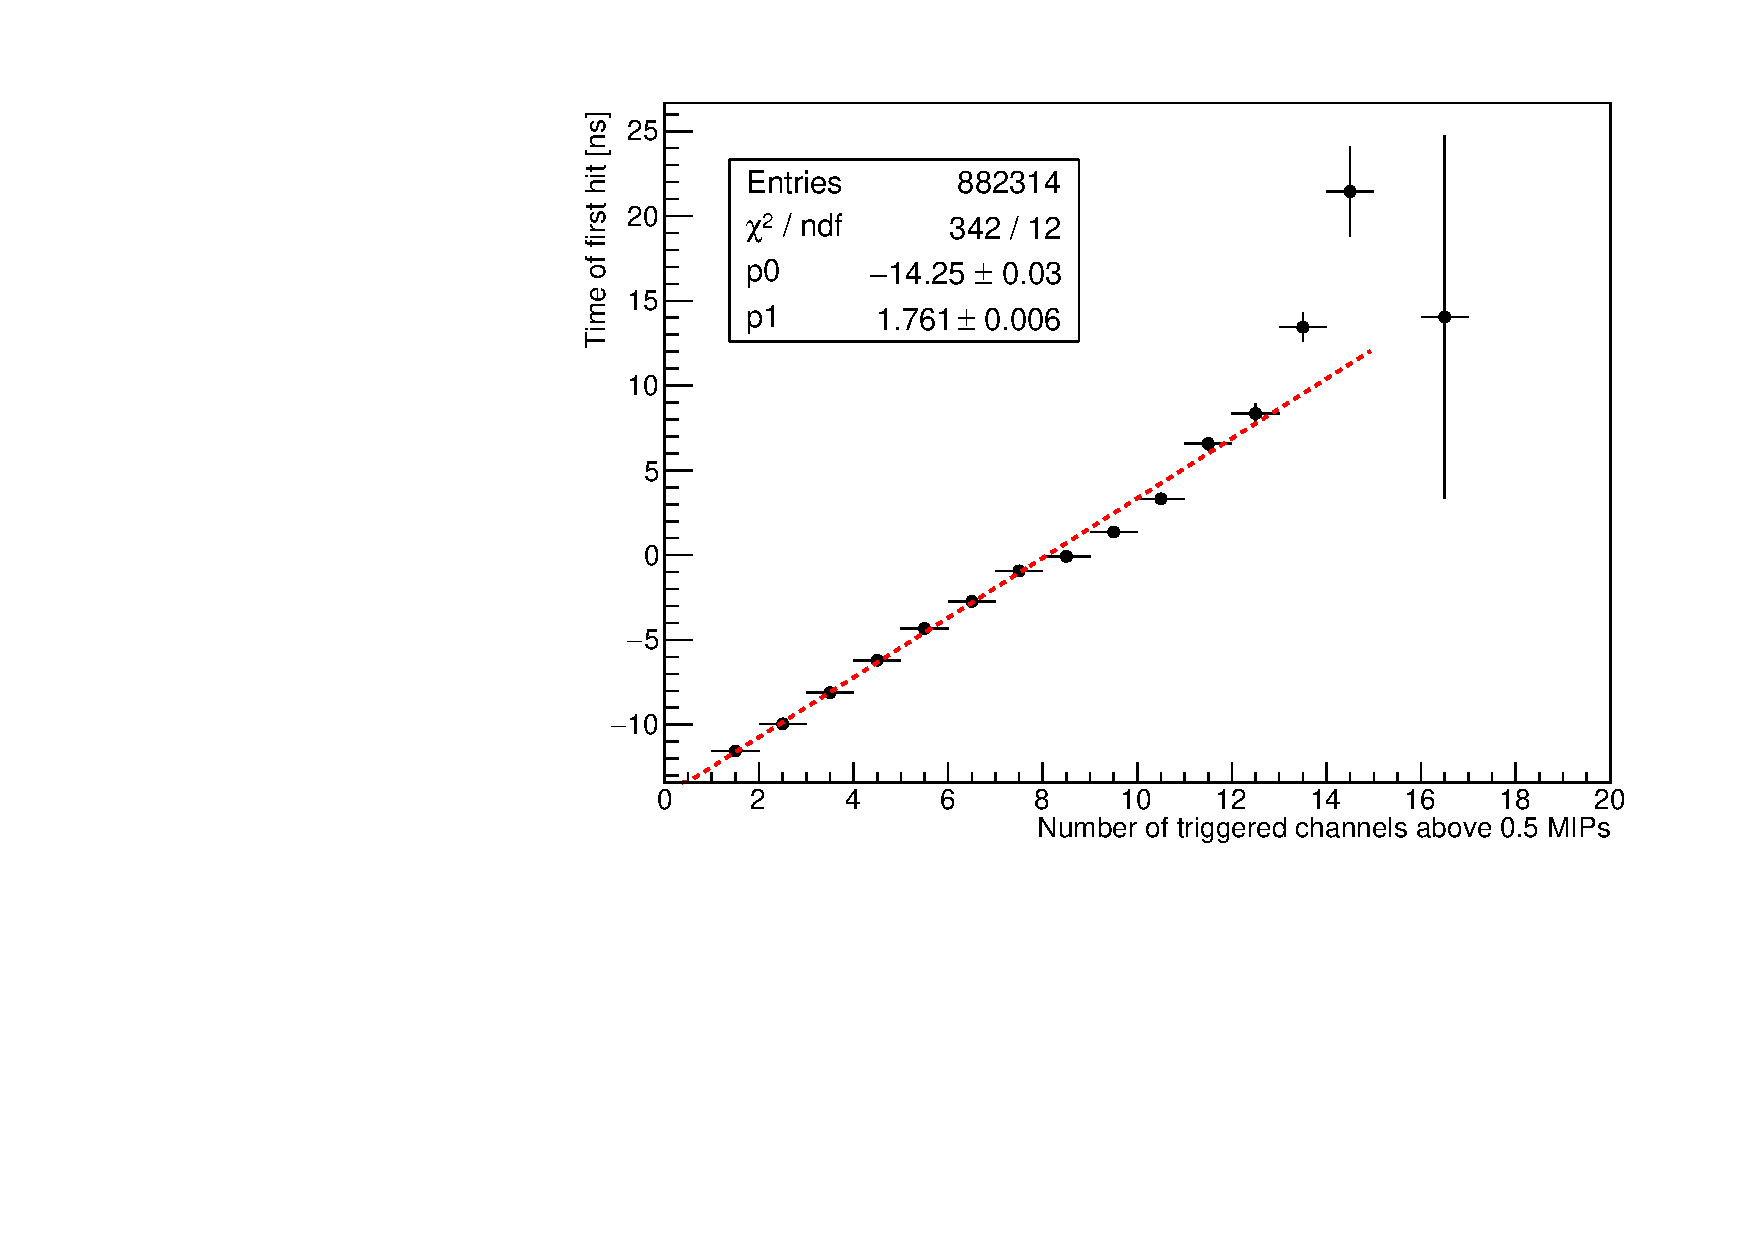
\includegraphics[width=0.5\textwidth]{fig/NumberHits_Dependance.pdf}}\hfill
	\subfigure[RMS of the time of first hit function of the number of triggered channels.\label{fig:RMS_nHits}] {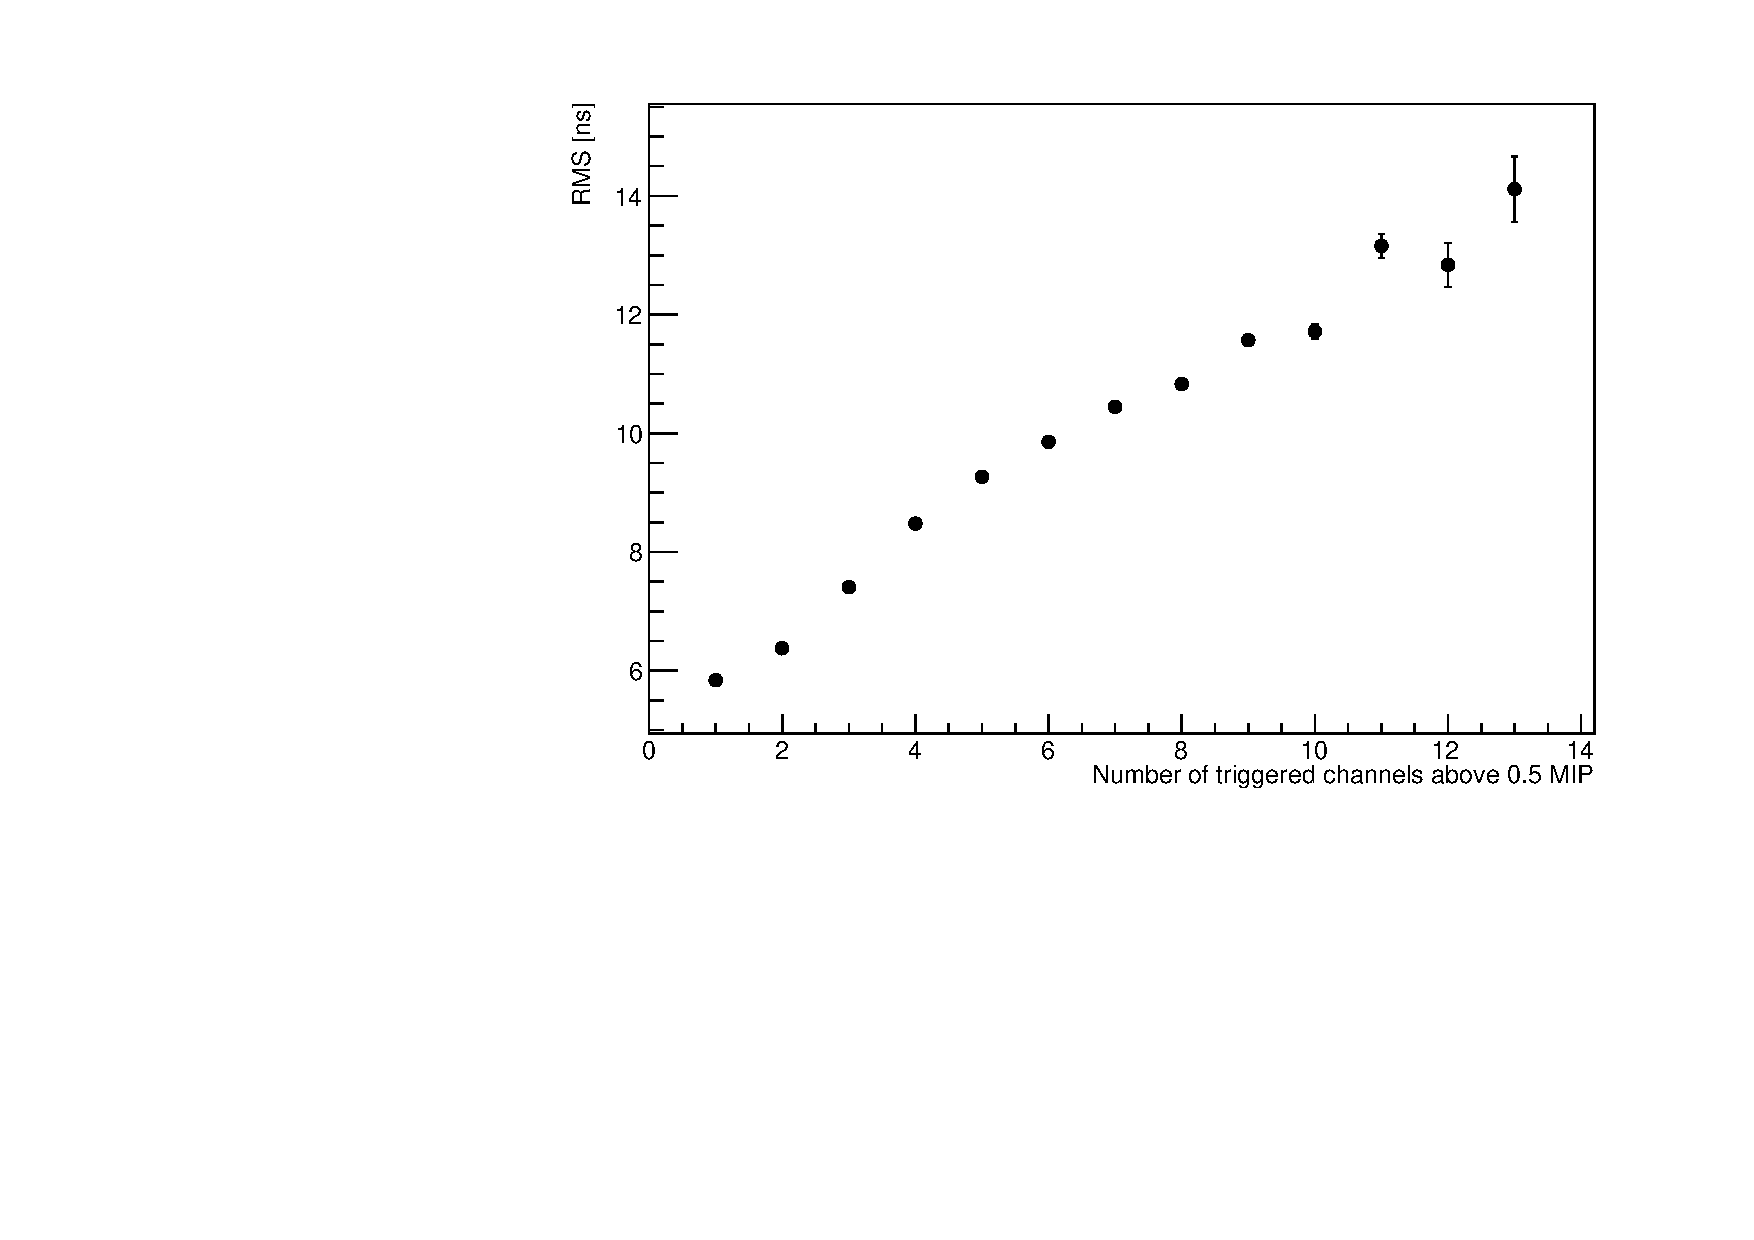
\includegraphics[width=0.5\textwidth]{fig/ParametrisationPedestalShift.pdf}}
	\caption[]{\textbf{a}: The fit region is between 1 and 15 hits. A linear dependence is clearly visible. \textbf{b}: The RMS of the time distribution can increase up to 15 ns for a high number of triggered channels.}
\end{figure}
The effect can have a drastic effect on the time resolution of the AHCAL, a correction up to 15 ns can be necessary to the data for a high number of trigger. The cause of this effect is thought to be due to an element in the chip (a delay box) that get unstable with the number of triggered channels and that is responsible for the hold of the TDC value in the chip. The hold is delayed thus sampling a higher TDC value than the one expected. Once the parameters for the correction have been determined with a linear fit, it is applied to the electron data sample and the distribution of the time of the first is again shown in figure \ref{fig:timing_electrons_corr}.
\begin{figure}[htbp]
	\subfigure[Time of the first hit distribution for 20 GeV electrons after correction.\label{fig:timing_electrons_corr}] {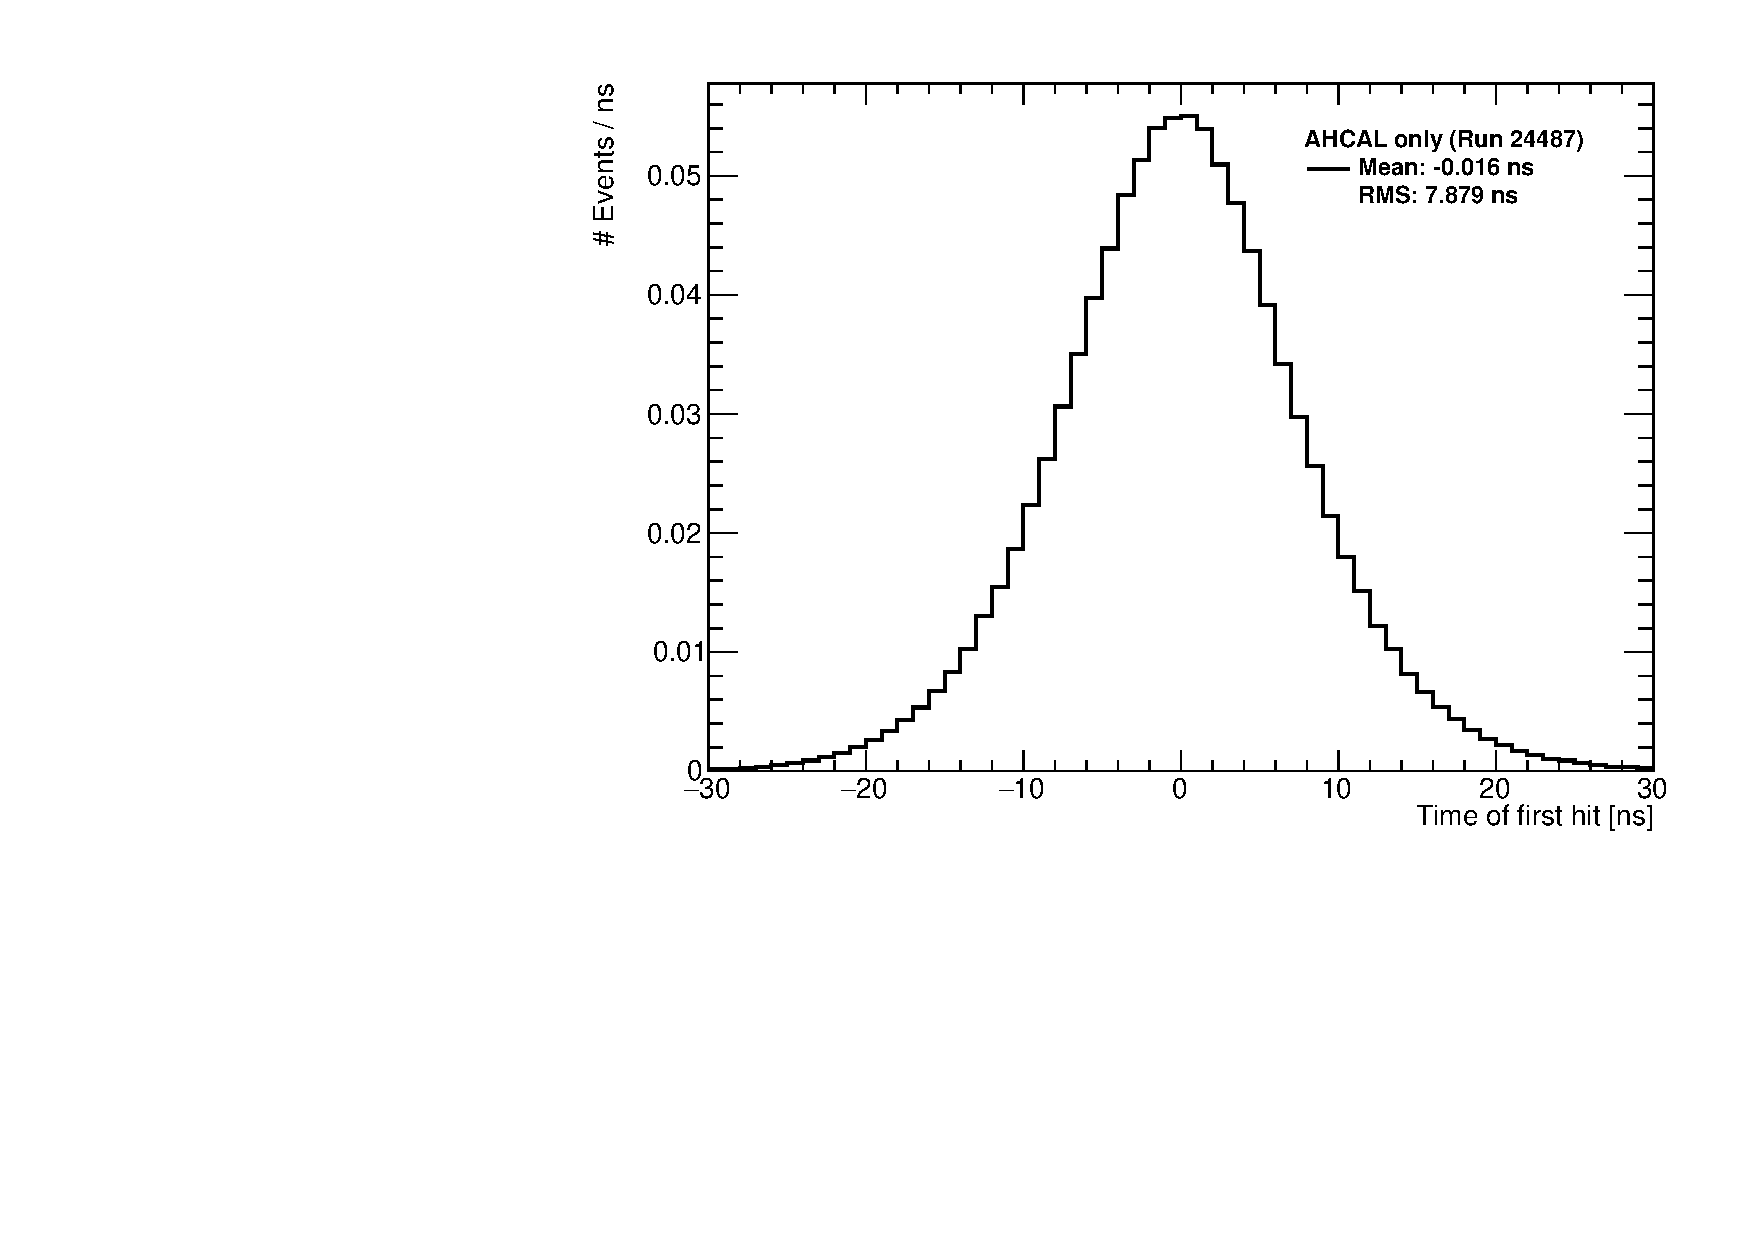
\includegraphics[width=0.5\textwidth]{fig/Electrons_Full/Timing_AllLayers.pdf}}\hfill
	\subfigure[Comparison with the muon time of first hit distribution.\label{fig:timing_electron_muon_comp}] {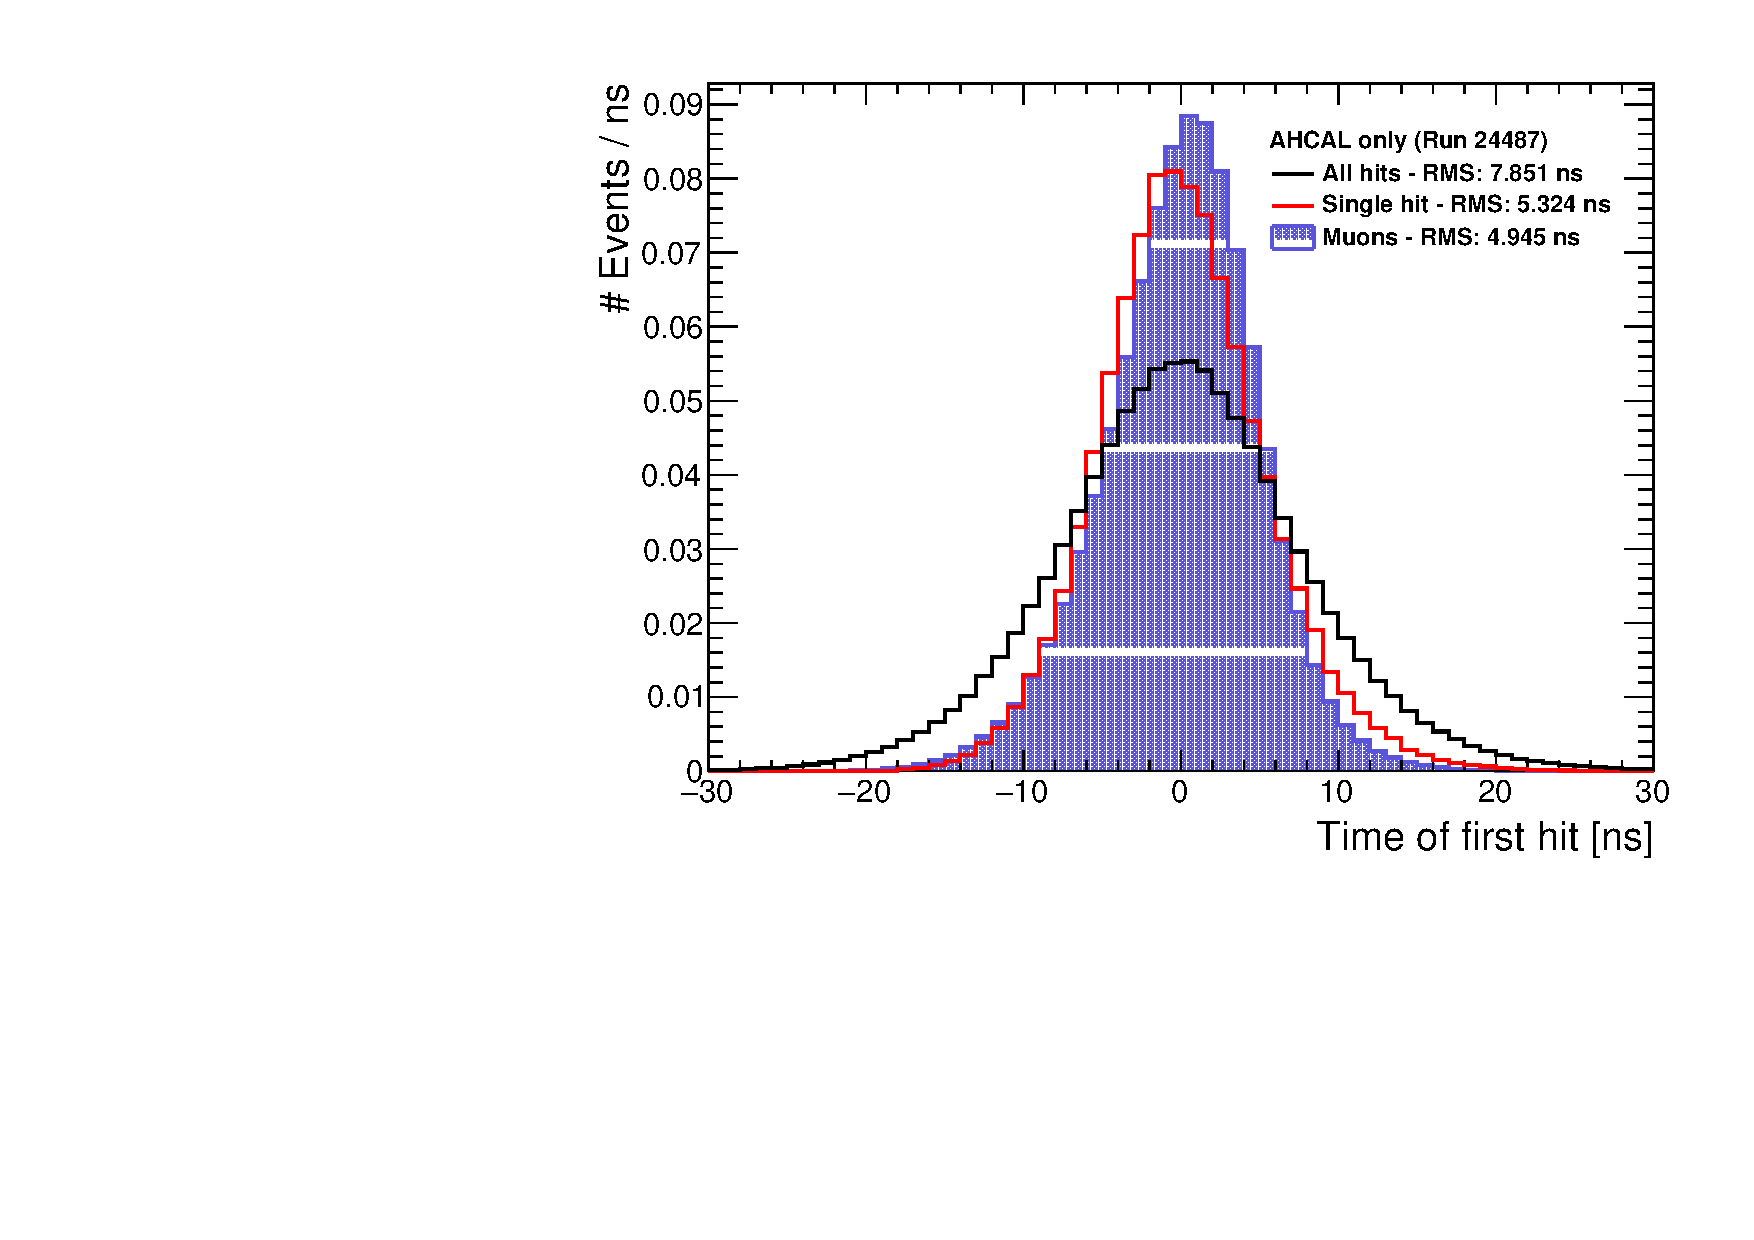
\includegraphics[width=0.5\textwidth]{fig/Electrons_Full/ComparisonAll_ElectronsSingleHit.pdf}}
	\caption[]{\textbf{a}: Time of the first hit distribution for 20 GeV electrons after number of triggered channel correction, $\mu$ = -0.01 ns, RMS = 7.85 ns. \textbf{b}: Comparison of the electron data sample, as expected the time distribution is very similar to the muon one if only events with single hits in a chip are taken.}
\end{figure}
As expected the correction improves the RMS of the distribution ($\sim$3.3\%) as well as the distribution appears more gaussian-like. However, there is still a discrepancy with the time resolution from muons ($\sim$36.9\% difference). This might indicates that the number of hits correction is only a mean correction of the effect thus it does not perform perfectly. In order for the simulation to match the data, the increase of the width of the distribution has to be parametrised from the data. More details can be read in the appendix \ref{appendix:ped_shift}. A comparison with the muon data has been done in order to check the calibration as seen on figure \ref{fig:timing_electron_muon_comp}. As expected if only single hits in a chip are taken, the time resolution obtained is very similar to the time resolution observed in muons ($\sim$7.1\% difference).

\subsection{Comparison with Simulation}

The next step is to compare data with simulation and validate the simulation with electrons. The timing resolution is extracted from muon data runs for each layer by fitting a double Gaussian in the range [-50 ns, 50 ns] and is used to smear the timing of simulated hits. The table \ref{table:time_res_sim} sums up the resolution used.
\begin{table}[htbp]
\centering
  \begin{tabular}{@{} ccccc @{}}
    \hline
    Layer & $\mu_{1}$ & $\sigma_{1}$ & $\mu_{2}$ & $\sigma_{2}$ \\ 
    \hline
    3 & -1.54 & 5.74 & 1.52 & 3.62 \\
    4 & -0.96 & 5.46 & 0.96 & 3.15 \\
    5 & -0.44 & 5.05 & 0.53 & 2.92 \\
    6 & -0.74 & 6.03 & 2.70 & 3.12\footnotemark[1] \\
    7 & -0.54 & 5.88 & 2.34 & 3.17 \\
    8 & -0.51 & 5.92 & 1.26 & 3.40 \\
    \hline
  \end{tabular}
  \hspace{2ex}
  \begin{tabular}{@{} ccccc @{}}
    \hline
    Layer & $\mu_{1}$ & $\sigma_{1}$ & $\mu_{2}$ & $\sigma_{2}$ \\ 
    \hline
    9 & -0.31 & 5.97 & 0.25 & 3.62 \\
    10 & -0.62 & 5.97 & 4.58 & 6.93 \\
    11 & -4.40 & 6.18 & 8.82 & 19.12\footnotemark[1] \\
    12 & -0.94 & 5.26 & 1.39 & 3.16 \\
    13 & -1.18 & 5.49 & 1.42 & 3.27 \\
    14 & -1.19 & 5.55 & 1.25 & 3.27 \\
	\hline
  \end{tabular}
  \caption{Timing resolution extracted with a double Gaussian fit from muon data used for simulation.}
  \label{table:time_res_sim}
\end{table}
\footnotetext{The chips on layer 11 have a noisy problem leading to a right tail in the distribution and thus are excluded. The chip 157 on layer 6 is also excluded (broken chip).} 
The comparison for muons is shown on figure \ref{fig:sim_data_muon}. The number of hits correction is not applied as it is supposed to be negligible for muons. Generally 1 or 2 channels can be triggered in the same chip at maximum thus limiting effect.
\begin{figure}[htbp]
	\subfigure[Time of first hit for data and simulation between -50 and 50 ns.\label{fig:muon_sim_data_1}] {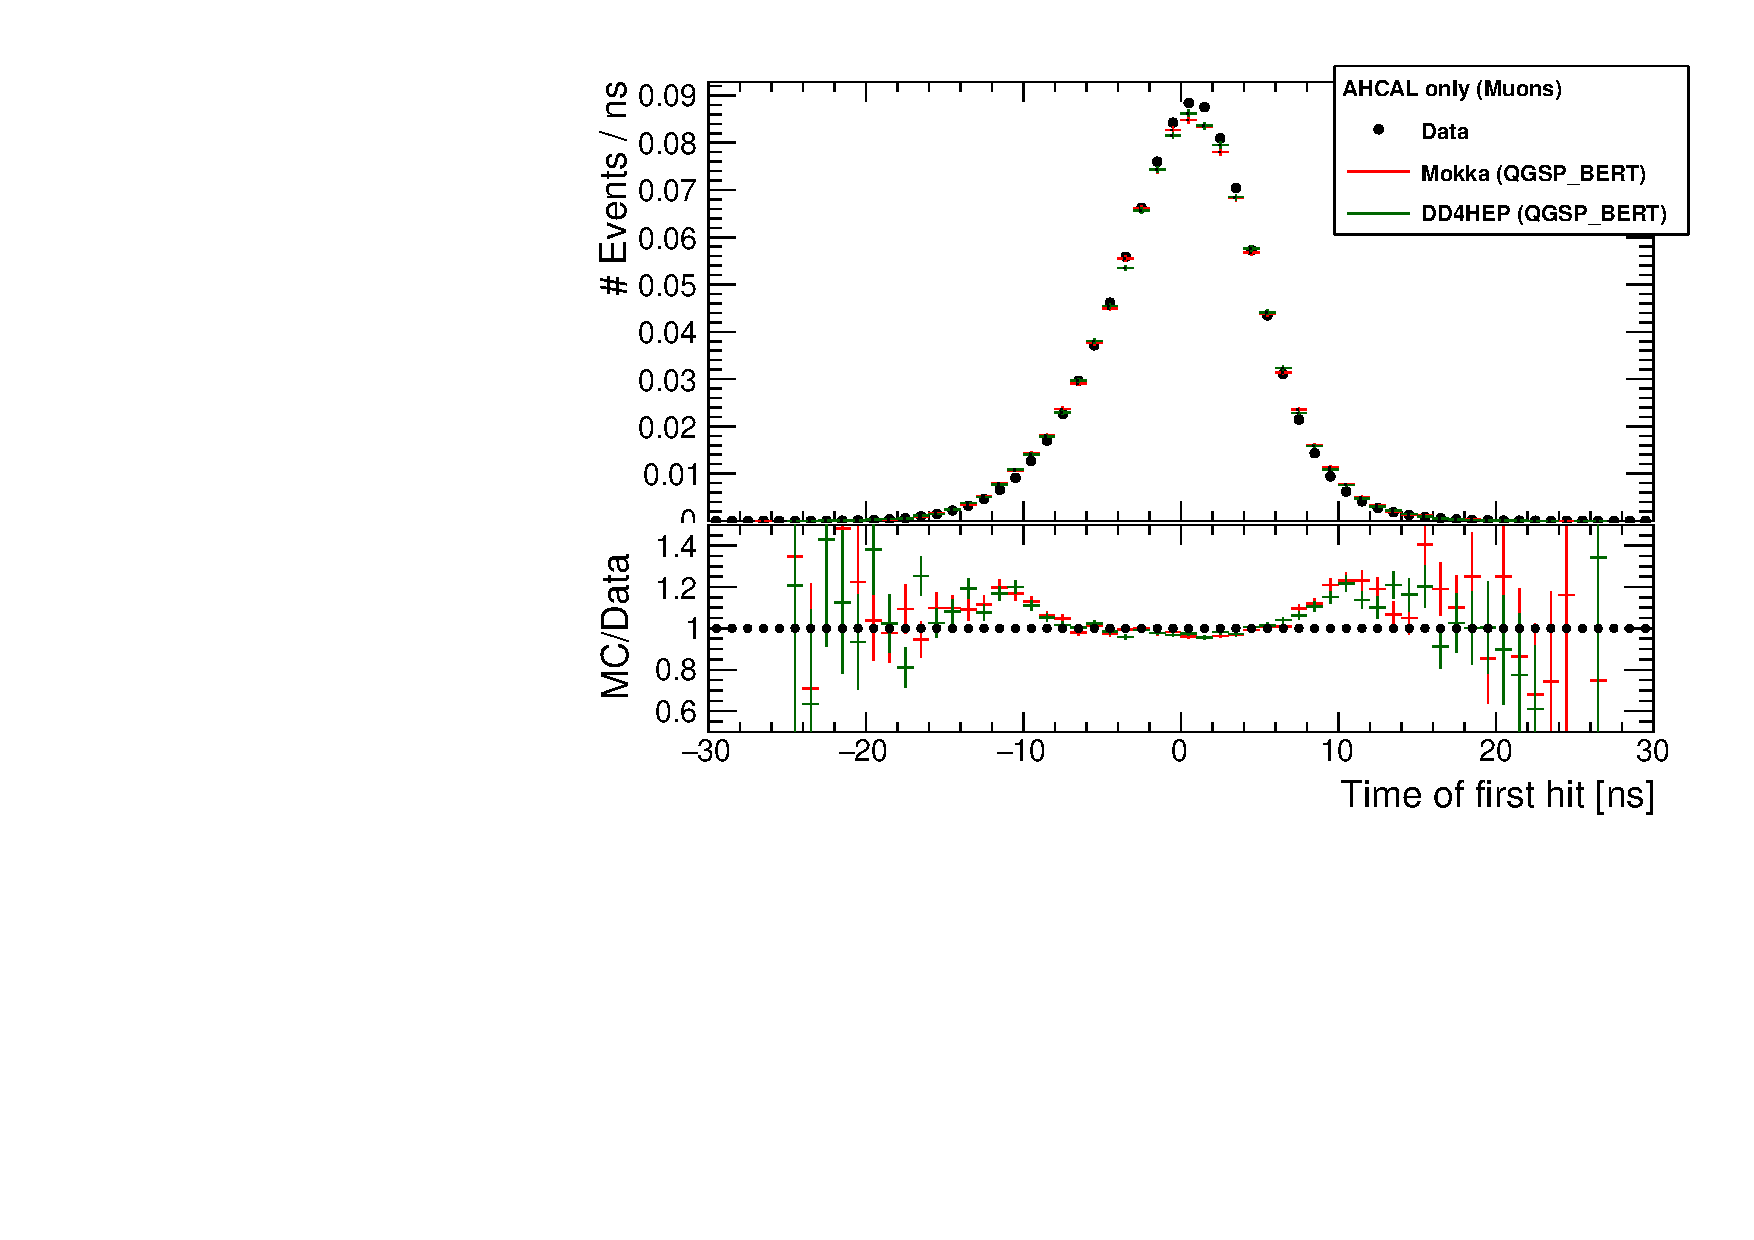
\includegraphics[width=0.5\textwidth]{fig/Simulation_Muons/Comparison_SimData_Muons.pdf}}\hfill
	\subfigure[Time of first hit for data and simulation zoomed between 1 and 200 ns.\label{fig:muon_sim_data_2}] {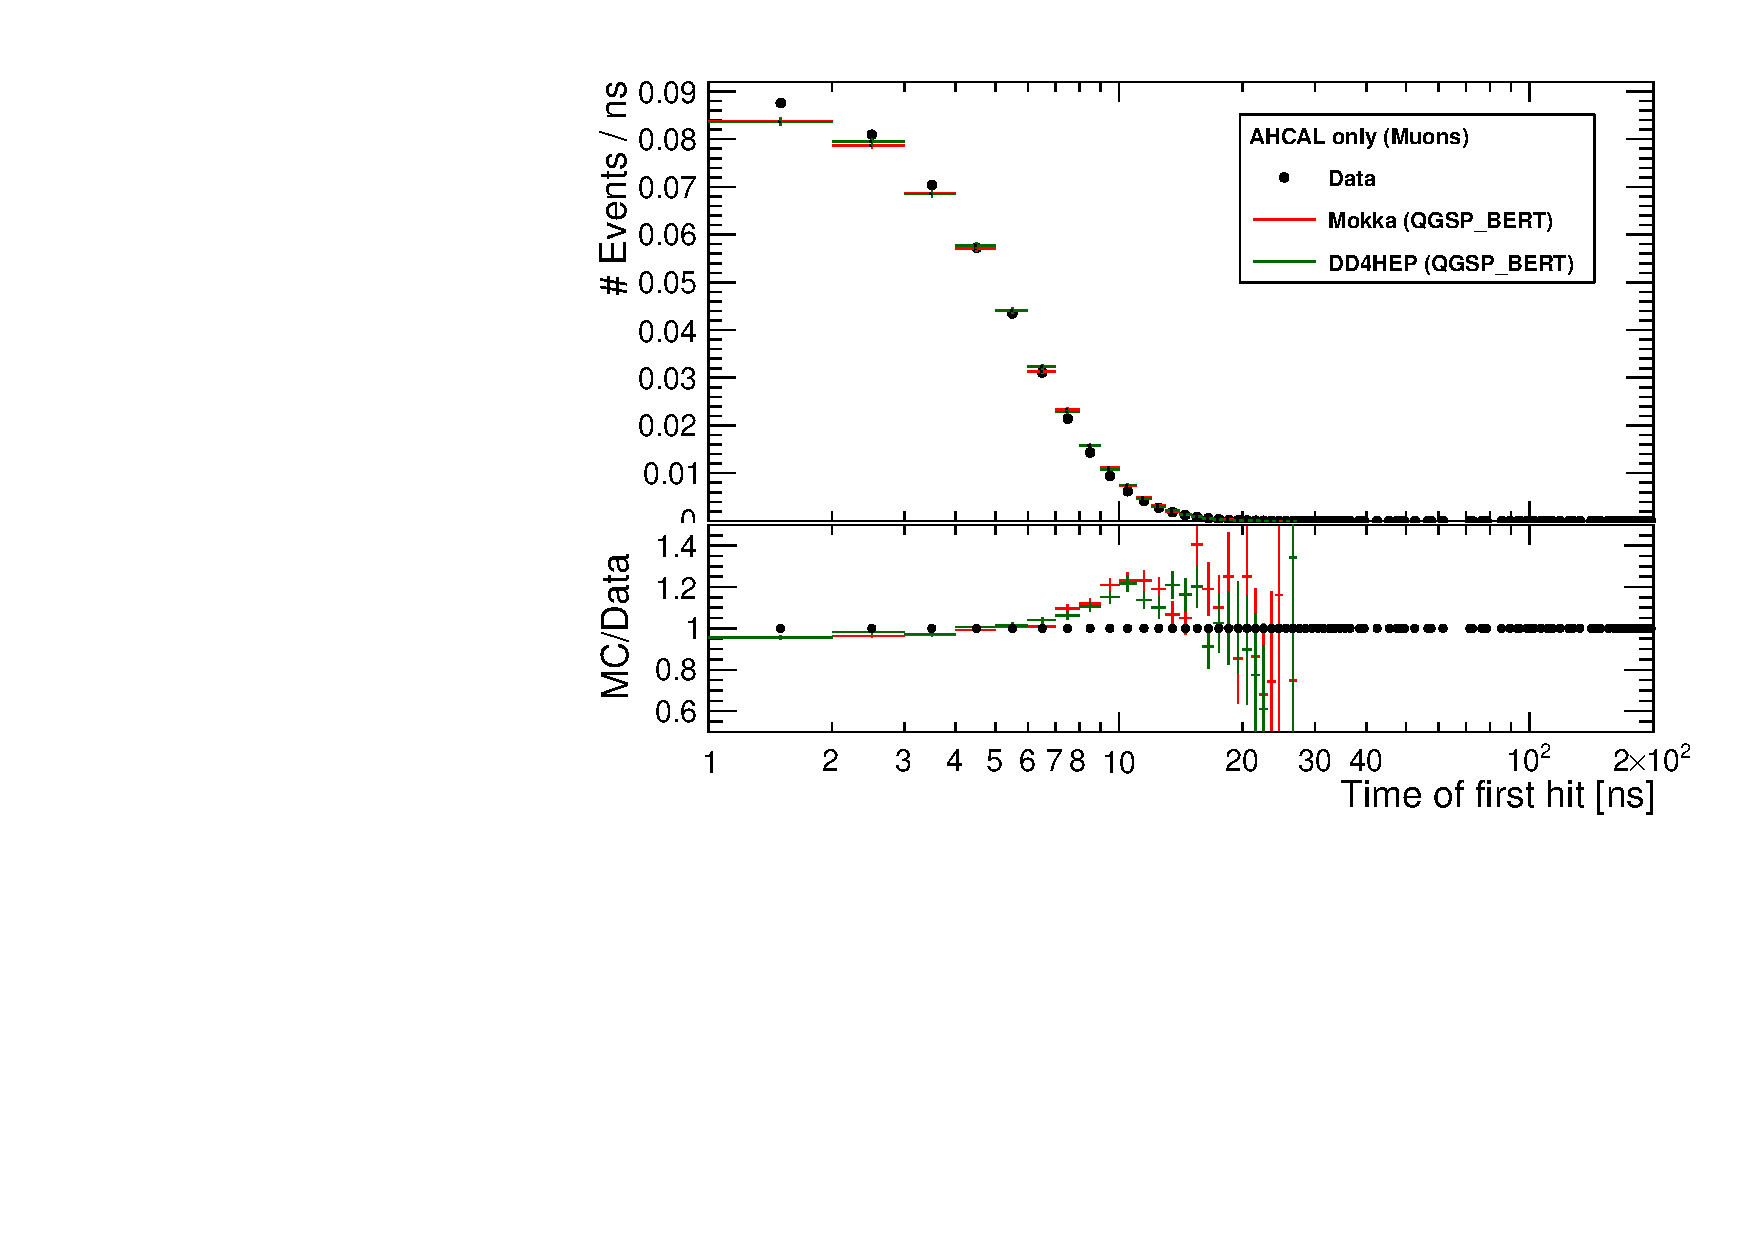
\includegraphics[width=0.5\textwidth]{fig/Simulation_Muons/Comparison_SimData_Muons_zoom.pdf}}
	\caption[]{\textbf{a}: The simulation agrees well with the data in the region -10 to 10 ns (up to 20\% deviation). \textbf{b}: Zoom in the region 1 to 200 ns, the agreement is worse between 10-20 ns, this may be from an incomplete description of the asymmetry seen in the data.}
	\label{fig:sim_data_muon}
\end{figure}
The comparison shows that in the range [-10, 10] ns, the difference between data and simulation is around 20\% maximum. Under -10 ns, the simulation is much more in disagreement due to the asymmetric shape in data that is not well reproduced in simulation. On the right side of the time distribution, between 10 and 20 ns, the agreement between data and Monte-Carlo worsens. This is certainly because of the tail present in data that might be not well reproduced in Monte-Carlo. Theses distributions show that the simulation performs well in the first tens of nanoseconds but that more work needs to be invested in the reproduction of the data up to 200 ns which is important for hadronic showers.\\
In the next step, a comparison with electron data is necessary to validate the simulation. The time resolution used for each layer is the same shown in table \ref{table:time_res_sim}. In addition, a parametrisation of the increase of the width of the time distribution function of the number of hits above 0.5 MIPs is added as describe in appendix \ref{appendix:ped_shift}. The figures \ref{fig:sim_data_elec} shows this comparison.
\begin{figure}[htbp]
	\subfigure[Time of first hit for data and simulation between -30 and 30 ns.\label{fig:elec_sim_data_1}] {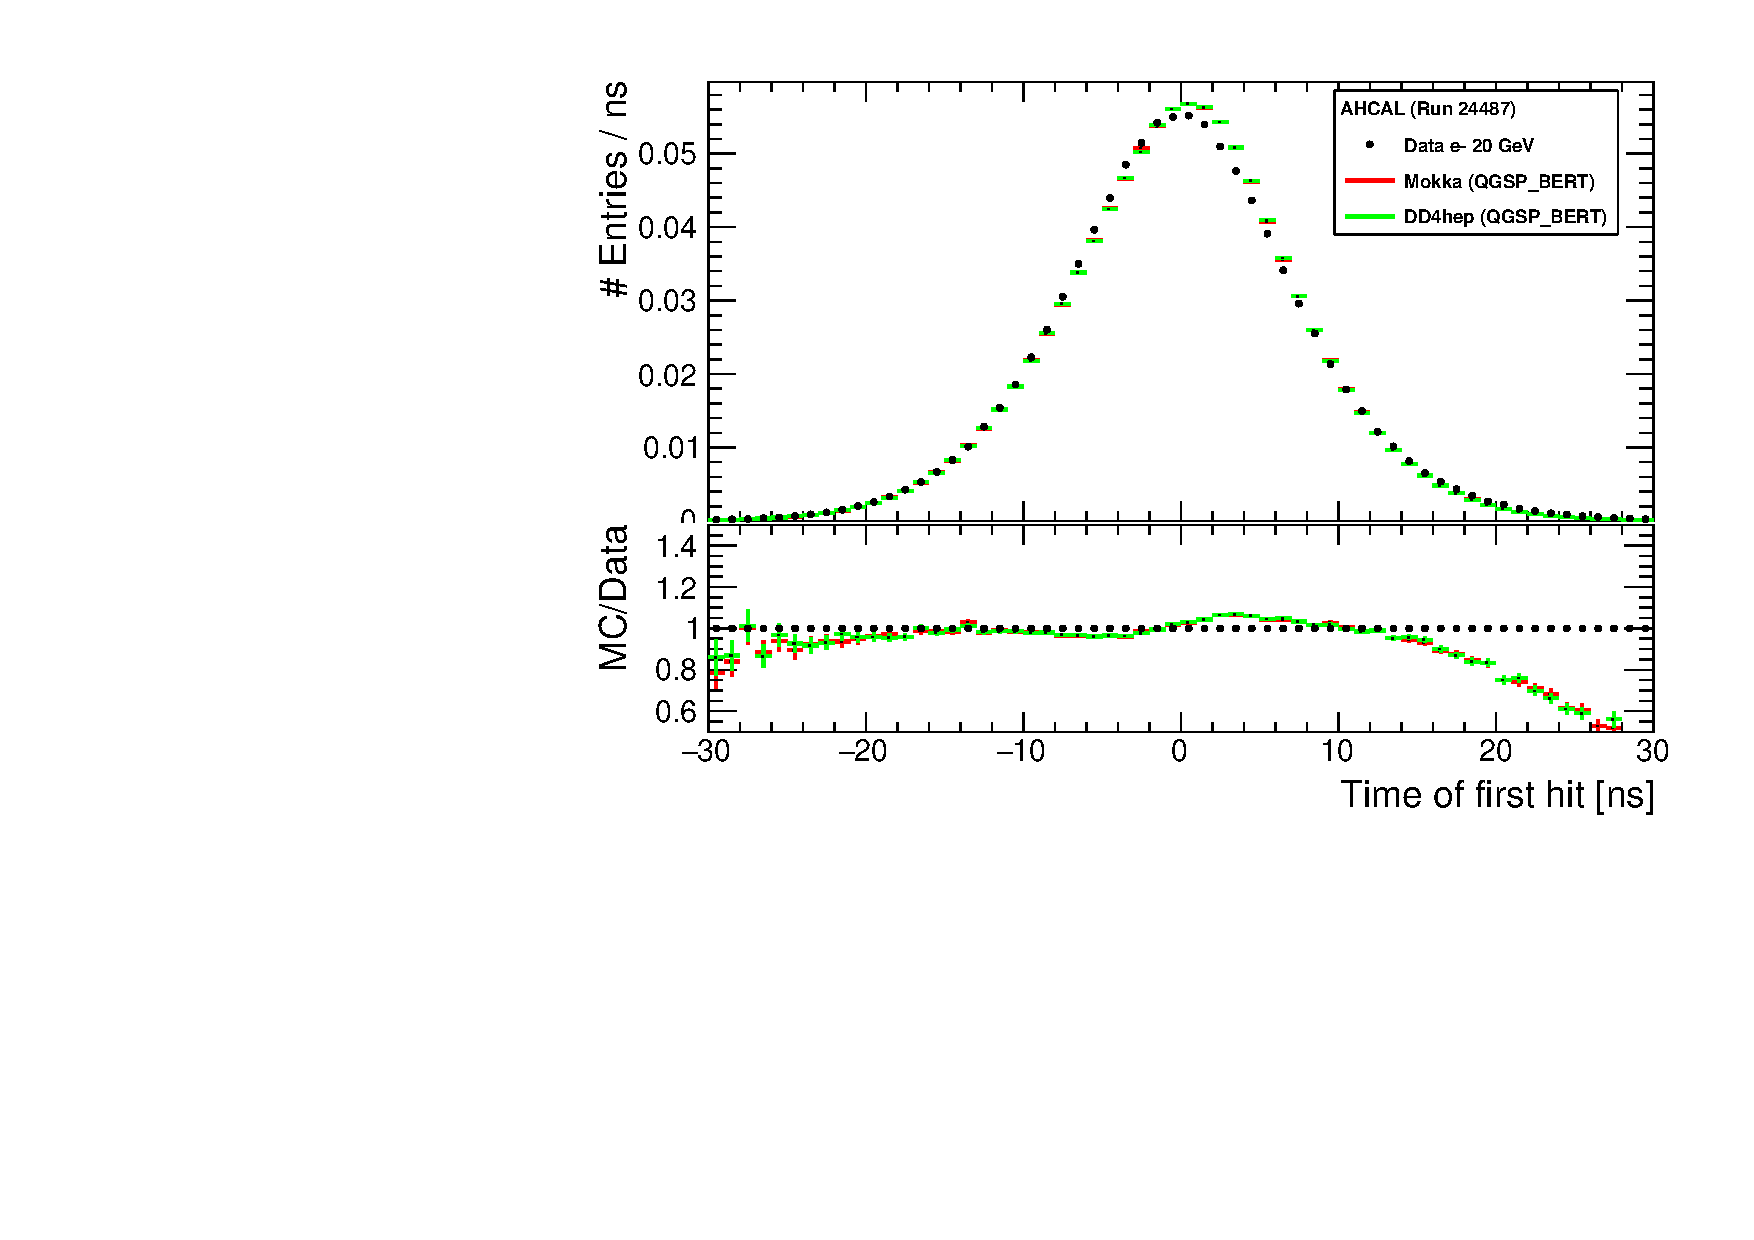
\includegraphics[width=0.5\textwidth]{fig/Simulation_Electrons/Comparison_SimData_Electrons_AfterCorrection.pdf}}\hfill
	\subfigure[Time of first hit for data and simulation zoomed between 1 and 200 ns.\label{fig:elec_sim_data_2}] {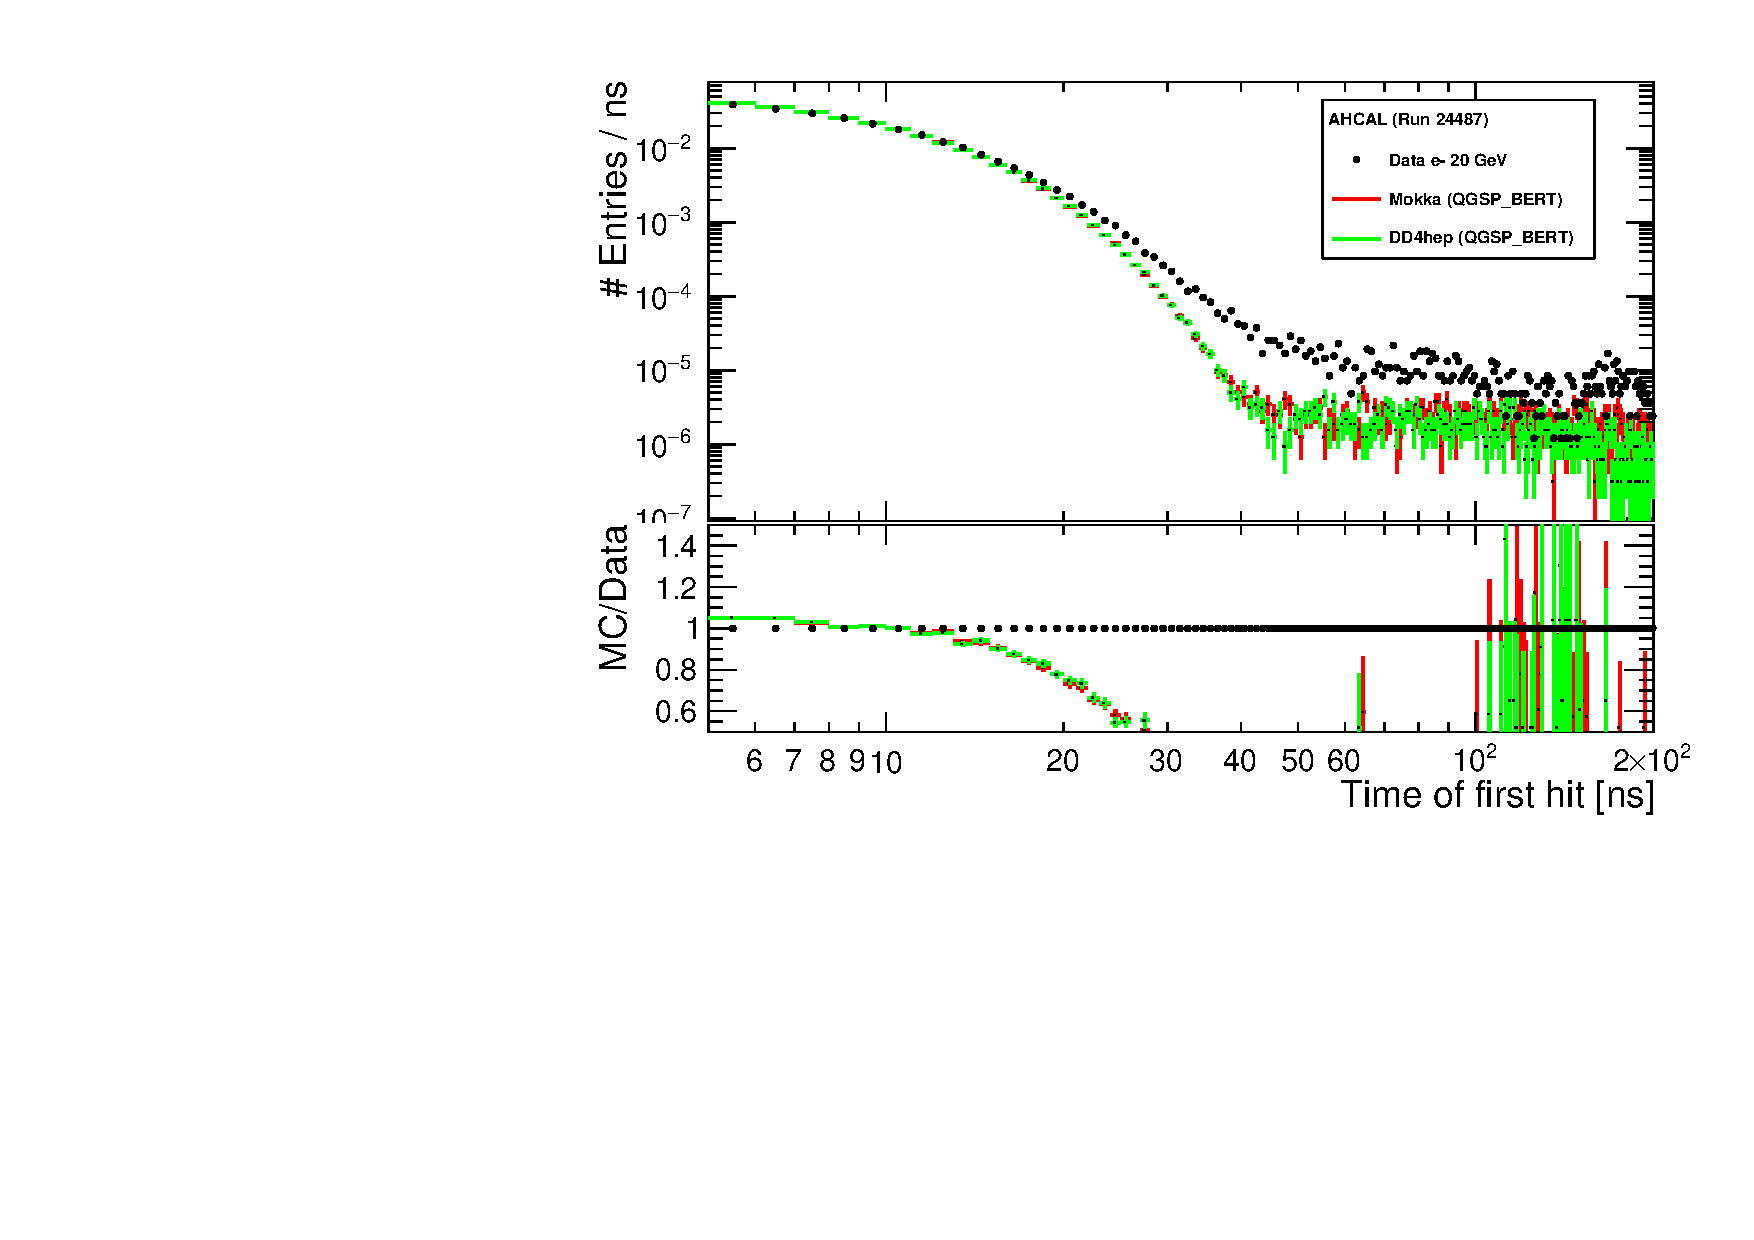
\includegraphics[width=0.5\textwidth]{fig/Simulation_Electrons/Comparison_SimData_Electrons_AfterCorrection_zoom.pdf}}
	\caption[]{\textbf{a}: The simulation in red does not fit to the data due to the dependence of the smearing with the number of hits above 0.5 MIPs. \textbf{b}: The simulation seems to fit the data in the first 10 ns up to 10\% then deviate fast that might be due to no noise implementation in the MC.}
	\label{fig:sim_data_elec}
\end{figure}
As shown on both figures, the simulation in red curve does not match the data. This is because of the number of hits effect that is present in data and that is highly dependent of the number of hits above 0.5 MIPs thus the number of noise hits (above 0.5 MIPs) could have an effect. So far the simulation and data does not match in terms of number of hits per events as shown on figure \ref{fig:nHitsEvent}. This might be due to noise hits above 0.5 MIPs that may be present more than expected and is not implemented in simulation.
\begin{figure}[htbp]
\begin{center}
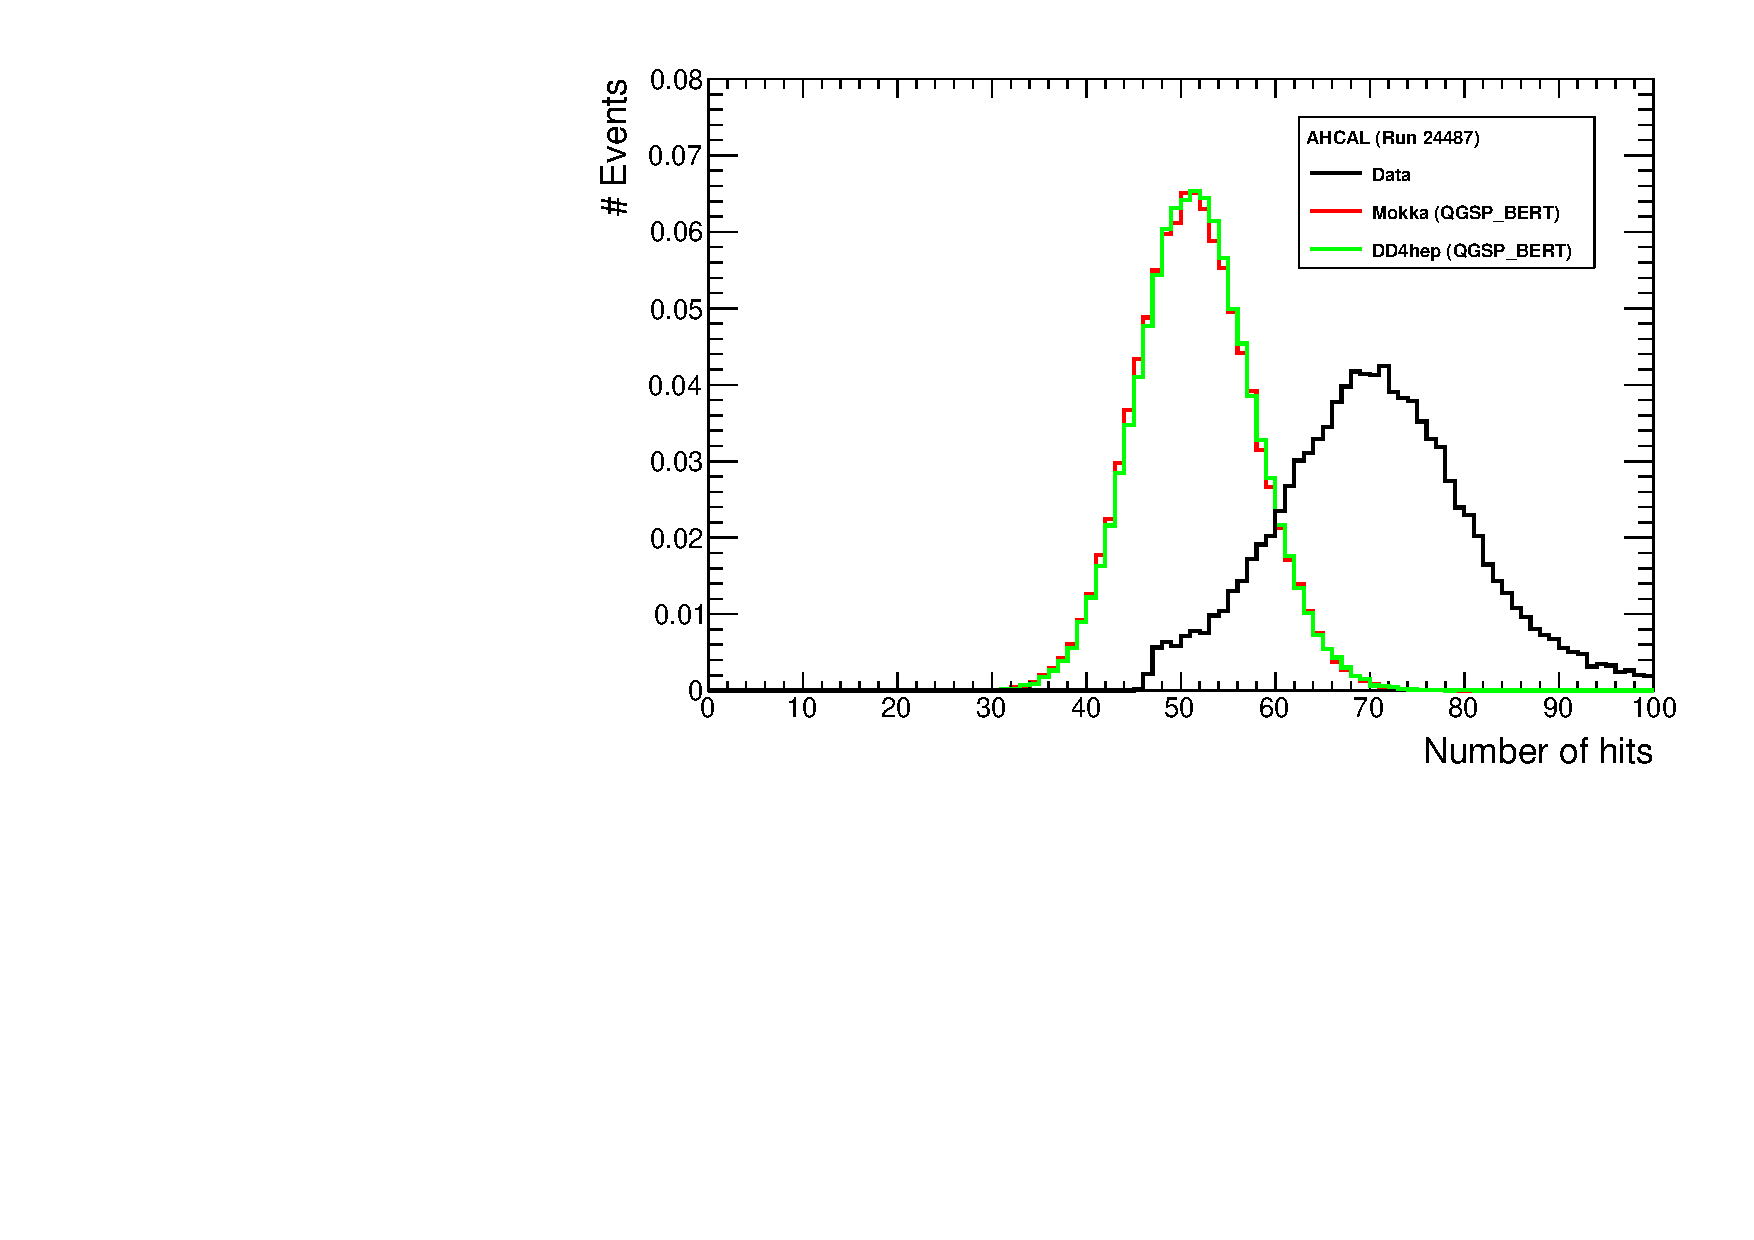
\includegraphics[width=0.6\textwidth]{fig/Electrons_BeamProfile/Run24487_nHits_AHCAL_20GeV_Comparison.pdf}
\caption{Comparison of the number of hits in data and MC for Run 24487. $\mu_{data}$ $\sim$ 70 and $\mu_{MC}$ $\sim$ 50. The difference is $\sim$ 20 hits which would account for less than 1\% of the channels.}
\label{fig:nHitsEvent}
\end{center}
\end{figure}
The right tail present in simulation is caused by small energy depositions from the electromagnetic shower corresponding to a very small fraction of events occurring ($\sim$0.1\%).

\section{Runs \& Event Selection}
 
During the SPS testbeam in July 2015, $\mu^-$, $e^-$ and $\pi^-$ runs were taken with beam momenta ranging from 10 GeV to 150 GeV. 
The runs and number of events used in this analysis are listed in table \ref{}.

\subsection{Pion Selection}

To be done!

\section{Results}

To be done!

\section{Summary}

\clearpage

\addcontentsline{toc}{section}{Bibliography}
\begin{thebibliography}{10}
\bibitem{ILC_TDR}
T.Behnke and al., \textit{The International Linear Collider Technical Design Report - Volume 4: Detectors}, \\
arXiv:1306.6329v1
\bibitem{IEEE_timing}
	A. Benaglia and al., \textit{Space-Time Development of Electromagnetic and Hadronic Showers and Perspectives for Novel Calorimetric Techniques}, \\
	IEEE TNS Vol.63-2, doi:10.1109/TNS.2016.2527758
\bibitem{SPSBeamLine}
	CERN, \textit{Secondary Beam \& Areas}, \\
	\href{http://sba.web.cern.ch/sba/BeamsAndAreas/h2/H2manual.html}{http://sba.web.cern.ch/sba/BeamsAndAreas/h2/H2manual.html}
\bibitem{CAN-038}
	The CALICE Collaboration, \textit{The Time Structure of Hadronic Showers in Tungsten and Steel with T3B}, \\
	CALICE Analysis Note CAN-038
\bibitem{AHCAL_Physics}
	The CALICE Collaboration, \textit{Validation of GEANT4 Monte Carlo models with a highly granular scintillator-steel hadron calorimeter}, \\
	2013 JINST 8 P07005, doi:10.1088/1748-0221/8/07/P07005
\bibitem{SPIROCManual}
	Omega Group, \textit{SPIROC Manuel}, \\
	\href{http://omega.in2p3.fr/index.php/download-center/doc_view/165-spiroc2-datasheet.raw?tmpl=component}{http://omega.in2p3.fr/index.php/download-center/doc\_view/165-spiroc2-datasheet.raw?tmpl=component}
\bibitem{OskarSSP}
	 O. Hartbrich, \textit{Investigation of the time measurement capabilities of the SPIROC2b ASIC}, \\
	 DESY summer student report, 2011.
\bibitem{EldwanSSP}
	 E. Brianne, \textit{Studies of the front-end electronics of the Analog HCAL}, \\
	 DESY summer student report, 2012.
\bibitem{OskarMaster}
	 O. Hartbrich, \textit{Commissioning and LED System Tests of the Engineering Prototype of the Analog Hadronic Calorimeter of the CALICE Collaboration}, \\
	 DESY-thesis-2012-040, ISSN 1435-8085.
\bibitem{CAN-002} 
	 The CALICE Collaboration, \textit{First results from electron data with the CALICE tile HCAL prototype at the CERN test-beam}, \\
	 CALICE Analysis Note CAN-002
\bibitem{CAN-010} 
	 The CALICE Collaboration, \textit{Electron data with the CALICE tile AHCAL prototype at the CERN test-beam - Update}, \\
	 CALICE Analysis Note CAN-010
\bibitem{JINST-6}
	 The CALICE Collaboration, C. Adloff et al., \textit{Electromagnetic response of a highly granular hadronic calorimeter}, \\
	 2011 JINST 6 P04003, doi:10.1088/1748-0221/6/04/P04003
\bibitem{DAQ}
	 T. Suehara and al., \textit{AIDA-CALICE DAQ interface} \\
	 AIDA 2020 Scientific/Technical Note, AIDA-2020-NOTE-2016-006
\end{thebibliography}

\clearpage
\begin{appendix}
\section*{Appendix}
\pagestyle{plain}
%\setcounter{table}{0}
\renewcommand{\thetable}{A\arabic{table}}
\addcontentsline{toc}{section}{Appendix}
\addtocontents{toc}{\protect\setcounter{tocdepth}{0}}

\section{Error Estimation of the TDC calibration.}
\label{appendix:calib_error}

In this appendix, a small study of the error made on the calibration from TDC to nanoseconds is done. By simple calculation, the conversion is done is the following way:
\begin{equation*}
\begin{split}
\text{T} \: \text{[ns]} & = ( \text{TDC} - \text{Ped} ) * \text{slope} \\
& = ( \text{TDC} - \text{Ped} ) * \frac{\text{A}}{(\text{Max} - \text{Ped})} \quad \text{with A = 3920 ns}
\end{split}
\end{equation*}
To avoid correlations between the slope and the pedestal, the error is obtained by differentiating w.r.t Max and Ped. The error is then obtained via:
\begin{equation*}
\partial t^2 = \left(\frac{\partial t}{\partial Ped}\right)^2 \times \sigma_{Ped}^2 + \left(\frac{\partial t}{\partial Max}\right)^2 \times \sigma_{Max}^2 + \left(\frac{\partial t}{\partial A}\right)^2 \times \sigma_{A}^2
\end{equation*}
Assuming that $\sigma_{A}$ is null, we get the following formula:
\begin{equation*}
\partial t^2 = \frac{1}{(\text{Max} - \text{Ped})^2} \left[ \left( \frac{\text{A(TDC - Max)}}{(\text{Max} - \text{Ped})} \right)^2 \times \sigma_{Ped}^2 + \left( \frac{\text{A(TDC - Ped)}}{(\text{Max} - \text{Ped})} \right)^2 \times \sigma_{Max}^2 \right]
\end{equation*}
As one can expect, the formula is symmetric and should be minimum in the middle of the ramp as long as $\sigma_{Max}$ and $\sigma_{Ped}$ are similar. On the other hand, the error will be greater on one side or the other depending on the $\sigma$ being the biggest. 
\begin{figure}[htbp]
	\subfigure[Errors extracted from the edge detection for the pedestal for each chip. channel, memory-cell and BXID.\label{fig:error_ped}] {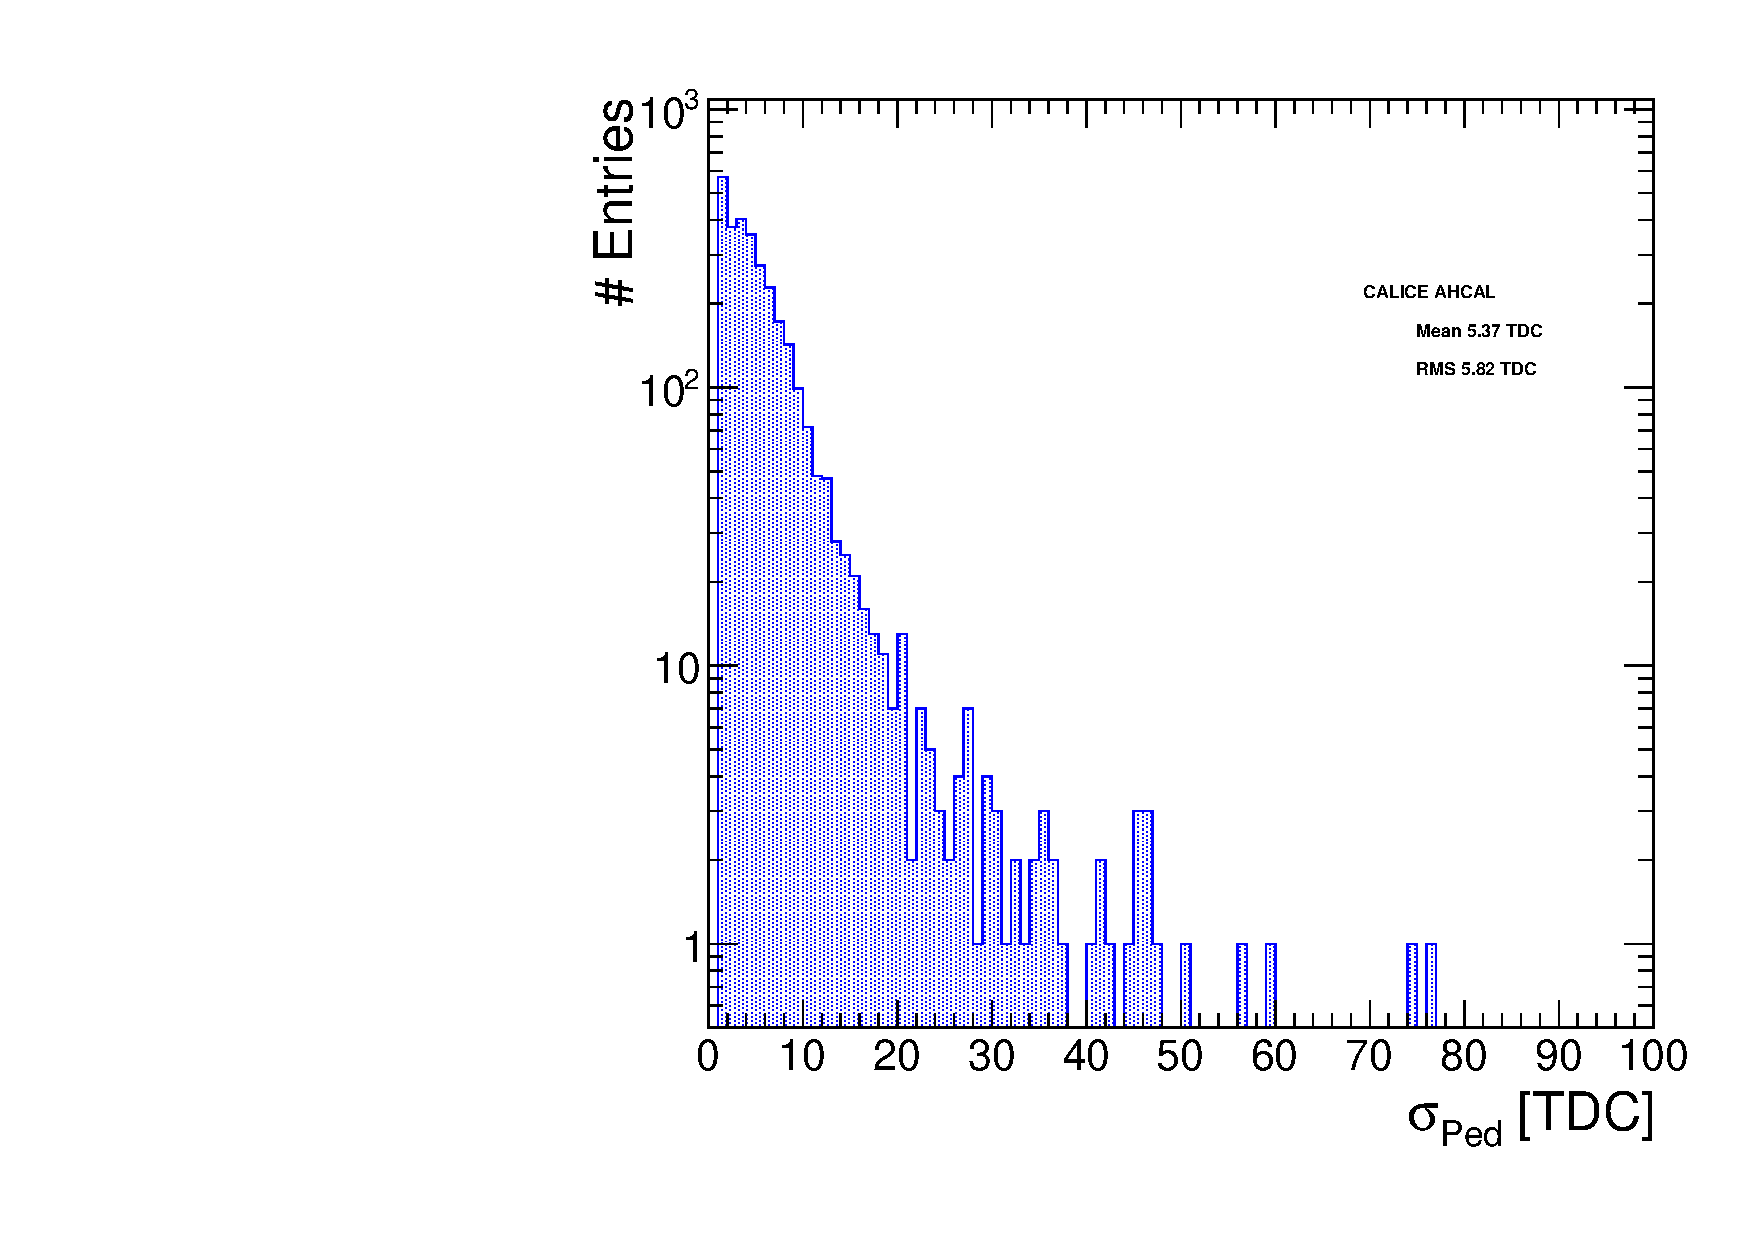
\includegraphics[width=0.5\textwidth]{fig/PedestalErrorDistribution_AHCAL.pdf}}\hfill
	\subfigure[Error extracted from the edge detection for the maximum of the ramp for each chip and BXID.\label{fig:error_max}] {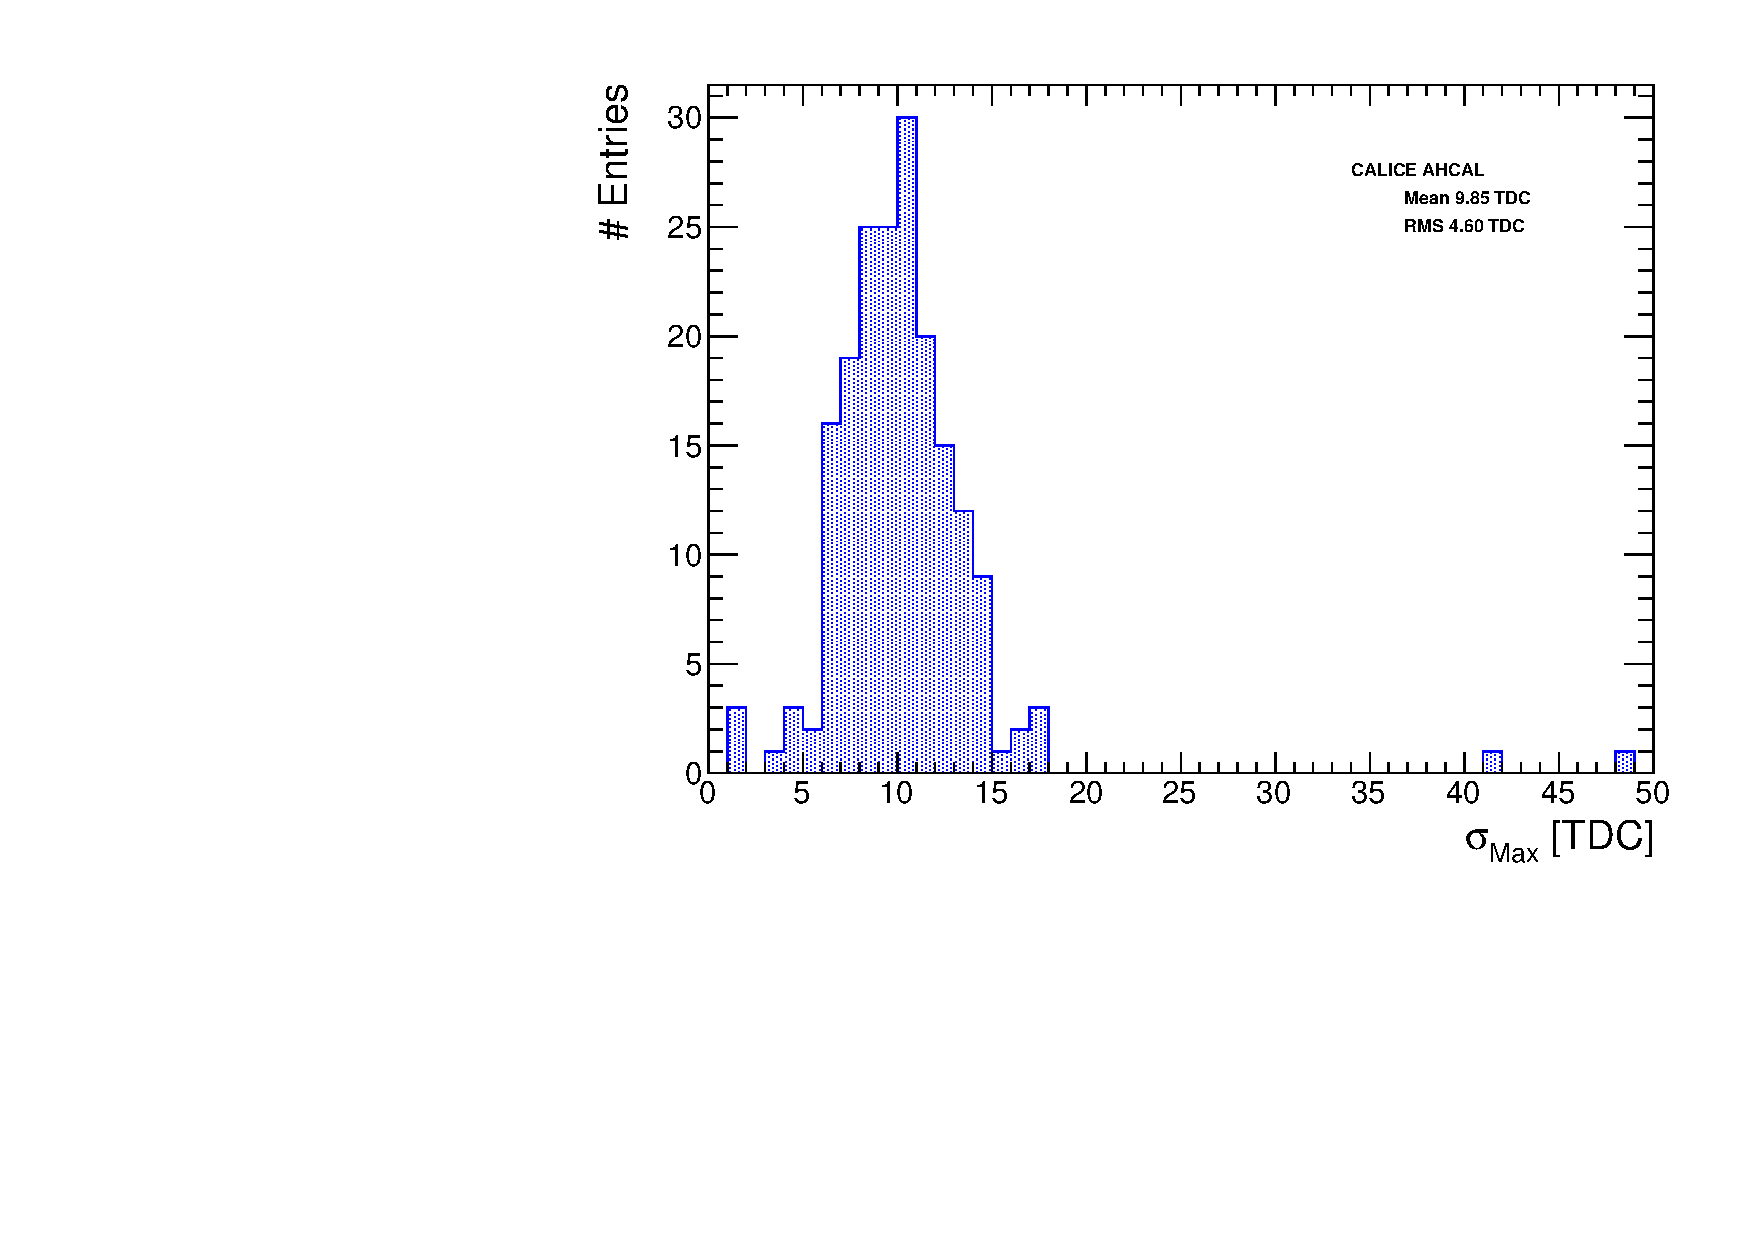
\includegraphics[width=0.5\textwidth]{fig/MaxErrorDistribution_AHCAL.pdf}}
	\caption[]{\textbf{a}: Pedestal error distribution extracted for all channels in the detector, most of the errors made are small with a high tail certainly due to the limited statistics for some channels. $\mu$ = 5.37 TDC, RMS = 5.82 TDC \textbf{b}: Maximum error distribution extracted from the edge detection method for each chip and BXID. The error is a bit higher than for the pedestal in general due to the difficulty to detect perfectly the end of the ramp. $\mu$ = 9.85 TDC, RMS = 4.60 TDC.}
	\label{fig:error_dist}
\end{figure}
The errors estimations $\sigma_{Max}$ and $\sigma_{Ped}$ are described in subsection \ref{subsec:slope_calib}. Distributions of the errors extracted can be seen on figures \ref{fig:error_ped} and \ref{fig:error_max}. Theses errors are obtained arbitrary due to the threshold and maximum variation and are likely to be over-estimated as they are not reflected in the final timing distribution. Moreover, the shift of the distribution to zero is correcting any error made on the pedestal for each channels thus $\sigma_{Ped}$ is likely very small. 
\begin{figure}[htbp]
	\subfigure[Calibration error made on the conversion to nanosecond for a channel on layer 3.\label{fig:error_chn}] {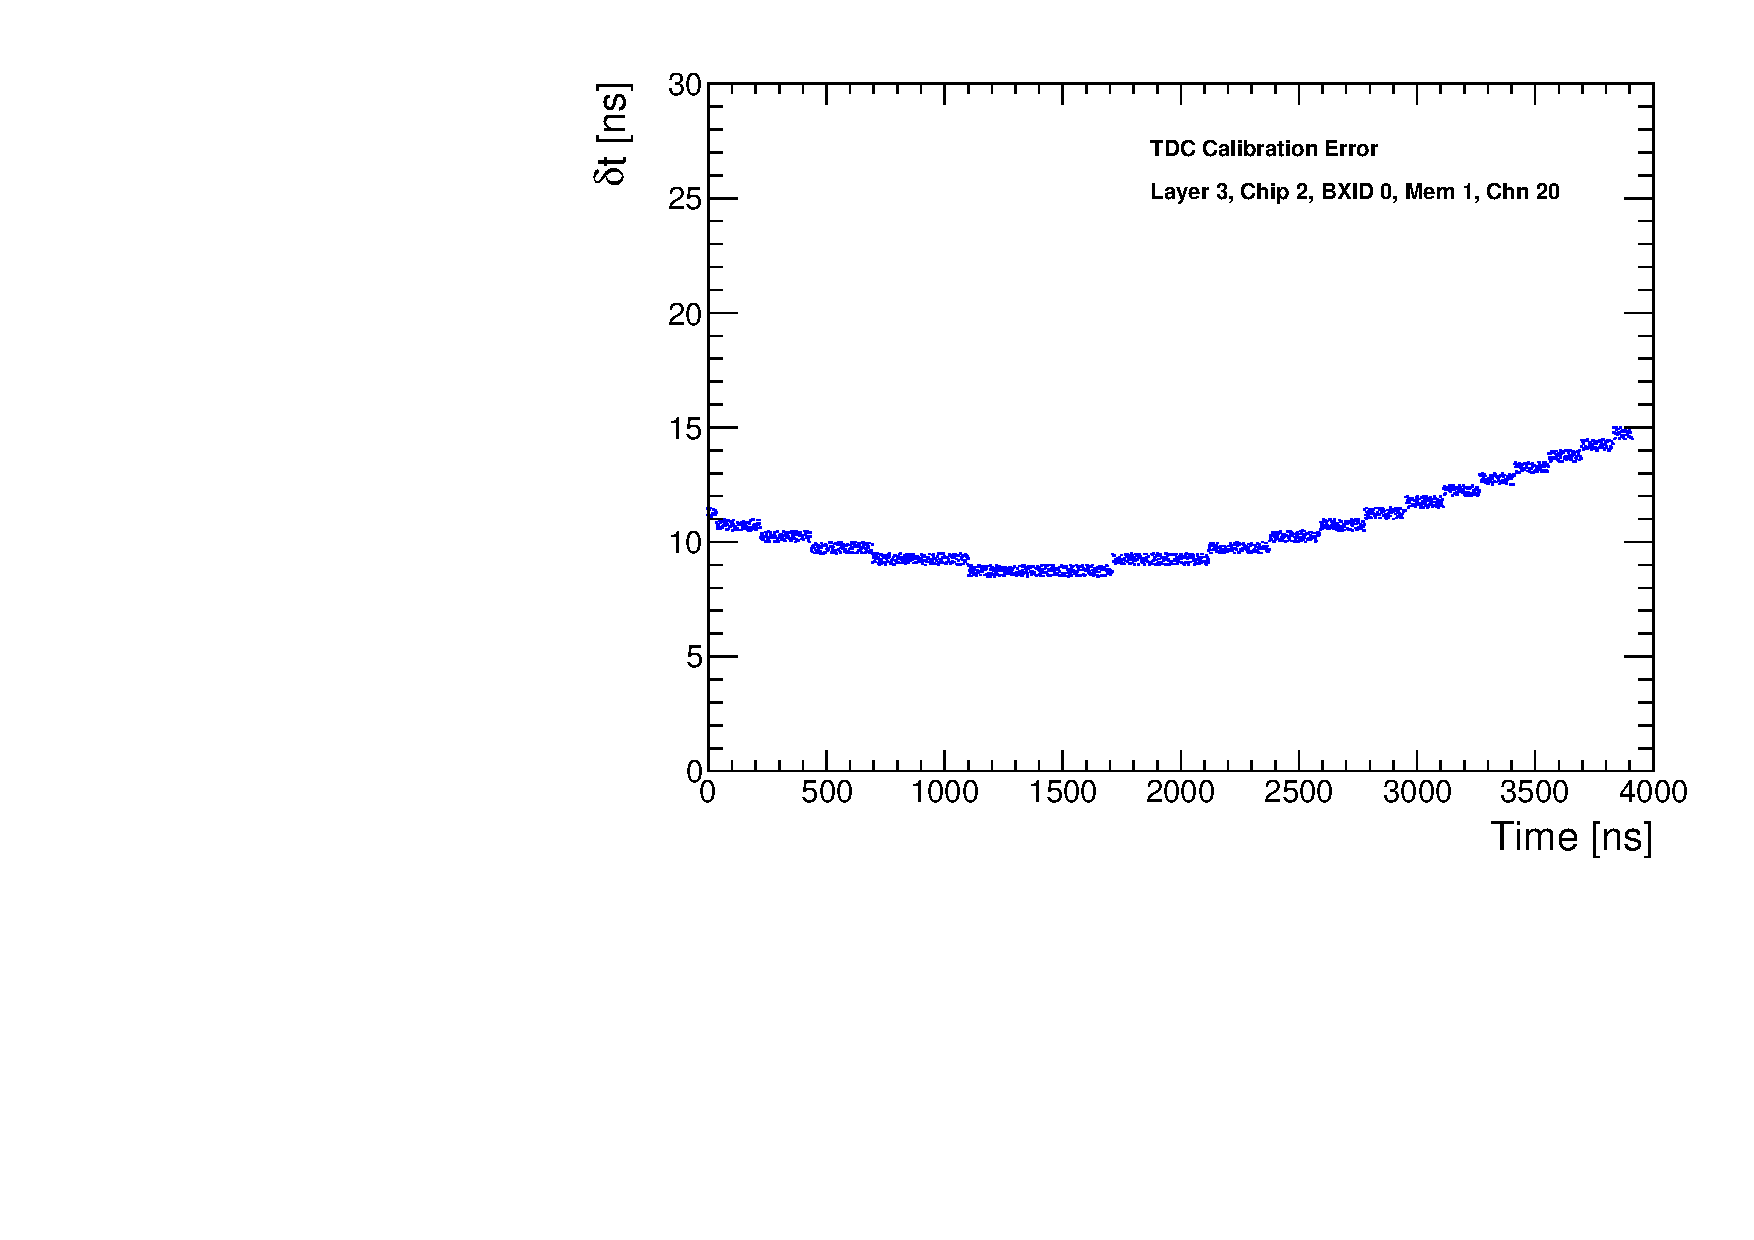
\includegraphics[width=0.5\textwidth]{fig/TimeErrorEstimation_Layer3.pdf}}\hfill
	\subfigure[Calibration error made on the conversion to nanosecond for a channel on layer 5.\label{fig:error_chn2}] {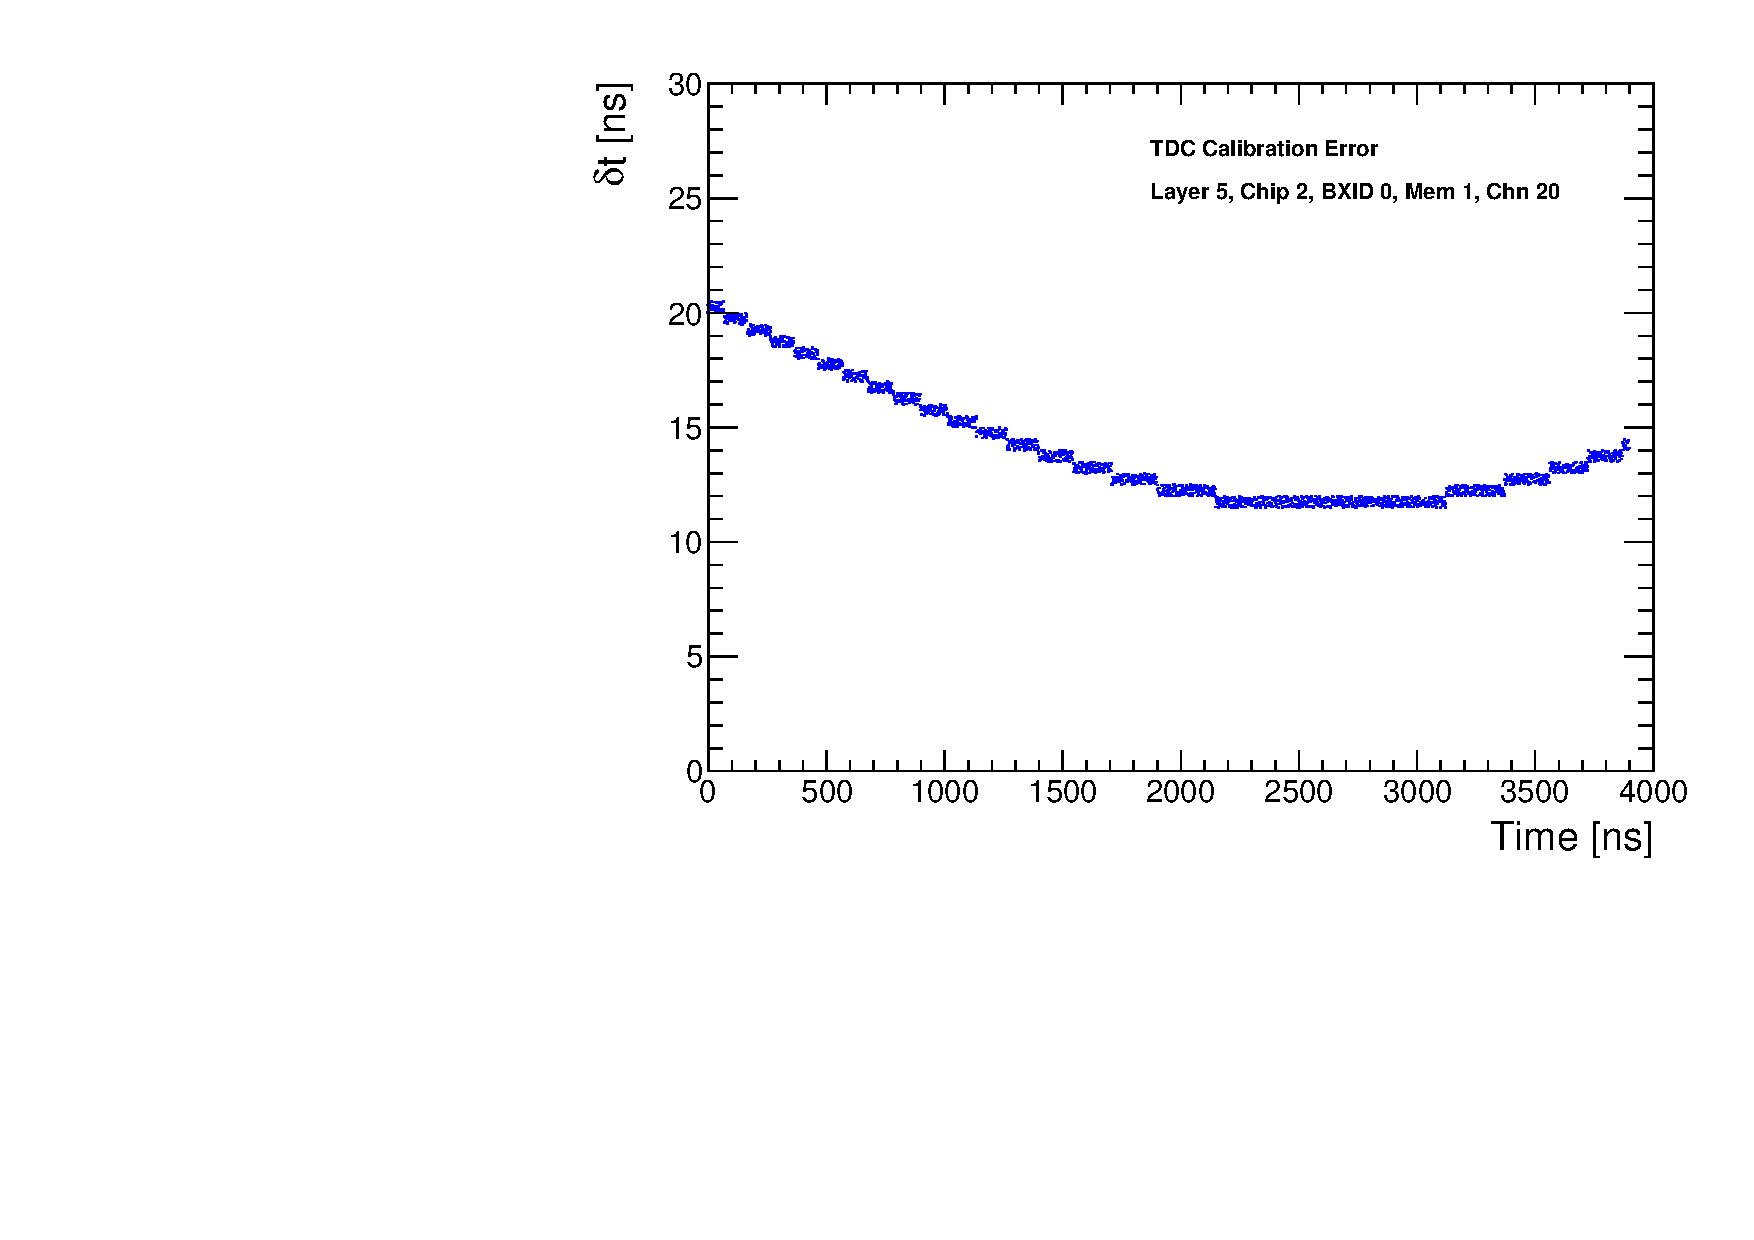
\includegraphics[width=0.5\textwidth]{fig/TimeErrorEstimation_Layer5.pdf}}
	\caption[]{\textbf{a}: Error distribution made for a single channel on layer 3. The error is variating between 9 and 14 ns but is likely to be over-estimated and not valid for the final time distribution. \textbf{b}: Error distribution made for a single channel on layer 5. The error is variating between 12 and 20 ns but is likely to be over-estimated and not valid for the final time distribution.}
	\label{fig:error_calibration}
\end{figure}
The figure \ref{fig:error_chn2} represent the error made for one channel selected in a single chip for a single memory cell and BXID. It shows the symmetric behaviour of the error and present a minimum around the middle of the ramp. This not a typical channel as mostly the maximum has an error higher than the pedestal due to the difficulty to pick perfectly the maximum of the ramp with the sharp falling edge. A more typical channel can be seen on figure \ref{fig:error_chn}.

\newpage
\section{Influence of the number of triggered channels and parametrisation in Monte-Carlo.}
\label{appendix:ped_shift}

The correction applied function of the number of hits above 0.5 MIPs is only a global correction not an event to event basis correction. Thus a part of the effect remains in the time distribution or it may be another effect from the electronics that is not yet identified.\\
This effect has to be implemented in the simulation in order to match the timing distribution of electrons without also influencing the time distribution for muons. A parametrisation is thus implemented in the Monte-Carlo extracted from data. This parametrisation assumes the following, the effect is additional to the seen muon resolution giving then:
\begin{equation*}
\begin{split}
& \text{RMS}_{\text{obs}}^2 = \text{RMS}_{\mu}^2 + \text{RMS}_{\text{effect}}^2 \\
& \Leftrightarrow \text{RMS}_{\text{effect}} = \sqrt{\text{RMS}_{\text{obs}}^2 - \text{RMS}_{\mu}^2}
\end{split}
\end{equation*}
The $\text{RMS}_{\text{PedShift}}$ is then extracted from data by fitting with a Gaussian the timing distribution obtained for each bin in number of triggered channels in a chip as shown in figure \ref{fig:ped_shift_dist_para}. By plotting the Gaussian width extracted function of the number of triggered channels in a chip, one can extract the parametrisation of the effect. The $\text{RMS}_{\mu}$ is assumed to be 4.95 ns as shown in figure \ref{fig:timing_electron_muon_comp}. The figure \ref{fig:para_fit} is fitted with a function in the shape:
\begin{equation*}
\text{RMS}_{\text{effect}} = A \times Log( \epsilon * x )
\end{equation*}
\begin{figure}[htbp]
	\subfigure[Time of the first hit distribution for different binning of number of triggered channels in a chip.\label{fig:ped_shift_dist_para}] {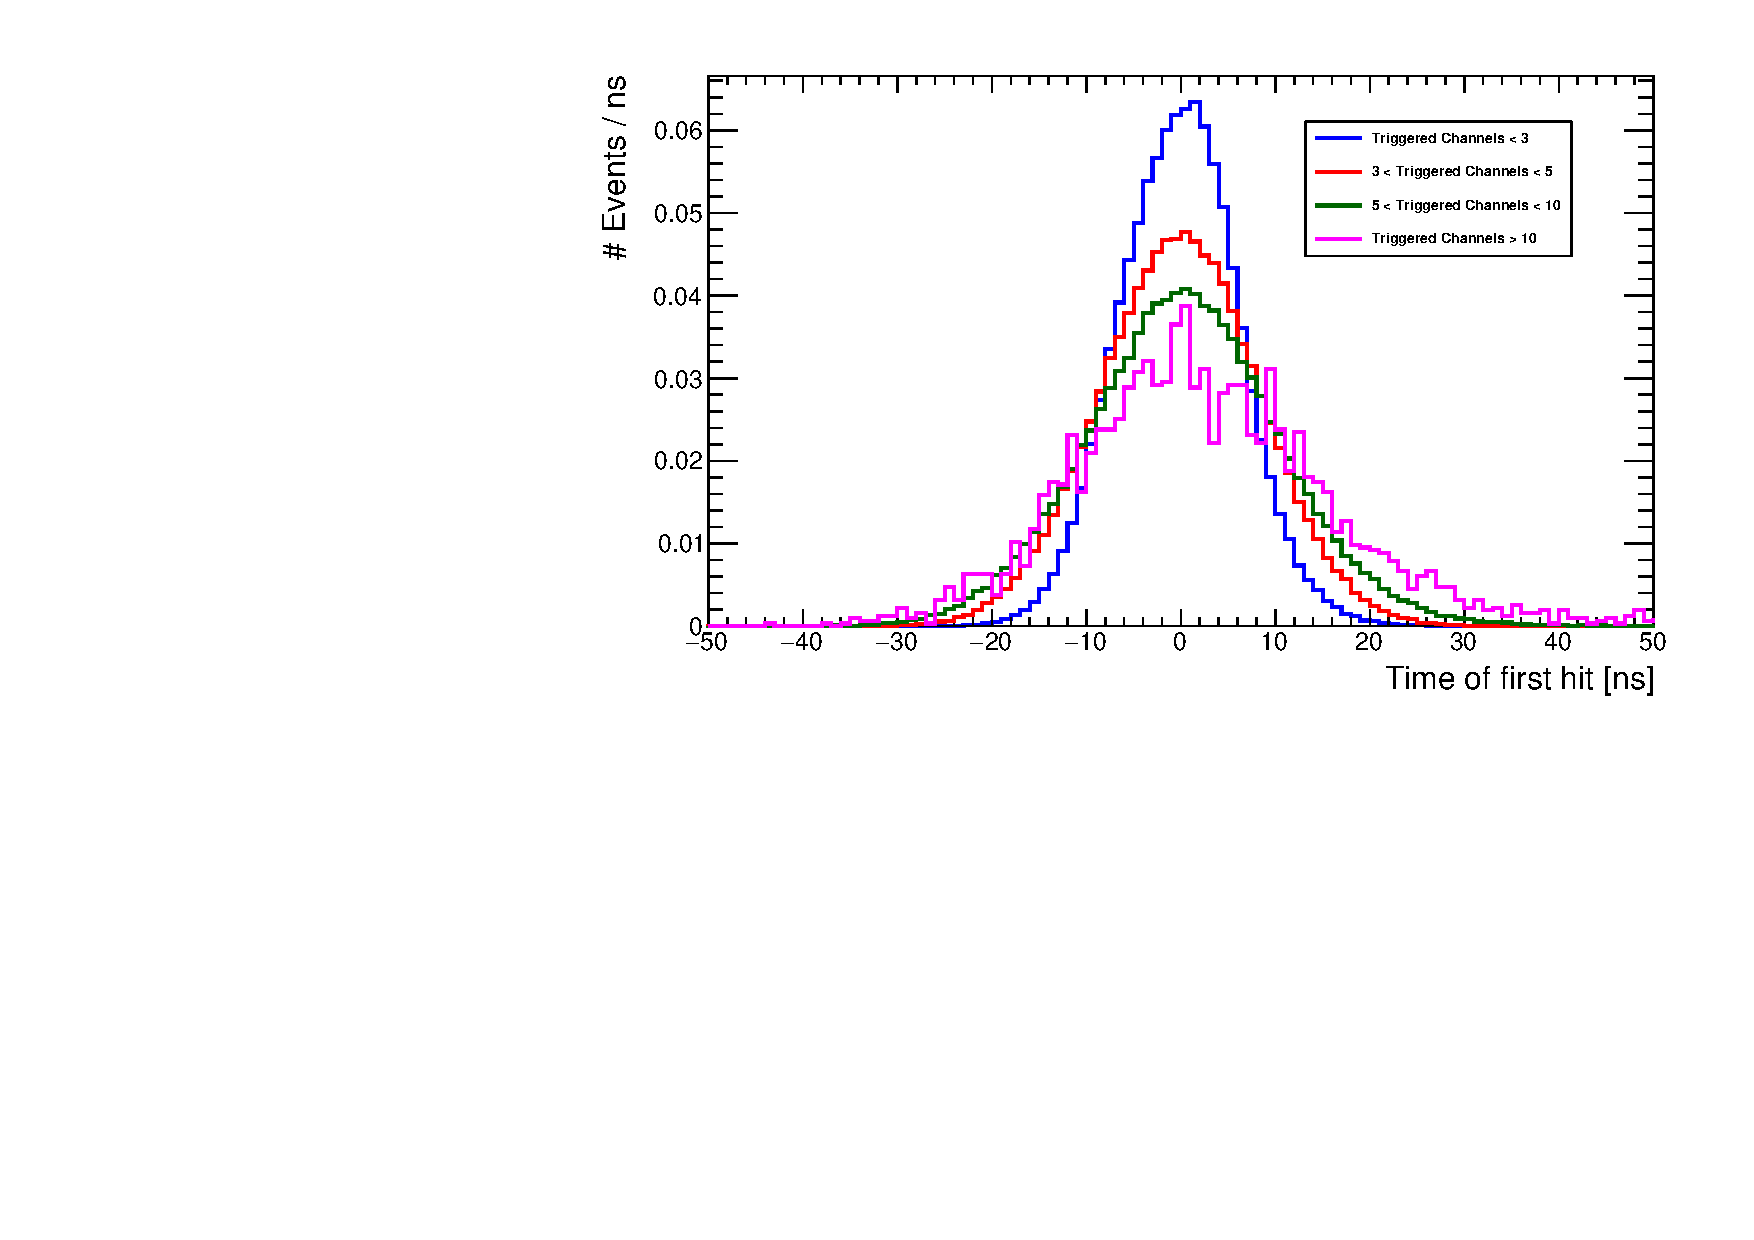
\includegraphics[width=0.5\textwidth]{fig/TimingHitsBins.pdf}}\hfill
	\subfigure[Gaussian width extracted function of the number of triggered channels in a chip.\label{fig:para_fit}] {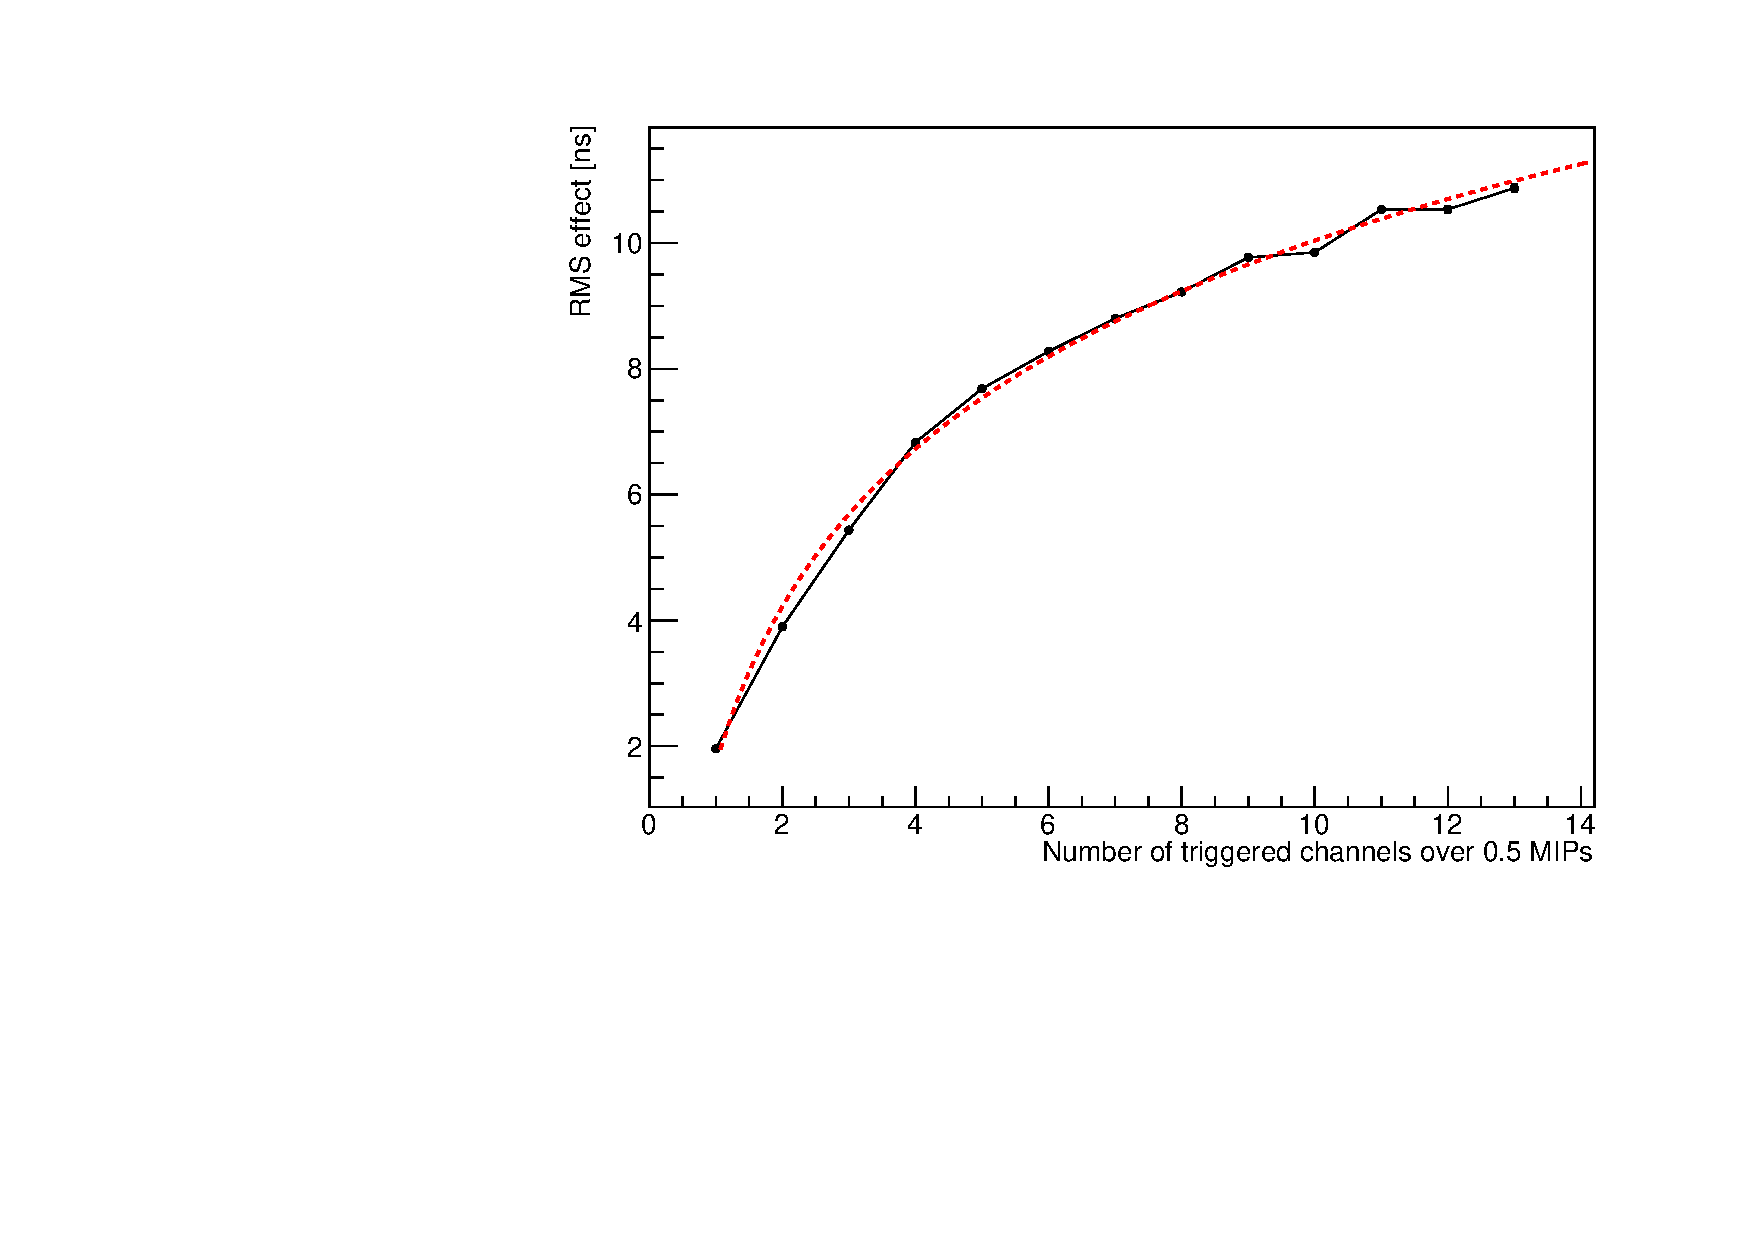
\includegraphics[width=0.5\textwidth]{fig/ParametrisationPedestalShift_only.pdf}}
	\caption[]{\textbf{a}: The Gaussian width is increasing with the number of triggered channels in a chip due to the remaining of the pedestal shift effect. The mean of the distribution shift slightly with increasing number of triggers but is neglected. \textbf{b}: Extracted width for each bins of number of triggered channels in a chip. The parameters are : A = 8.32 $\pm$ 0.03, $\epsilon$ = 1.61 $\pm$ 0.01 and $\chi^2$ = 37.}
	\label{fig:mc_para}
\end{figure}

\newpage
\section{Study of noise on timing.}
\label{appendix:noise_timing}


\end{appendix}
\end{document}
